\documentclass[sigconf]{acmart}
%\documentclass{style/sig-alternate}

\usepackage{lmodern}
\usepackage[utf8]{inputenc}
\usepackage[TS1,T1]{fontenc}
\usepackage[usenames,dvipsnames,svgnames,table]{xcolor}
\usepackage{url}
\usepackage{graphicx}
\DeclareGraphicsExtensions{.eps}
\usepackage{latexsym}
\usepackage{xspace}
\usepackage{enumitem}
\usepackage{subcaption}
\usepackage{flushend}
\usepackage{algorithm}
\usepackage{algorithmic}
\usepackage{amsmath}
\usepackage{bm}
\usepackage{listings}
\usepackage{cleveref}

\setenumerate{noitemsep,topsep=0pt,parsep=0pt,partopsep=0pt}


% Enviroment definitions
\newtheorem{definition}{Definition}[section]
\newtheorem{proposition}{Proposition}
\newtheorem{conjecture}{Conjecture}
\newtheorem{theorem}{Theorem}
\newtheorem{problem}{Problem}
\newtheorem{example}{Example}
\newtheorem{remark}{Remark}

% Comments
\newcommand{\todo}[1]{[\textcolor{magenta}{{\bf TODO: }#1}]}
\newcommand{\reminder}[1]{[\textcolor{magenta}{{\bf NB: }#1}]}
\newcommand{\comment}[1]{\noindent\textcolor{comcol}{\small\textbf{Comment:} #1}}
\newcommand*{\eat}[1]{}
\newcommand{\julia}[1]{[\textcolor{purple}{{\bf Julia: }#1}]}
\newcommand{\vera}[1]{[\textcolor{orange}{{\bf Vera: }#1}]}

% Vocabulary
\newcommand*{\ql}{\textsf{Portal}\xspace}
\newcommand*{\tg}{\textsf{TGraph}\xspace}
\newcommand*{\tgs}{\textsf{TGraphs}\xspace}
\newcommand*{\rgs}{\textsf{representative graphs}\xspace}
\newcommand*{\ve}{\textsf{vertex-edge}\xspace}
\newcommand*{\sg}{RG\xspace}
\newcommand*{\rg}{RG\xspace}
\newcommand*{\mg}{MG\xspace}
\newcommand*{\mgc}{MGC\xspace}
\newcommand*{\og}{OG\xspace}
\newcommand*{\ogc}{OGC\xspace}
\newcommand*{\hg}{HG\xspace}

\newcommand*{\trg}{\ensuremath{\mathsf{T^{RG}}}\xspace}
\newcommand*{\tve}{\ensuremath{\mathsf{T^{VE}}}\xspace}
%\newcommand*{\tgg}{\textsf{TG}\xspace}
\newcommand*{\tgg}{\ensuremath{\mathsf{T^{RG}}}\xspace}
\newcommand*{\tv}{\textsf{TV}\xspace}
\newcommand*{\te}{\textsf{TE}\xspace}
\newcommand*{\avv}{\ensuremath{\mathsf{A^{V}}}}
\newcommand*{\aee}{\ensuremath{\mathsf{A^{E}}}}
\newcommand*{\tav}{\ensuremath{\mathsf{TA^{V}}}}
\newcommand*{\tae}{\ensuremath{\mathsf{TA^{E}}}}

\newcommand*{\opp}{\textsf{op}\xspace}
\newcommand*{\cl}{\textsf{coalesce}\xspace}
\newcommand{\dollar}{{\$}}

% Time periods
\newcommand{\tpy}[1]{#1}
\newcommand{\tpym}[2]{#1/#2}
\newcommand{\tpymd}[3]{\ensuremath{\mathsf #1/#2/#3}}

% Query langauge operations
\newcommand*{\tsel}[2]{\ensuremath{\sigma^{t}(#1,#2)}}
\newcommand*{\ssel}[2]{\ensuremath{\sigma^{s}(#1,#2)}}

\newcommand*{\andgrp}[4]{\ensuremath{\gamma^{\cap}(#1,#2,#3,#4)}}
\newcommand*{\orgrp}[4]{\ensuremath{\gamma^{\cup}(#1,#2,#3,#4)}}

\newcommand*{\xfrm}[3]{\ensuremath{\chi(#1,#2,#3)}}
\newcommand*{\an}[2]{\ensuremath{\alpha(#1,#2)}}

%\newcommand*{\tor}[4]{\ensuremath{\bigcup({#1},{#2},{#3},{#4})}}
\newcommand*{\tor}[4]{\ensuremath{#1 \cup_{#3, #4} #2}}
%\newcommand*{\tand}[4]{\ensuremath{\bigcap(#1,#2,#3,#4)}}
\newcommand*{\tand}[4]{\ensuremath{#1 \cap_{#3, #4} #2}}

\newcommand{\insql}[1]{\textsf{#1}}

\newcommand*{\predName}[1]{\ensuremath{\mathsf{#1}}}
\newcommand*{\pred}[3]{#1~\predName{#2}~#3}

\newcommand*{\op}[1]{\ensuremath{\mathsf{#1}}}
\def\ojoin{\setbox0=\hbox{$\Join$}%
\rule[0.2ex]{.25em}{.4pt}\llap{\rule[1.5ex]{.25em}{.4pt}}}
\def\leftouterjoin{\mathbin{\ojoin\mkern-5.8mu\Join}}
\def\rightouterjoin{\mathbin{\Join\mkern-5.8mu\ojoin}}
\def\fullouterjoin{\mathbin{\ojoin\mkern-5.8mu\Join\mkern-6mu\ojoin}} 

%\lstset{frame=tb,
%  language=scala,
%  aboveskip=3mm,
%  belowskip=3mm,
%  showstringspaces=false,
%  columns=flexible,
%  basicstyle={\small\ttfamily},
%  numbers=none,
%  numberstyle=\tiny\color{gray},
%  keywordstyle=\color{blue},
%  commentstyle=\color{dkgreen},
%  stringstyle=\color{mauve},
%  breaklines=true,
%  breakatwhitespace=true,
%  tabsize=3
%}
%\lstset{language=scala}



\clubpenalty=10000 
\widowpenalty = 10000
\tolerance=10000

\begin{document}

\title{Temporal Graph Algebra}
%\title{Querying Evolving Graphs with SystemXYZ}

%\numberofauthors{2}
%\author{
%  \alignauthor Vera Zaychik Moffitt\\
%  \affaddr{Drexel University}\\
%  \email{zaychik@drexel.edu}  \and
%
%  \alignauthor Julia Stoyanovich\\
%  \affaddr{Drexel University}\\
%  \email{stoyanovich@drexel.edu}  \\
 %
%}
\author{Vera Zaychik Moffitt}
\affiliation{%
  \institution{Drexel University, USA}
}
\email{zaychik@drexel.edu}

\author{Julia Stoyanovich}
\authornote{This work was supported in part by NSF Grants No. 1464327 and 1539856, and BSF Grant No. 2014391.}
\affiliation{%
  \institution{Drexel University, USA}
}
\email{stoyanovich@drexel.edu}

\begin{abstract}

Graphs are used to represent a plethora of phenomena, from the Web and
social networks, to biological pathways, to semantic knowledge
bases. Arguably the most interesting and important questions one can
ask about graphs have to do with their evolution. Which Web pages are
showing an increasing popularity trend? How does influence propagate
in social networks? How does knowledge evolve?  

In this paper we present our ongoing work on the \ql system, an
open-source distributed framework for evolving graphs.  \ql
streamlines exploratory analysis of evolving graphs, making it
efficient and usable, and providing critical tools to computational
and data scientists.  Our system implements a declarative query
language by the same name, which we briefly describe in this paper.
Our basic abstraction is a \tg, which logically represents a series of
adjacent snapshots.  We present different physical representations of
\tgs and show results of a preliminary experimental evaluation of
these physical representations for an important class of evolving
graph analytics.

\end{abstract}


\copyrightyear{2017} 
\acmYear{2017} 
\setcopyright{acmcopyright}
\acmConference{DBPL 2017}{September 1, 2017}{Munich, Germany}\acmPrice{15.00}\acmDOI{10.1145/3122831.3122838}
\acmISBN{978-1-4503-5354-0/17/09}

\ccsdesc[500]{Information systems~Graph-based database models}
\ccsdesc[500]{Information systems~Temporal data}
\ccsdesc[500]{Information systems~Query languages}

\keywords{Evolving Graphs; Temporal Databases}

\maketitle

\thispagestyle{empty}

\section{Introduction}
\label{sec:intro}

Evolving graphs analysis is a rich new area of research that has been
getting increasing
attention~\cite{DBLP:journals/csur/AggarwalS14,Miao2015,Ren2011,Semertzidis2015}.
This is a natural consequence of the prevalence of graph datasets to
represent such wide-ranging phenomena as social networks and the Web.
The phenomena change with time, and the evolution provides another
dimension of interest from which to draw insight.

Given the progress both in the area of graph databases and temporal
databases, it is expected that evolving graphs would be supported as
well, being at the intersection of the two areas.  And yet, systematic
support for scalable querying and analytics over evolving graphs still
lacks, despite much recent interest and activity and despite increased
variety and availability of evolving graph data.  This support is
urgently needed, due to the scalability and efficiency challenges
inherent in evolving graph analysis, and to considerations of
usability and ease of dissemination.  The goal of our work is to fill
this gap by combining the advances in graph databases and temporal
relational databases.

Previous efforts pursued ad hoc approaches to modeling evolving graphs
by representing time as data or using a snapshot sequence model, with
all inherent limitations.  As a result, while the types of analyses on
evolving graphs are numerous in the literature, there is no unifying
model or a query language.  Previous efforts to provide {\em
  systematic} support have addressed two main areas: efficient
snapshot retrieval~\cite{Khurana2013,Khurana2016} and efficient
snapshot analytics~\cite{Miao2015,MoffittTempWeb16}.  This still
leaves many other kinds of analyses, from discovery of spatio-temporal
patterns, to changing the temporal resolution of the data for a
different look, to combining multiple evolving graph sources into one.

% General motivation
\eat{
The importance of networks in scientific and commercial domains cannot
be overstated.  Considerable research and engineering effort is being
devoted to developing effective and efficient graph representations
and analytics.  Efficient graph abstractions and analytics for {\em
  static graphs} are available to researchers and practitioners in
scope of open source platforms such as Apache Giraph, Apache Spark /
GraphX~\cite{DBLP:conf/osdi/GonzalezXDCFS14} and GraphLab /
PowerGraph~\cite{DBLP:conf/osdi/GonzalezLGBG12}.
}

\eat{
Arguably the most interesting and important questions one can ask
about networks have to do with their evolution, rather than with their
static state.  Analysis of {\em evolving graphs} has been receiving
increasing
attention~\cite{DBLP:journals/csur/AggarwalS14,Chan2008,Kan2009,Miao2015,Ren2011,Semertzidis2015}.
Yet, despite much recent activity, and despite increased variety and
availability of evolving graph data, systematic support for scalable
querying and analysis of evolving graphs still lacks.  This support is
urgently needed, due first and foremost to the scalability and
efficiency challenges inherent in evolving graph analysis, but also to
considerations of usability and ease of dissemination.  The goal of
our work is to fill this gap.  In this paper, we present an algebraic
query language called \tg algebra, or \tga, and its scalable
implementation in \ql, an open-source distributed framework on top of
Apache Spark.
}

\eat{
Our goal in developing \tga is to give users an ability to concisely
express a wide range of common analysis tasks over evolving graphs,
while at the same time preserving inter-operability with temporal
relational algebra (\tra).  Implementing (non-temporal) graph querying
and analytics in an RDBMS has been receiving renewed
attention~\cite{DBLP:conf/sigmod/AbergerTOR16,DBLP:conf/sigmod/SunFSKHX15,DBLP:journals/pvldb/Xirogiannopoulos15},
and our work is in-line with this trend. Our data model is based on
the temporal relational model, and our algebra corresponds to temporal
relational algebra, but is designed specifically for evolving graphs.
}

\eat{We give a translation of our operators in relational algebra, and, as
a consequence, can implement our algebraic framework on top of a
relational engine.  Th advantages of incorporating graph querying
into a general-purpose relational system are two-fold: usability and
access to the relational data modeling and query processing
infrastructure.}

\eat{For this reason our data model is based on the temporal relational
model, and our query language corresponds to temporal relational
calculus, a two-sorted logic with variables and quantifiers explicitly
ranging over the time domain~\cite{DBLP:reference/db/Toman09}, for
graphs.}

\eat{
We represent graph evolution, including changes in topology and in
attribute values of vertices and edges, using the \tg abstraction ---
a collection of temporal SQL relations with appropriate integrity
constraints.  An example of a \tg is given in Figure~\ref{fig:tg_ve},
where we show evolution of a co-authorship network.
}

%\subsection{Contributions and roadmap}

%
%\begin{enumerate}[noitemsep,leftmargin=*]
%\begin{description}[noitemsep]
%
We propose a conceptual representation of an evolving graph, called a
\tg, that captures the evolution of both graph topology and node and
edge attributes (Section~\ref{sec:model}).  This representation builds
on both temporal relational models and graph property models.  To
provide systematic support for analysis of evolving graphs, we propose
a \tg algebra, \tga (Section~\ref{sec:algebra}).  Our goal in
developing \tga is to give users an ability to concisely express a
wide range of common analysis tasks over evolving
graphs~\cite{DBLP:journals/csur/AggarwalS14}.  We present formal
properties of \tga, with a focus on its temporal completeness
(Section~\ref{sec:formal}).  It is the goal of this work to define an
algebra that has clear semantics and is sufficiently expressive to
support evolving graph analysis for a wide audience of data scientists
and researchers.  We illustrate how \tga can be used on several
motivating examples (Section~\ref{sec:usecases}).

%\end{enumerate}



\section{Related Work}
\label{sec:related}

\eat{{\bf Temporal data models and languages.} 
The \tg representation is based on
interval semantics~\cite{DBLP:reference/db/JensenS09k}, and is
temporally coalesced~\cite{DBLP:conf/vldb/BohlenSS96}.  \tg algebra is
based on the principle of snapshot
reducibility~\cite{DBLP:reference/db/Bohlen092}.  We use insights of
temporal joins~\cite{Gao2005} to define \tg union and intersection.
aggregation is inspired by stream aggregation of~\cite{Li2005}.  An
interval-based model of graph evolution, and a composable algebra for
evolving graphs based on snapshot reducibility, are among our most
important contributions.}

{\bf Evolving graph models.}  Much recent work
represents evolving graphs as sequences of snapshots in a discrete
time domain, and focuses on snaposhot retrieval and
analytics~\cite{Khurana2013,Miao2015,Ren2011}.  Our logical model is
semantically equivalent to a sequence of snapshots because in point
semantics snapshots can be obtained with a simple slice over all time
points.  We choose to represent \tgs as a collection of vertices and
edges because the range of operations we support is naturally
expressible over them but not over a sequence of snapshots.  For
example, subgraph with a temporal predicate is impossible to express
over snapshot sequences as each snapshot is nontemporal and
independent of the others.

\eat{This approach is in contrast to an interval-based model that we use
and has several limitations.  First, the state of the graph can be
undefined at some time $t$ unless a snapshot is associated with each
possible value in the discrete range $[t_{start}, now)$.  Second, it
  is not compact: every change to an entity (vertex or edge) requires
  a new snapshot.}\eat{ For large graphs, consecutive snapshots have
    degree of similarity approaching 1 (on the scale of 0 of no
    similarity and 1 full similarity).}\eat{ This has motivated work
    on efficient physical representations that are both compact and
    support efficient snapshot-based
    operations~\cite{Khurana2013,Miao2015,Ren2011}.}

{\bf Querying and analytics.} There has been much recent work on
analytics for evolving graphs,
see~\cite{DBLP:journals/csur/AggarwalS14} for a survey. This line of
work is synergistic with ours, since our aim is to provide systematic
support for scalable querying and analysis of evolving graphs.

Several researchers have proposed individual queries, or classes of
queries, for evolving graphs, but without a unifying syntax or general
framework.  The proposed operators can be divided into those that
return temporal or nontemporal result.  Temporal operators include
retrieval of version data for a particular node and
edge~\cite{George2006}, of journeys~\cite{George2009,Casteigts2011},
subgraph by time or attributes~\cite{Huo2014,Khurana2016}, snapshot
analytics~\cite{Miao2015,Labouseur2015,Khurana2016}, and computation
of time-varying versions of whole-graph analytics like maximal
time-connected component~\cite{Ferreira2004} and dynamic graph
centrality~\cite{Lerman2010}.  Non-temporal operators include snapshot
retrieval~\cite{Khurana2013} and retrieval at time
point~\cite{George2009,Khurana2016}.

Our contribution is to propose one unifying compositional \tga that
covers the range of the operations in a complete way, with clear
semantics, which many previous works lack.

{\bf Implementations.}  Three systems in the literature focus on
systematic support of evolving graphs, all of them non-compositional.
Miao et al.~\cite{Miao2015} developed ImmortalGraph (formerly
Chronos), a proprietary in-memory execution engine for temporal graph
analytics.  The ImmortalGraph system has no formal model, but
informally an evolving graph is defined as a series of activities on
the graph, such as node additions and deletions.  This is a streaming
or delta approach, which is popular in temporal databases because it
is unambiguous and compact.  ImmortalGraph does not provide a query
language, focusing primarily on efficient physical data layout.  Many
insights about temporal vs. structural locality by~\cite{Miao2015}
hold in our setting.  The batching method for snapshot analytics used
by \og is similar to the one proposed in ImmortalGraph.  However,
ImmortalGraph was developed with the focus on centralized rather than
distributed computation and~\cite{Miao2015} does not explore the
effect of distribution on batching performance.

The G* system~\cite{Labouseur2015} manages graphs that correspond to
periodic snapshots, with the focus on efficient data layout.  It takes
advantage of the similarity between successive snapshots by storing
shared vertices only once and maintaining per-graph indexes.  Time is
not an intrinsic part of the system, as there is in \tga, and thus
temporal queries with time predicates like node creation are not
supported.  G* provides two query languages: procedural query language
PGQL, and a declarative graph query language (DGQL). PGQL provides
graph operators such as retrieving vertices and their edges from disk
and non-graph operators like aggregate, union, projection, and join.
All operators use a streaming model, i.e. like in traditional DBMS,
they pipeline.  DGQL is similar to SQL and is converted into PGQL by
the system.

Finally, the Historical Graph Store (HGS) system is an evolving graph
query system based on Spark.  It uses the property graph model and
supports retrieval tasks along time and entity dimensions through Java
and Python API.  It provides a range of operators such as selection
(equivalent to our subgraph operators but with no temporal
predicates), timeslice, nodecompute (similar to map but also with no
temporal information), as well as various evolution-centered
operators.  HGS does not provide formal semantics for any of the
operations it supports and the main focus is on efficient on-disk
representation for retrieval.

None of the three systems are publicly available, so direct
performance comparison with them is not feasible.

\eat{Kan et al.~\cite{Kan2009} propose a query model for
discovering subgraphs that match a specific spatio-temporal pattern.
Chan et al.~\cite{Chan2008} query evolving graphs for patterns
represented by waveforms.  Semertzidis et al.~\cite{Semertzidis2015}
focus on historical reachability queries.}

\eat{Efficient physical representations using deltas are investigated
in~\cite{Khurana2013}.  Their on-disk representation is compatible
with the period-based model, but the logical model and the algorithms
for retrieval are snapshot-based.  Their in-memory GraphPool maintains
a single representation of all snapshots, and stores only dependencies
from a materialized snapshot when deltas are small.  Evaluation of
queries involving multiple snapshots, such as aggregation, requires
fully materialized views in memory, which makes this approach
infeasible for our purposes.  }
%Snapshot retrieval is a useful operation
%for many types of analysis and thus should be supported.  In our model
%a snapshot at any time $t$ can be retrieved by temporal slice.

\eat{Ren et al.~\cite{Ren2011} develop an in-memory representation of
  evolving graphs based on representative graphs for sets of
  snapshots.  Their notion of a representative graph differs from
  ours, in that it indicates a union or an intersection between a set
  of consecutive snapshots rather than being a consistent
  representation of the graph for some period $p$.  Nevertheless,
  Ren's representative graphs can be computed in \ql using temporal
  aggregation.}

\eat{Semertzidis et al.~\cite{Semertzidis2015} develop a version graph,
where each node and edge is annotated with the set of time intervals
in which they exist.  Their model is also a sequence of snapshots with
the integer time domain.  The version graph can be extended to support
the period-based model, and is similar to our \og 
representation.}
%
\eat{Boldi et al.~\cite{Boldi2008} present a space-efficient non-delta
  approach for storing a large evolving Web graph that they harvested,
  representing purely topological information, with no vertex or edge
  attributes.\eat{ However, a separate column store could be added for
    those attributes with relative ease.}}

\eat{Another commonly used graph model is the continuous time model based
on change streams~\cite{Cheng2012,Ediger2012}, usually to support
analysis of the latest state of the graph.  Here, stream $S$ emits a
sequence of graph change events $e$, each associated with a time $t$
at which it was emitted.\eat{ An event can be of entity creation,
  deletion, or change in the value of one of the entity attributes.
  Multiple events may be associated with one time instance and the
  event emit rate is not constant.}\eat{ Because the stream emits
  individual entities rather than whole graphs, graph snapshots can
  only be reconstructed by maintaining the history of changes over
  time. } A \tg can be constructed from a change stream following the
conventional temporal database approach of maintaining valid-time
data.}

\eat{
This approach assumes that no events arrive out of order and there are
no redundant or duplicate events.  However, it would be a simple
extension to relax these two assumptions.  We also use a closed world
assumption -- if no event is recorded, for our purposes it did not
occur.
}


%A further difference is that our work is in
%scope of Apache Spark, a widely-used open source platform, while
%ImmortalGraph is a proprietary stand-alone prototype.

\section{Model}
\label{sec:model}

In this section we first formally define snapshot graphs, and then
show how graph evolution is represented by assigning temporal meaning
to sequences of snapshot graphs.

\begin{definition}[Snapshot]
A {\em snapshot graph} (or a {\em snapshot}) is a pair $G = (V,E)$,
where $V$ is a finite set of nodes with schema $(\underline{vid},
a_1, \ldots, a_n)$, and $E$ is a finite set of edges connecting
pairs of nodes from $V$, with schema $(\underline{vid_1},
\underline{vid_2}, a_1, \ldots, a_m)$.
\label{def:sg} 
\end{definition}

\begin{figure}
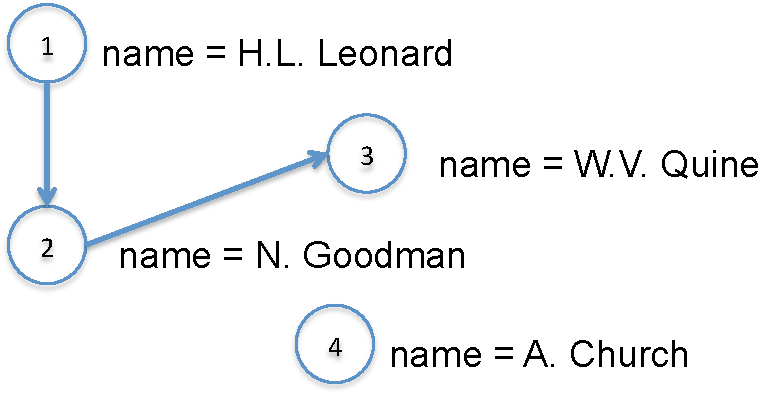
\includegraphics[width=3.2in]{figs/snapshot.pdf}
\caption{Snapshot of DBLP co-authorship graph for 1940, with a single
  string node attribute $name$ and no edge attributes.}
\label{fig:sg}
\end{figure}

Attributes of vertices and of edges are not restricted to be of atomic
types, but may, e.g., be maps or tuples. However it is required that
all vertices (resp. edges) of $G$ have the same schema, i.e., $V$ and
$E$ are homogeneous sets.

\begin{definition} [Structural union-compatibility]
Snapshot graphs $G' = (V', E')$ and $G'' = (V'', E'')$ are
union-compatible if $V'$ and $V''$ are union-compatible, and $E'$ and
$E''$ are union-compatible.
\label{def:scompat}
\end{definition}

This is the standard union compatibility definition, which requires
that vertex schema $V$ and edge schema $E$ be the same for $G'$ and
$G''$.  For example, the snapshot in Figure~\ref{fig:sg} is only
compatible with other snapshots where vertices have one non-key string
attribute $name$ and no non-key edge attributes.

$G$ may represent a directed or an undirected graph.  For undirected
graphs we choose a canonical representation of an edge, with $vid_1
\leq vid_2$ (self-loops are allowed).

We next describe how time is represented in our model.  Following the
SQL:2011 standard~\cite{DBLP:journals/sigmod/KulkarniM12}, we adopt
the {\em closed-open} period model, where a period represents all
times starting from and including the start time, continuing to but
excluding the end time.

\begin{definition}[Time period]
A {\em time period} \\$p = [start, end)$ is an interval on the timeline,
  subject to the constraint $start < end$.  We refer to the length of
  time covered by $p$ as its {\em resolution}.
\label{def:period} 
\end{definition}

Unless otherwise noted, we take {\em day} to be the unit of time.
However, sometimes we will work with time periods where {\em month} or
{\em year} are the units of time.  Unit of time will be stated
explicitly where not clear from context.  Examples of time periods are
$p_1=[\tpy{2000},\tpy{2001})$ (a 1-year period),
  $p_2=[\tpym{2000}{12},\tpym{2001}{03})$ (a 3-month period) and
    $p_2=[\tpymd{2000}{12}{01},\tpymd{2001}{03}{01})$ (an 90-day period).

We focus on {\em valid time}, represented by {\em application-time
  period} in SQL:2011 --- the time period during which data is
regarded as correctly reflecting reality.  This is in contrast to {\em
  transaction time} (or {\em system-time period}), which refers to the
time period during which a row is committed to the database.  Our goal
in this work is to support complex analytics over evolving graphs,
under the assumption that all historical data is available in the
database and is read-only.

We represent graph evolution by associating a sequence of snapshots,
which are not themselves time-aware, with a a sequence of time
periods.  This is stated formally next.

\begin{definition} [Temporal Sequence]
A {\em temporal sequence} $P = (p_1, \ldots, p_n)$ is a
sequence of consecutive non-overlapping time periods of the same
resolution, with no gaps.  That is,

\begin{enumerate}
\item $\forall i < n, p_i.end = p_{i+1}.start$, and 
\item $\forall i, j, p_i.end - p_i.start = p_j.end - p_j.start$.
\end{enumerate}
\label{def:tseq} 
\end{definition}

$P$ may be equivalently described by any 2 of the following 3 values:
the start of the earliest period $P.start = p_1.start$, the end of the
latest period $P.end = p_n.end$, and the resolution of any period
$P.res = p_1.end - p_1.start$. For convenience, we refer to the number
of periods in the sequence as $P.size$.

For example, $P=([\tpy{1940},\tpy{1945}), \ldots,
  [\tpy{2010},\tpy{2015}))$ represents a temporal sequence with
    $P.start=\tpy{1940}$, $P.end=\tpy{2015}$, $P.res=5$ years, and
    $P.size=15$.

A special sequence $P^{\epsilon}$ is the null sequence, with
$P^{\epsilon}.res=null$, $P^{\epsilon}.start=null$,
$P^{\epsilon}.end=null$, and  $P^{\epsilon}.size=0$.

\eat{\vera{According to the wiki, $[a,a)$ is considered an empty
      set. So if we just follow the standard interval math semantics,
      we can say: A null temporal sequence is a sequence represented
      by the $[p.start,p.end)$ time interval regardless of the
        resolution. By definition it is of size 0.}}

We next define union-compatibility for temporal sequences, and present
two basic operations on temporal sequences, which we will use as
building blocks when we define our query language in
Section~\ref{sec:lang}.

\begin{definition} [Temporal Union-Compatibility]
Temporal sequences $P'$ and $P''$ are union-compatible if they have
the same resolution, and if we can construct a valid temporal sequence
$P$ with $P.start = min(P'.start, P''.start)$, $P.end = max(P'.end,
P''.end)$, and $P.res = P'.res$.  $P^{\epsilon}$ is union-compatible
with any temporal sequence.
\label{def:tcompat} 
\end{definition}

\begin{example}
Consider the following time sequences, with year as the unit of time.
\begin{itemize}
\item $P_1=([\tpy{2001},\tpy{2003}),[\tpy{2003},\tpy{2005}))$
\item $P_2=([\tpy{2009},\tpy{2010}),[\tpy{2010},\tpy{2011}))$
\item $P_3=([\tpy{2008},\tpy{2010}),[\tpy{2010},\tpy{2012}),[\tpy{2012},\tpy{2014}))$
\item $P_4=([\tpy{2012},\tpy{2014}),[\tpy{2014},\tpy{2016}))$
\item $P_5=([\tpy{2020},\tpy{2022}))$
\end{itemize}

$P_1$ and $P_2$ are not union-compatible because $P_1.res=2$, while
$P_2.res = 1$.  $P_1$ and $P_3$ are not union-compatible because,
while $P_1.res = P_3.res = 2$, it is not possible to construct a valid
temporal sequence with $P.start=1$, $P.end=14$ and $P.res=2$.
Finally, $P_3$, $P_4$ and $P_5$ are pair-wise union-compatible.  As
our example illustrates, a pair of union-compatible sequences may or
may not overlap, and may not even be consecutive.
\label{ex:ex1}
\end{example}

\begin{definition} [Temporal Intersection]
Intersection of union-compatible sequences $P'$ and $P''$, denoted $P'
\cap P''$, is a time sequence $P$, containing intervals that are in
common to $P'$ and $P''$.  If no intervals are in common to $P'$ and
$P''$, this operation returns $P^{\epsilon}$.
\label{def:tseqand}
\end{definition}

Continuing with Example~\ref{ex:ex1}, $P_3 \cap P_4 =
([\tpy{2012},\tpy{2014}))$ and $P_3 \cap P_5 = P^{\epsilon}$.

\begin{definition} [Temporal Union]
Temporal union of union-compatible sequences $P'$ and $P''$, denoted
$P' \cup P''$, is the sequence $P$ with $P.start = min(P'.start,
P''.start)$, $P.end = max(P'.end, P''.end)$, and $P.res = P'.res$.
\label{def:tseqor}
\end{definition}

Note that $P.size \geq P'.size + P''.size$. In Example~\ref{ex:ex1},
$P_3 \cup P_4 =
([\tpy{2008},\tpy{2010}),\ldots,[\tpy{2014},\tpy{2016}))$ and $P_3
    \cup P_5 = ([\tpy{2008},\tpy{2010}), \ldots,
      [\tpy{2020},\tpy{2022}))$.

Recall that a snapshot represents a single state of an evolving graph,
and is not itself time-aware.  Temporal evolution of a graph is
represented by a sequence of snapshots, called {\em temporal graphs}
in our formalism.

\begin{definition} [TGraph]
A {\em temporal graph} (or a {\em \tg}) $T = (G_1, \ldots, G_n; P)$
  associates a sequence of $n$ structurally union-compatible snapshots
  with a temporal sequence $P$, such that $P.size = n$.
\label{def:tgraph} 
\end{definition}

Snapshot graphs in the sequence define the {\em structural schema} of
$T$, while $P$ specifies the {\em temporal schema} of $T$.

Importantly, identity of a vertex persists across snapshots in a
\tg, and across \tgs.  For example, in Figure~\ref{fig:tgraph}
vertex with id 3 represents the same author W. V. Quine, who published
both in 1940 and in 1952.

\begin{figure}
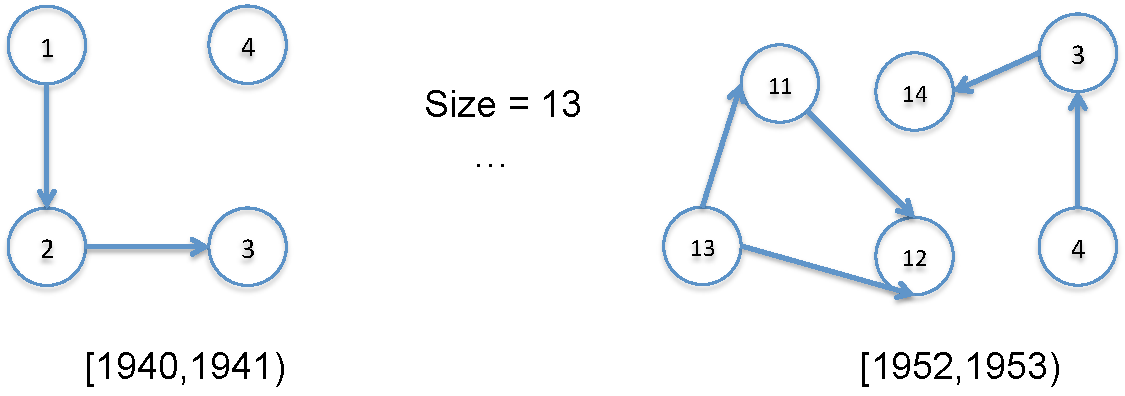
\includegraphics[width=3.2in]{figs/temporalgraph.pdf}
\caption{A \tg of VLDB co-authorship over the period from \tpy{1940} to \tpy{1953}.}
\label{fig:tgraph}
\end{figure}

\julia{Please make Figure~\ref{fig:tgraph} more concrete, list names
  of people as node attributes in addition to, or instead of, ids.
  Also, let's extend this example, so we can use it motivate our
  langauge in the intro, and to illustrate query language predicates.}

To conclude this section, we define union-compatibility for \tgs.

\begin{definition} [\tg Union-Compatibility]
\label{def:tuc} 
$T'$ and $T''$ are union-compatible \tgs if they are both structurally
union-compatible (per Definition~\ref{def:scompat}) and temporally
union-compatible (per Definition~\ref{def:tcompat}).
\end{definition}

The \tg of Definition~\ref{def:tgraph} is the basic element in our
model.  In what follows, we assume that a relation in our database
corresponds to a single \tg, not to a collection of \tgs.  In the next
section we will define the temporal graph query language \ql, in which
operators take as input a single \tg or a pair of \tgs, and produce a
\tg as output.





\section{Algebra}
\label{sec:algebra}
\setlength{\textfloatsep}{5pt}% Remove \textfloatsep

\tg algebra, or \tga for short, is compositional: operators take a \tg
or a pair of \tgs as input, and output a \tg.  We specify the
semantics of \tga by showing a translation of each operator into a
sequence of temporal relational algebra (\tra) expressions (with
nesting, to accommodate non-1NF vertex/edge attributes).  Using this
translation one can implement \tga in a temporal DBMS, guaranteeing
snapshot reducibility and extended snapshot
reducibility~\cite{DBLP:reference/db/Bohlen092} --- two properties
that are appropriate for a point-based temporal data model.

\julia{TRA refresher: time as data, RA operations implicitly handle
  time (snapshot reducibility), explicit reference to time are
  supported in the predicates (extended snapshot reducibility), but
  time cannot be ``created''.}

\julia{Explain temporal subset}

In Section~\ref{sec:algebra:integrity} we present the primitives that
are needed to enforce soundness of \tga.  Then, in
Sections~\ref{sec:algebra:unary} through~\ref{sec:algebra:ecreate}, we
present \tga operators.  Section~\ref{sec:analytics} presents an
extension of \tga to support Pregel-style analytics.  We conclude by
showing expressiveness of \tga in Section~\ref{sec:algebra:formal}.

\subsection{Soundness}
\label{sec:algebra:integrity}

\tga operators are translated into a sequence of expressions in
temporal relational algebra (\tra).  Since TRA is applied to
individual relations of \tve, we must ensure that the combined state
of these relations in the result corresponds to a valid \tg, i.e.,
that the translation is sound.  Recall from Definition~\ref{def:tg}
that a valid \tg must satisfy four requirements: {\bf R1}: Unique
vertices and edges, {\bf R2}: Unique attribute values, {\bf R3}:
Referential integrity, and {\bf R4}: Coalesced.  We now describe three
primitives that will ensure soundness of \tga.

{\bf Coalesce.} To enforce requirements {\bf R1} and {\bf R4}, we
introduce the coalesce primitive $\coal{R}$, which merges adjacent or
overlapping time periods for value-equivalent tuples.  This operation
is similar to duplicate elimination in conventional databases, and has
been extensively studied in the
literature~\cite{DBLP:conf/vldb/BohlenSS96,DBLP:journals/sigmod/Zimanyi06}.
$\coal{R}$ is applied to individual relations of \tve following the
application of operations that uncoalesce.  That the coalesce
primitive can be implemented in relational
algebra~\cite{DBLP:conf/vldb/BohlenSS96}.  Note that eager coalescing
is not always desirable, since it is expensive and some operations may
produce correct results (up to coalescing) even when computing over
uncoalesced inputs~\cite{DBLP:reference/db/Bohlen09}.  Finally, if a
DBMS supports automatic coalescing, this primitive is not necessary.

{\bf Resolve.} To enforce {\bf R2} we introduce the resolve primitive
$\resolve{f_1(k_1), \ldots, f_n(k_n)}{R}$, which is invoked by
operations that produce attribute relations with duplicates.  Resolve
computes a temporal group-by of the attribute relation $\mathbf{R}$ by
key (e.g., by $v$ if $\mathbf{R}$ represents vertex attributes).  It
then computes a bag-union of the properties occurring in each group,
groups together key-value pairs that correspond to the same property
name $\mathbf{k_i}$, and aggregates values within each group using
the specified aggregation function $\mathbf{f_i}$.  If no aggregation
function is specified for a particular property name, \insql{set} is
used as the default.  For example, \julia{example: text or small
  figure}.

{\bf Constrain.} To enforce {\bf R3} we introduce the constrain
primitive $\constr{r}{s}$, which enforces referential integrity on
relation $\mathbf{r}$ with respect to relation $\mathbf{s}$.  For
example, this primitive is used to remove edges from \te for which one
or both vertices are absent from \tv, or validity period of an edge to
be within the validity periods of its vertices.

\eat{The reduce function may, for example, pick the left, the right,
  or an arbitrary element, compute the value of an aggregate function
  such as $\mathbf{COUNT}$, or accumulate values into a set.  A reduce
  function can be repeatedly applied to an unordered collection of
  values to compute a single value, as is done in the map-reduce
  model.  The property graph model allows for arbitrary properties to
  be associated with the graph entities, so it may be impractical or
  infeasible to have the user specify a reduce function for each
  possible property.  In \ql a default reduce function \insql{set} is
  used for any property without an explicitly stated reduction.}

\eat{\begin{lemma}
Let $\psi$ be an n-ary temporal operator on \tg.  If $\psi^T (\ttt)$
produces multiple possible attribute values for any entity at the same
time instant, it must also specify a resolve function for each
property to compute a single valid attribute value.
\end{lemma}}

\eat{In operator definitions below we note which operators are known to
uncoalesce the output, thus requiring coalescing, require FK
enforcement, or include reduce functions.  All non-trivial proofs are
listed in Appendix~\ref{sec:app1}.}

\subsection{Unary operators}
\label{sec:algebra:unary}

\paragraph*{Slice}  The slice operator, denoted $\slice{\bc}{\ttt}$, where
$\bc$ is a time interval, cuts a temporal slice from \ttt. The
resulting \tg will contain vertices and edges whose period $\bp$ has a
non-empty intersection with $\bc$.  We translate this \tga operator to
TRA statements over each constituent relation of \tve:
$\slice{\bc}{\tv}$ and similarly for \te, \tav and \tae.

%: $\slice{\bc}{\tv} = \{ (v, \bp \cap \bc)~~|~~(v, \bp) \in \tv
%\wedge (\pred{\bc}{overlaps}{\bp} \vee \pred{\bc}{contains}{\bp})
%\}$, and analogously for each \te, \tav and \tae.  apply select
%operator to each of the four constituent relations of \tve: $\forall
%x \in \{\tv,\te,\tav,\tae \}, x' = \pi_{A,p \cap c}(\sigma_{p \cap c}
%(x))$, where $A$ is the non-temporal schema of $x$.

\eat{If $p.start < c.start$ or $p.end > c.end$ for some tuple $(g,
  p)$, then $p$ is trimmed to be within the boundaries of $c$: $\tau_c
  (\trg) = \{ (g, p \cap c)~~|~~(g, p) \in \trg \wedge
  (\pred{c}{overlaps}{p} \vee \pred{c}{contains}{p})\}$.  }

Slice does not violate any of the soundness requirements {\bf R1} ---
{\bf R4}, see Appendix~\ref{sec:app1} for proofs of this and similar
statements.

\paragraph*{Subgraph}  Temporal subgraph matching is a generalization of
subgraph matching for non-temporal graphs~\cite{Wood2012}.  This query
comes in two variants.

\eat{A temporal vertex-subgraph query $q^T_v(\tve)$ is a conjunctive query
that takes $\tve (\tv, \te, \tav, \tae)$ as input, and outputs
$\tve'$, an induced temporal subgraph of \tve in which vertices are
defined by $q^T_v$.}

Temporal vertex-subgraph \subv{q^t_v}{\ttt} computes an induced
subgraph of \tve, with vertices defined by the temporal conjunctive
query (TCQ) $q^t_v$.  Note that this is a subgraph query, and so no
new vertices are created, i.e., $\tv' \subseteq^T \tv$.
%As long as $q$ is a valid TCQ that returns a subset of vertex ids
%from \tv, the output is guaranteed to be a valid \tg.

\eat{A temporal edge-sugraph query $q^t_e(\tve)$ is a conjunctive query
that takes a graph $\tve (\tv, \te, \tav, \tae)$ as input, and outputs
a \tg $\tve'$ on the vertices of $\tve$ such that the edges of $\tve'$
are defined by $q^t_e$. }

Temporal edge-subgraph \sube{q^t_e}{\ttt} outputs a subgraph of \ttt,
where edges are defined by TCQ $q^t_e$.  Since this is a subgraph
query, no new edges are created, i.e., $\te' \subseteq^T \te$.

Queries $q^t_v$ and $q^t_e$ may use any of the constituent relations
of \tve to compute the vertex/edge sets.  Further, since these
are TRA queries, they may explicitly reference temporal information,
and so require all input relations to be
coalesced~\cite{DBLP:reference/db/Bohlen09}.

Following the computation of $\tv' = q^t_v(\tv)$, \subv{q^t_v}{\ttt}
must invoke $\coal{\tv'}$ to enforce {\bf R1} and {\bf R4}; and
$\constr{\te'}{\tv'}$, $\constr{\tav'}{\tv'}$, $\constr{\tae'}{\te'}$
to enforce {\bf R3}.
%
Following the computation $\te' = q^t_e(\te)$, \subv{q^t_e}{\ttt} must
invoke $\coal{\te'}$ to enforce {\bf R1} and {\bf R4}; and
$\constr{\tae'}{\te'}$ to enforce {\bf R3}.  %No further
%validation is required, provided that $q^t_e$ outputs a temporal
%subset of \te.% (see Appendix~\ref{sec:app1}).

\eat{We focus on functions that can be expressed as a pair of {\em
  conjunctive queries} $\sigma_{C_V,C_E} (\ttt)$, where $C_V$
specifies a predicate over the vertices and $C_E$ --- over the
vertex-edge triplets.  The predicates can be over the attributes, ids,
and the timestamps of the vertices and edges.  We allow predicates
over the timestamps to support extended snapshot reducibility.
Computing arbitrary subgraphs with path expressions is beyond the
scope of this paper, and we defer this to future work.}

\eat{
$\sigma_{C_V,C_E} (\ttt) = (\tv',\te',\tav',\tae') ~|~$ \\
$\tv' = \pi_{v,p} (\sigma_{C_V} ( \tv \bowtie^T_v \tav))$ \\
$\te' = \pi_{v_1,v_2,p} (\sigma_{C_E} ( \tae \bowtie^T_{v_1} \tav \bowtie^T_{v_2} \tav))$ \\
$\tav' = \sigma_{C_V} (\tav)$ \\
$\tae' = \pi_{v_1,v_2,a} (\sigma_{C_E} (\tae \bowtie^T_{v_1} \tav \bowtie^T_{v_2} \tav))$}

\eat{ Note that as B{\"{o}}hlen showed
  in~\cite{DBLP:reference/db/Bohlen09}, correctness of a select
  operator with a temporal predicate depends on the coalesced state of
  the relation.  When composing a triplet, we carry the vertex and
  edge timestamps in their entirety as data to produce correct
  results.}

% There is no need for an example here, it is clear what these queries
% compute.

\eat{Because we allow predicates over the triplets, interesting conditions
can be expressed.  For example, we can filter out any edges where the
value of some property of its two vertices does not match.  Assuming
vertices have property \insql{group}, we can compute
$\sigma_{T,v1.a.group=v2.a.group}(\ttt)$.}

\eat{
Vertex-subgraph: {\bf R1,R2}: coalesce $\tv'$; {\bf R3}: enforce FK on
$\tav', \te', \tae'$. Edge-subgraph: {\bf R1,R2}: coalesce $\te'$;
{\bf R3}: enforce FK on $\te'$ and $\tae'$.}

\eat{Vertex-subgraph requires coalescing of $\tv'$ and FK enforcement on
\tav', \te', and \tae'. Edge-subgraph requires coalescing of $\te'$ and
FK enforcement on \tae'.}

%\subsection{Temporal map}
%\label{sec:algebra:project}

\paragraph*{Map}  Temporal vertex-map and edge-map apply
user-defined map functions $f_v$ and $f_e$ to vertex or edge
attributes.  Temporal vertex-map $\vmap{f_v, \tve}$ outputs $\tve'$ in
which $\tv'=\tv$, $\te'=\te$, $\tae' = \tae$, and $\tav' =
\pi_{v,f_v(a)}\tav$. Temporal edge-map $\emap{f_e, \tve}$ is defined
analogously.

\eat{To evaluate $\map_{M_V,M_E} (\tve)$, we set $\tv'=\tv$ and $\te'=\te$,
and compute $\tav' = \map_{M_V}(\tav)$ and $\tae' = \map_{M_E}(\tae)$.}

\eat{Temporal map iterates over the tuples of \trg, and applies the
user-specified map functions $M_V$ and $M_E$ to the vertices and edges
of each $g$: $\map_{M_V,M_E} (\trg) = \{(g', p)~~|~~(g,p) \in \trg
\wedge g'= \map_{M_V,M_E}(g)\}$.
}  

While $f_v$ and $f_e$ are arbitrary user-specified functions, there
are some common cases.  Map may specify the set of properties to
project out or retain, it may aggregate (e.g., \insql{COUNT}) or
deduplicate values of a collection property, or flatten a nested
value.

To produce a valid \tg, $\vmap{f_v, \tve}$ must invoke $\coal{\tv'}$
and $\emap{f_e, \tve}$ must invoke $\coal{\te'}$, enforcing {\bf R4}.

% because this is an arbitrary operation, we don't need to invent
% syntax here.  it's also clear what this operation does, I don't
% think there is a need for an example.

\eat{In such cases we will use short-hand
notation similar to projection, listing the properties that we wish to
retain. For example, $\map_{M_V:{school},M_E:\emptyset} (\insql{T1})$
will keep only the school property of the vertices, and no properties
of the edges.  Another useful map operation eliminates duplicates in
the bag of a particular vertex or edge property.  \eat{It may also be
useful to flatten nested bags or aggregate multiple values of the same
property of a vertex or edge, e.g., compute a sum or an average
following temporal intersection or union
(Section~\ref{sec:algebra:join}).}}

%Vertex-map: {\bf R2}: coalesce $\tav'$.  Edge-map: {\bf R2}: coalesce
%$\tae'$.

\eat{Vertex-map requires only coalescing of $\tav'$. Edge-map requires
  only coalescing of $\tae'$.}

\subsection{Aggregation}
\label{sec:algebra:agg}

Aggregation is a common graph operation that computes the value of a
vertex property $pname$ based on information available at the vertex
itself, at the edges associated with the vertex, and at its immediate
neighbors.  Aggregation that can be used to compute simple properties
such as in-degree of a vertex, or more complex ones such as the set of
countries in which the friends of $v_1$ live.

It is convenient to think of aggregation as operating over a temporal
view $L(v_1,v_2,v_1.a,v_2.a,e.a,p)$, where $v_1$ refers to the vertex
for which the new property is being computed, $v_2$ refers to the
vertex from which information is gathered, $v_1.a$, $v_2.a$ and $e.a$
are attributes of the vertices and of the edge, and $p$ is the
associated time period.  $L$ is computed with a temporal join of \te
with two copies of \tv, one for each side of the edge, and with $\tav$
and $\tae$ outer-joined with the corresponding relations.  The
outer-join is needed because a vertex / edge is not required to
specify an attribute.  When \tve represents a directed graph, and
direction of the edge is important for aggregation, it can be
accounted for in the way the join is set up (e.g., mapping $v_2$ in
\tae to $v_1$ in $L$ if the goal is to aggregate information on
incoming edges).

Aggregation is denoted $\insql{agg}^T(dir,cond,f_m,f_a,\ttt)$, where
$dir$ is the direction of the edge (one of 'right', 'left' or 'both')
that determines how $L$ is computed, $cond$ is a predicate over $L$,
$f_m$ is a map function that emits a value for each tuple in the
result of $\sigma^T_{cond}(L)$ (e.g., 1 for computung degree of $v_1$,
or $v_2.a.country$ for computing the set of countries in which the
friends of $v_1$ live).  Finally, $f_a$ is the function that
aggregates values computed by $f_m$.  Putting everything together, and
omitting the computation of $L$ for clarity: we compute a temporal
relation $R = v_1 \gamma^T_{f_a} (\pi_{v_1,f_m} (\sigma^T_{cond} L))$.
As the final step, $\tav' = \coal{\pi_{v, \tav.a \cup R.a} (\tav
  \rightouterjoin^T_{v=v_1} R)}$.

\eat{The result is a new isomorphic graph $\ttt'$:
$\agg{cond,msg,red}{\ttt} = \{ \tv, \te, \tav', \tae \}$, where $\tav'
= \pi^T_{v,a_1+a_2}(\tav \bowtie^T_v$ $_v\vartheta^T_{f} (msg
(\sigma_{cond} (\tae \bowtie^T_{v_1} \tav \bowtie^T_{v_2} \tav))))$.
The temporal join is used to add the new properties to the output
since it may have different periods of validity.  For example, while
each vertex in \tg may remain unchanged for the whole duration,
aggregating vertex degrees would result in an attribute value for each
period of topology change.}

The default aggregation functions $f_a$ is \insql{set}.  We support
various aggregation functions $f_a$, including the standard \{
\insql{count} | \insql{min} | \insql{max} | \insql{sum} \}, which have
their customary meaning.  We also support \{ \insql{any} |
\insql{first} | \insql{last} | \insql{set} | \insql{list} \}, which
are possible to compute because properties being reduced have temporal
information.  \insql{first} and \insql{last} refer to the value of a
property with the earliest/latest timestamp, while \insql{set} and
\insql{list} associate a key with a collection of values.

\eat{As an example, to compute vertex in-degrees, we can use
  $\agg{msg=(dst,p,1),red=count}{\ttt}$.  To compute a set of places
  that all close friends have visited in the past year, assuming there
  is a property \insql{places} on friend vertices and closeness of
  friendship property on edges:\\ $\agg{cond=dst.p \cap [2015,2016) \&
      a.close > 0.8,msg=(src,p,dst.places)}{\ttt}$.}

%To produce a valid \tg, \insql{agg} must invoke \coal{\tav'}.
\julia{I don't think so: {\bf R2}: require reduce function.}

\subsection{Binary set operators}
\label{sec:algebra:binary}

We support the temporal versions of the three binary set operators
intersection ($\cap^T$), union ($\cup^T$), and difference
($\setminus^T$).  As Dignos et al. showed, the three set operators are
not schema robust~\cite{Dignos2012}.  Schema robust operators are not
affected if the argument relation is extended by an additional
attribute.  This presents a problem when executing the set operations
over the \tav and \tae relations as there is no guarantee that a
vertex or an edge with the same identity and at the same time instant
has the same attribute set.  Thus all three operators that the resolve
primitive be invoked as the last step.

Let $\oplus$ be a temporal set operator $\in \{ \cap^T, \cup^T,
\setminus^T \}$ and $f_v$ and $f_e$ represent aggregate functions for
vertex and edge attributes, respectively.  We compute $\oplus$ by
computing:\\ $\tv' = \tv_1 \oplus \tv_2$, $\te' = \te_1 \oplus \te_2$,\\
$\tav' = \constr{\resolve{f_v}{\tav_1 \fullouterjoin^T_{v} \tav_2}}{\tv'}$,\\
$\tae' = \constr{\resolve{f_e}{\tae_1 \fullouterjoin^T_{v1,v2} \tae_2}}{\te'}$.

Note that $\tav'$ and $\tae'$ are constrained w.r.t. $\tv'$ and
$\te'$, respectively, in the expressions above.

 \eat{Then $\tve_1 \oplus_{f_v,f_e} \tve_2 = \{ \tv_1 \oplus \tv_2,
   \te_1 \oplus \te_2, \pi^T_{v,red(a_1,a_2)}(\tav_1
   \fullouterjoin^T_{v}
   \tav_2),$\\ $\pi^T_{v_1,v_2,red(a_1,a_2)}(\tae_1
   \fullouterjoin^T_{v_1,v_2} \tae_2) \}$, with all FK constraints on
   \tav and \tae enforced.}

\eat{As elsewhere, the default reduce function is \insql{set}.  In addition
to the functions defined in Section~\ref{sec:algebra:agg} we also
support \{ \insql{left} | \insql{right} \}, which select the attribute
of the left, resp. right, operand.}

%\subsection{Temporal graph intersection}
%\label{sec:algebra:join}
\eat{
The binary temporal graph intersection operation $\trga \cap \trgb$
computes a temporal join~\cite{Gao2005} of \trga and \trgb with the
predicate $\trga.p \cap \trgb.p \neq \emptyset$, producing a tuple for
each pair of representative graphs for which time periods intersect:
$\trga \cap \trgb = \{(g_1 \cap g_2, p_1 \cap p_2)~|~((g_1, p_1) \in
\trga \wedge (g_2, p_2) \in \trgb \wedge p_1 \cap p_2 \neq \emptyset
\}$.  The result of $g_1 \cap g_2$ is computed by intersecting the
sets of vertices and of edges of the graphs~\cite{GraphTheory}.  For
each vertex and edge in the result, we compute a {\em union} of their
bags of properties.% \julia{Figure with example.}
%
Algorithm~\ref{alg:inter} presents the evaluation of $\tvea \cap
\tveb$. We compute temporal joins over \tv and \te (lines 1, 2).  We
then compute \tav' and \tae' with temporal outer joins of the
corresponding relations (lines 3, 4).  Finally, we enforce foreign key
constraints on \te', \tav' and \tae' (lines 5, 6).
}

%\begin{algorithm}[b]
%\caption{Temporal graph intersection in \tve.}
%\begin{algorithmic}[1]
%%\REQUIRE $\tvea (\tv_1;\te_1;\tav_1;\tae_1), \tveb (\tv_2;\te_2;\tav_2;\tae_2)$.\\
%\REQUIRE $\tvea, \tveb$.\\
%\STATE $\tv' = \tv_1 \Join^T_v \tv_2$\\ 
%\STATE $\te' = \te_1 \Join^T_{v_1,v_2} \te_2$\\ 
%\STATE $\tav' = \cl (\pi_{v,p,\tav_1.a \cup \tav_2.a}\tav_1 \fullouterjoin^T_v \tav_2)$\\
%\STATE $\tae' = \cl (\pi_{v_1,v_2,p,\tae_1.a \cup \tae_2.a}\tae_1 \fullouterjoin^T_{v_1,v_2} \tae_2)$\\
%\STATE $\tae' = \pi_{a_1 \cap a_2}(\tae_1 \Join^T \tae_2)$\\
%\STATE enforce foreign keys on $\tav'$ w.r.t. $\tv'$\\ 
%\STATE enforce foreign keys on $\tae'$ w.r.t. $\te'$\\ 
%\RETURN new $\tve (\tv';\te';\tav';\tae')$\\
%\end{algorithmic}
%\label{alg:inter}
%\end{algorithm}

\begin{figure*}
%\centering
\begin{subfigure}{2.5in}
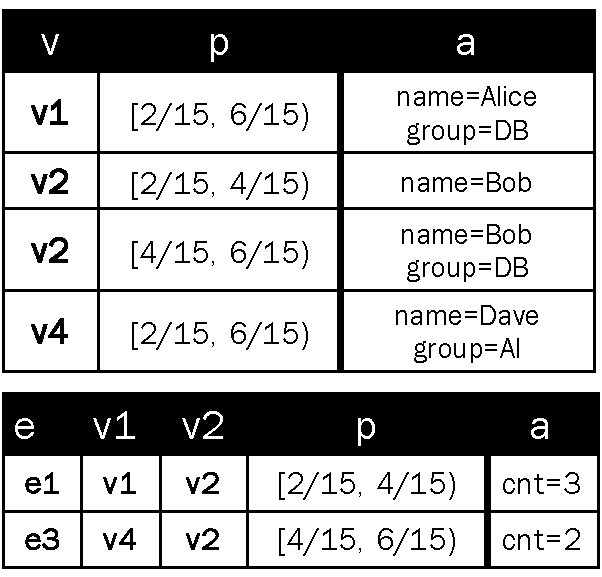
\includegraphics[width=2.5in]{figs/T2_rel.pdf}
\caption{T2.}
\label{fig:tg_t2}
\end{subfigure}
\begin{subfigure}{4.3in}
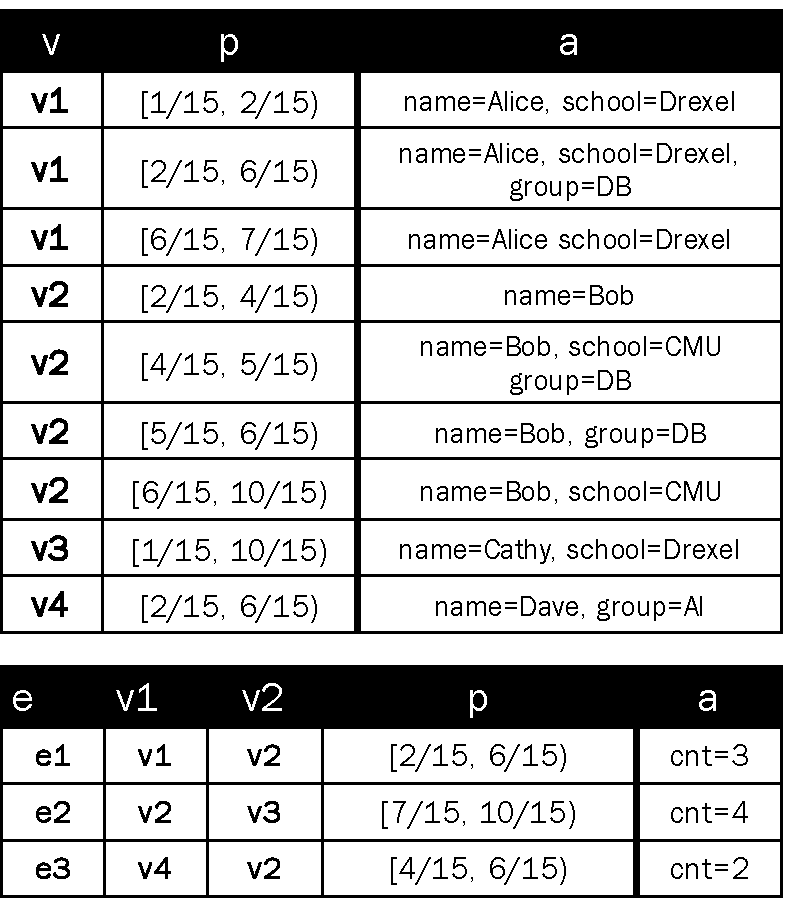
\includegraphics[width=4.3in]{figs/T1_union_T2_rel.pdf}
\caption{$T1 \cup^T T2.$}
\label{fig:tg_union}
\end{subfigure}
\begin{subfigure}{2.3in}
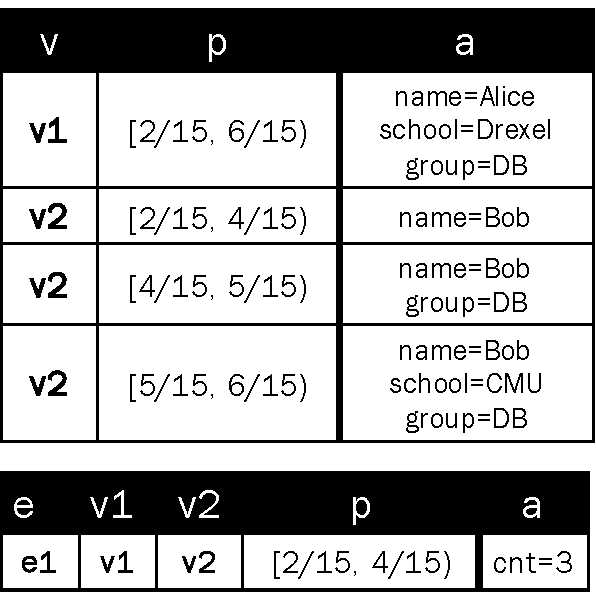
\includegraphics[width=2.3in]{figs/T1_inter_T2_rel.pdf}
\caption{$T1 \cap^T T2$.}
\vspace{-0.2cm}
\label{fig:tg_inter}
\end{subfigure}
\begin{subfigure}{2.3in}
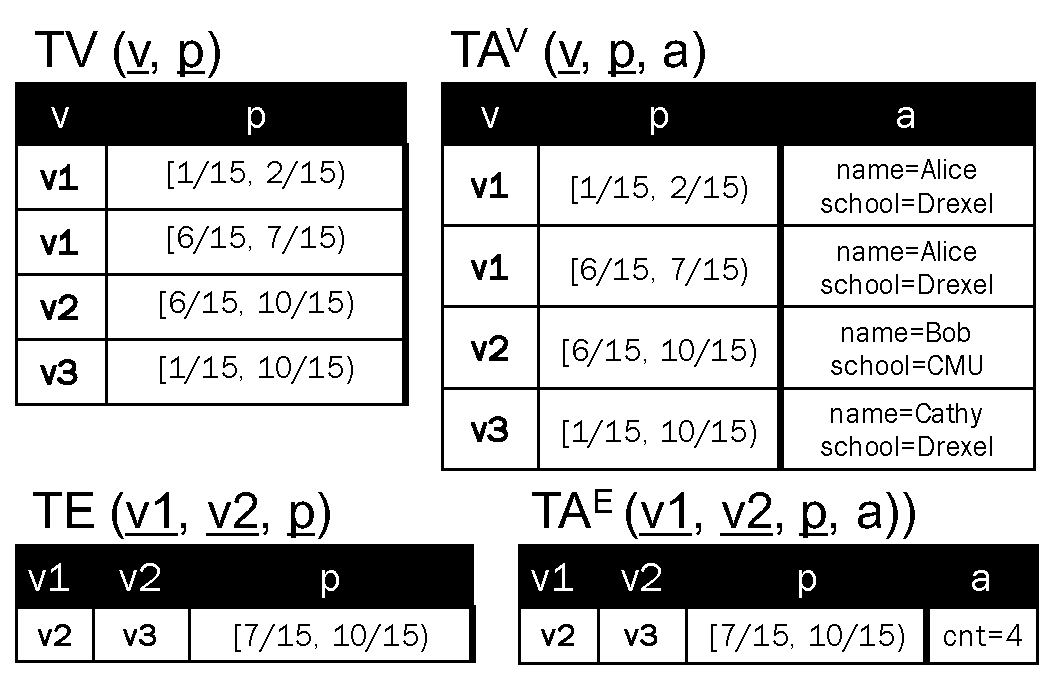
\includegraphics[width=2.3in]{figs/T1_diff_T2_rel.pdf}
\caption{$T1 \setminus^T T2$.}
\vspace{-0.2cm}
\label{fig:tg_diff}
\end{subfigure}
\caption{Binary operators.}
\label{fig:binary}
\vspace{-0.2cm}
\end{figure*}

Consider \insql{T1} in Figure~\ref{fig:tg} and \insql{T2} in
Figure~\ref{fig:tg_t2}.  Figure~\ref{fig:tg_inter} illustrates
\insql{T1} $\cap^T$ \insql{T2}.  Period $[2/15, 4/15)$ for $v_2$ is
  computed as a result of the join of $[2/15, 5/15)$ in T1 and [$2/15,
      4/15)$ in T2.  Only the vertices and edges present in both \tgs
      are produced, thus eliminating $v_3$ and $v_4$.
      Figure~\ref{fig:tg_union} is similar to
      Figure~\ref{fig:tg_inter} but uses temporal union instead of
      intersection.  According to the definition of temporal union,
      periods are split to coincide for any group and thus the
      attribute values for e.g., $v_1$ have three distinct tuples.
      Figure~\ref{fig:tg_diff} shows the result of temporal difference
      of \insql{T1} and \insql{T2}.  Vertex $v_1$ in the result is
      present before $2/15$ and after $6/15$, splitting one $v_1$
      tuple in \tv of \insql{T1} into two temporally-disjoint tuples
      in \tv of the result (and similarly for \tav).

\eat{In addition to invoking reduce on the attribute relations for all
operations, it is required to invoke $\constr{\tav'}{\tv}$ and
$\constr{\tae'}{\te}$ for }

\eat{{\bf R1, R2}: for all set operators coalesce every relation in
$\ttt'$; {\bf R3}: enforce FK on $\tav'$ and $\tae'$ for difference,
intersection. {\bf R4}: require reduce function.}

\eat{Intersection and union may uncoalesce, while difference does not.
  Intersection and difference require FK enforcement for \tav and
  \tae, while union does not.}

%\subsection{Temporal graph union}
%\label{sec:algebra:outerjoin}

\eat{
The binary temporal graph union operation $\trga \cup \trgb$ computes
a temporal full outer join~\cite{Gao2005} of \trga and \trgb on the
predicate $\trga.p \cap \trgb.p $. For tuples $(g_1, p_1) \in \trga$
and $(g_2, p_2) \in \trgb$ for which $p_1 \cap p_2 \neq \emptyset$, we
compute $(g_1 \cup g_2, p_1 \cap p_2)$.  The result of $g_1 \cup g_2$
is computed by taking a {\em union} of the sets of vertices and of
edges of the graphs~\cite{GraphTheory}.  For each vertex and edge in
the result, we compute a {\em union} of their bags of properties.
Tuples from \trga (resp. \trgb) for which there does not exist a tuple
in \trgb (resp. \trga) for part or all of the validity period are
included in the result of the full outer join. 
}

\eat{
 $\trg_1 \cup \trg_2 = \{ (g, p) | (g_1, p_1) \in \trg_1 \wedge (g_2,
p_2) \in \trg_2 \wedge ((g = g_1 \cup g_2 \wedge p = p_1 \cap p_2
\wedge p_1 \cap p_2 \neq \emptyset) \vee (g = g_1 \wedge p = p_1 - p_2
\wedge \nexists p \in \trg_2 = p_1 - p_2) \vee (g = g_2 \wedge p = p_2
- p_1 \wedge \nexists p \in \trg_1 = p_2 - p_1))\}$.  Similar to
temporal intersection, temporal union is essentially an outer
theta-join of $\trg_1$ and $\trg_2$ with a $p_1 \cap p_2$ predicate.
We use the standard graph union definition based on set theory, which
computes unions of the vertex and edge sets from the two
operands~\cite{GraphTheory}.}

\eat{
Algorithm~\ref{alg:union} presents the evaluation of $\tvea \cup
\tveb$.  We compute temporal outer joins over the corresponding \tv,
\te, \tav and \tae.
}

\eat{\begin{algorithm}[t]
\caption{Temporal graph union in \tve.}
\begin{algorithmic}[1]
\REQUIRE $\tvea, \tveb$.\\
\STATE $\tv' = \tv_1 \fullouterjoin^T_v \tv_2$\\
\STATE $\te' = \te_1 \fullouterjoin^T_{v1,v2} \te_2$\\
\STATE $\tav' = \cl (\pi_{v,p,\tav_1.a \cup \tav_2.a}\tav_1 \fullouterjoin^T_v \tav_2)$\\
\STATE $\tae' = \cl (\pi_{v_1,v_2,p,\tae_1.a \cup \tae_2.a}\tae_1 \fullouterjoin^T_{v1,v2} \tae_2)$\\
\RETURN new $\tve (\tv';\te';\tav';\tae')$\\
\end{algorithmic}
\label{alg:union}
\end{algorithm}
}

%\subsection{Temporal graph difference}
%\label{sec:algebra:diff}

\eat{
The binary temporal graph difference operation $\trga \setminus \trgb$
computes a temporal left outer join~\cite{Gao2005} of \trga and \trgb
on the predicate $\trga.p \cap \trgb.p$.  For tuples $(g_1, p_1) \in
\trga$ and $(g_2, p_2) \in \trgb$ for which $p_1 \cap p2 \neq
\emptyset$, we compute $(g_1 \setminus g_2, p_1 \cap p_2)$.  The
result of $g_1 \setminus g_2$ is computed by taking a {\em set
  difference} of the sets of vertices and of edges of the graphs.  For
each vertex and edge in the result, we compute a {\em union} of their
bags of properties.  Tuples in \trga for which there does not exist a
tuple in \trgb for part or all of the validity period are included in
the result of the left outer join.
}
\eat{
Algorithm~\ref{alg:diff} presents the evaluation of $\tvea \setminus
\tveb$.  We compute temporal left outer joins over the corresponding
\tv and \te (lines 1,2).  We then compute $\tav'$ and $\tae'$ with
temporal outer joins of the corresponding relations (lines 3, 4).
Finally, we enforce foreign key constraints on $\te'$, $\tav'$, and
$\tae'$ (lines 5, 6).
}

\eat{\begin{algorithm}[b]
\caption{Temporal graph difference in \tve.}
\begin{algorithmic}[1]
\REQUIRE $\tvea, \tveb$.\\
\STATE $\tv' = \tv_1 \leftouterjoin^T_v \tv_2$\\ 
\STATE $\te' = \te_1 \leftouterjoin^T_{v_1,v_2} \te_2$\\ 
\STATE $\tav' = \cl (\pi_{v,p,\tav_1.a \cup \tav_2.a}\tav_1 \fullouterjoin^T_v \tav_2)$\\
\STATE $\tae' = \cl (\pi_{v_1,v_2,p,\tae_1.a \cup \tae_2.a}\tae_1 \fullouterjoin^T_{v_1,v_2} \tae_2)$\\
\STATE enforce foreign keys on $\tav'$ w.r.t. $\tv'$\\ 
\STATE enforce foreign keys on $\tae'$ w.r.t. $\te'$\\ 
\RETURN new $\tve (\tv';\te';\tav';\tae')$\\
\end{algorithmic}
\label{alg:diff}
\end{algorithm}
}

\subsection{Node creation}
\label{sec:algebra:ncreate}

We argued in the introduction that it is interesting and insightful to
analyze an evolving graph at different levels of granularity.  For
example, the user may want to aggregate multiple consecutive
representative graphs into a single representative graph, coarsening
the granularity, or to predefine temporal resolution and look at the
graph at that scale, irrespective of whether this resolution happens
to be finer or coarse than the natural evolution rate of the graph.
For this, we introduce a node creation operator which is similar to
the {\em moving window temporal aggregation} in temporal relational
algebra.  Our approach is inspired by stream aggregation work
of~\cite{Li2005}, adopted to graphs, and by generalized quantifiers
of~\cite{Hsu1995}.

Node creation is denoted $\ncr{G_V}{W,Q_V,Q_E,red}{\ttt}$,\\ where
$G_V$ are the grouping attributes, $W$ is the window specification,
$Q_V$ and $Q_E$ are vertex and edge quantifiers, and $red$ is the set
of reduce functions.  It produces a consolidated evolving graph with
specific temporal granularity.

{\em Grouping attributes} $G_V$ are vertex properties by which
vertices are grouped into new entities, similar to \insql{GROUP BY}
clause in SQL.  Since node creation requires new identifiers, the
combination of the grouping properties can be used in a mechanism
equivalent to a Skolem function.  The simplest, default grouping
attribute is the $vid$ of the vertex.

{\em Window specification} $W$ is of the form
$n~\{unit|\insql{changes}\}$, where $n$ is an integer, and $unit$ is a
time unit, e.g., $10~min$, $3~years$, or any multiple of the usual
time units.  Window specification of the form $n~\insql{changes}$
defines the window in terms of change over \trg.\eat{ (which may be
  computed from the \tve representation, see
  Section~\ref{sec:model:switch}).}  For example,
$W=3~\insql{changes}$ will aggregate sequences of 3 representative
graphs into 1.  Window boundaries are computed left-to-right, i.e.,
from least to most recent.  The right-most window may correspond to
fewer than $n$ representative graphs from the input.
%
Our window specification by change is similar to slide-by-row window
in stream aggregation~\cite{Li2005}.  Note that, because \tg algebra
is compositional, we do not support node creation with overlapping
windows, because it does not produce a valid \tg.  To see why this is
so, consider applying a sliding window of 3 months range with 1 month
slide to graph \insql{T} in Figure~\ref{fig:tg_rg}.  We would produce
the following tuples for $v_1$: $(v_1, [1/15, 4/15), a_1)$, $(v_1,
  [2/15, 5/15), a_2)$, $(v_1, [3/15, 6/15))$, and so on, which clearly
      violates the temporally coalesced requirement in
      definition~\ref{tg}.

Similar to~\cite{Li2005} we support creation simultaneously by time
and by non-temporal attributes (e.g., vertex properties).  If the
window specification is one change, then the operation devolves into
pure structural reduce or node creation, as classified by
Wood~\cite{Wood2012}.  If the grouping attribute is the vertex $vid$,
then the operation is purely temporal, with no structural aspect.

{\em Quantifiers} $Q_V$ and $Q_E$ are of the form \{ \insql{all} |
\insql{most} | \insql{at least} $n$ | \insql{exists} \}, where $n$ is
a decimal representing the percentage of the time during which an
entity (vertex or edge) existed, relative to the duration of the
window. Note that \insql{exists} is the default quantifier for
vertices and edges.  Quantifiers are useful for producing different
kinds of representative graphs.  For example, to produce
representative graphs with only strong connections over a volatile
evolving graph, we may want to only include vertices that span the
entire time window ($Q_V=\insql{all}$), and edges that span a large
portion of the window ($Q_E=\insql{most}$).
 
The optional reduce functions compute new
values for vertex and edge properties representative of
the whole window, e.g., $any(name), last(school), sum(cnt)$.
%
 
\eat{Key-value pairs for vertex and edge properties for which no
aggregation functions are specified, are collected into a bag
corresponding to the entity in the result.  These can be subsequently
transformed with $map^T$ (Section~\ref{sec:algebra:project}).}

\eat{ 
Temporal aggregation over \tve follows the outline of
Algorithm~\ref{alg:op}, but requires an additional step, and is
revisited in Algorithm~\ref{alg:agg_ve}.
%
}

We compute group periods based on window specification: $P =
\textsf{computePeriods}(W, \tv, \te, \tav, \tae)$.  We use temporal
aggregation and selection to evaluate $Q_V$ on each group in $\tv$:
$\tv' = \sigma_{P,Q_V}( _{G_V}\vartheta^T (\tv \leftouterjoin^T
\tav))$ and similarly for $\te$: $\te' = \sigma_{P,Q_E}(
_{G_V}\vartheta^T (\te \bowtie^T_{v_1=v} \tav \bowtie^T_{v_2=v}
\tav))$.  The edge triplets, obtained through three-way temporal join
of \tae with \tav are required to aggregate edges by $G_V$.  To
compute attribute relations we compute temporal aggregation with the
reduce functions and enforce FK constraints: $\tav' =
~_{G_V}\vartheta^T_{red}(\tav)$, $\tae' =
~_{G_V}\vartheta^T_{red}(\tae \leftouterjoin^T_{v_1=v} \tav
\leftouterjoin^T_{v_2=v})$.

\eat{
Node creation over \trg is computed by first calculating time periods
from $W$ and \trg, and then reducing and combining the representative
graphs directly.
}

\eat{\begin{algorithm}[t!]
\caption{Node creation in \tve.}
\begin{algorithmic}[1]
\REQUIRE \tve (\tv;\te;\tav;\tae), window specification $W$, vertex
quantifier $Q_V$, edge quantifier $Q_E$, vertex aggregate function
$A_V$, vertex aggregate function $A_E$.\\
\STATE $P = \textsf{computePeriods}(W, \tv, \te, \tav, \tae)$\\
\STATE  $\tv' = \cl (_{G_V}\vartheta_{P,Q_V}(\tv))$\\
\STATE  $\te' = \cl (_{G_V}\vartheta_{P,Q_E}(\te))$\\
\STATE  $\tav' = \cl (_{G_V}\vartheta_{P,A_V}(\tav))$\\
\STATE  $\tae' = \cl (_{G_V}\vartheta_{P,A_E}(\tae))$\\
\STATE  follow steps 5-7 of Algorithm~\ref{alg:op}\\
%\STATE  enforce foreign keys on $\te'$ w.r.t. $\tv'$\\
%\STATE  enforce foreign keys on $\tav'$ w.r.t. $\tv'$\\
%\STATE  enforce foreign keys on $\tae'$ w.r.t. $\te'$\\
\RETURN new $\tve (\tv';\te';\tav';\tae')$\\
\end{algorithmic}
\label{alg:agg_ve}
\end{algorithm}
}

Figure~\ref{fig:tg_agg1} illustrates node creation by time
($W=3~\textsf{months}$), and Figure~\ref{fig:tg_agg2} --- by change
($W=3~\textsf{changes}$).  Figure~\ref{fig:tg_agg3} illustrates
structural reduce only ($W=1~\textsf{change}$), and
Figure~\ref{fig:tg_agg4} both structural and temporal
($G_V=\textsf{school}, W=3~\textsf{months}$).  All four are applied to
\insql{T1} in our running example, and list the same quantifiers
(\insql{all} for vertices and \insql{exists} for edges) and reduce
functions (\insql{first} for vertex and edge properties).  $v_2$ is
present in the result in Figure~\ref{fig:tg_agg1} starting at $4/15$
because it did not exist for the entirety of the first window, while
in Figure~\ref{fig:tg_agg2} it is produced starting $6/15$.  In
Figure~\ref{fig:tg_agg3} vertices $v1$ and $v3$ create a single new
vertex $v1$ representing the institution.  A subsequent \insql{map}
operation to produce a new name attribute and a count of people would
produce a more meaningful final result.

\begin{figure*}[t]
%\centering
\begin{subfigure}[b]{0.5\textwidth}
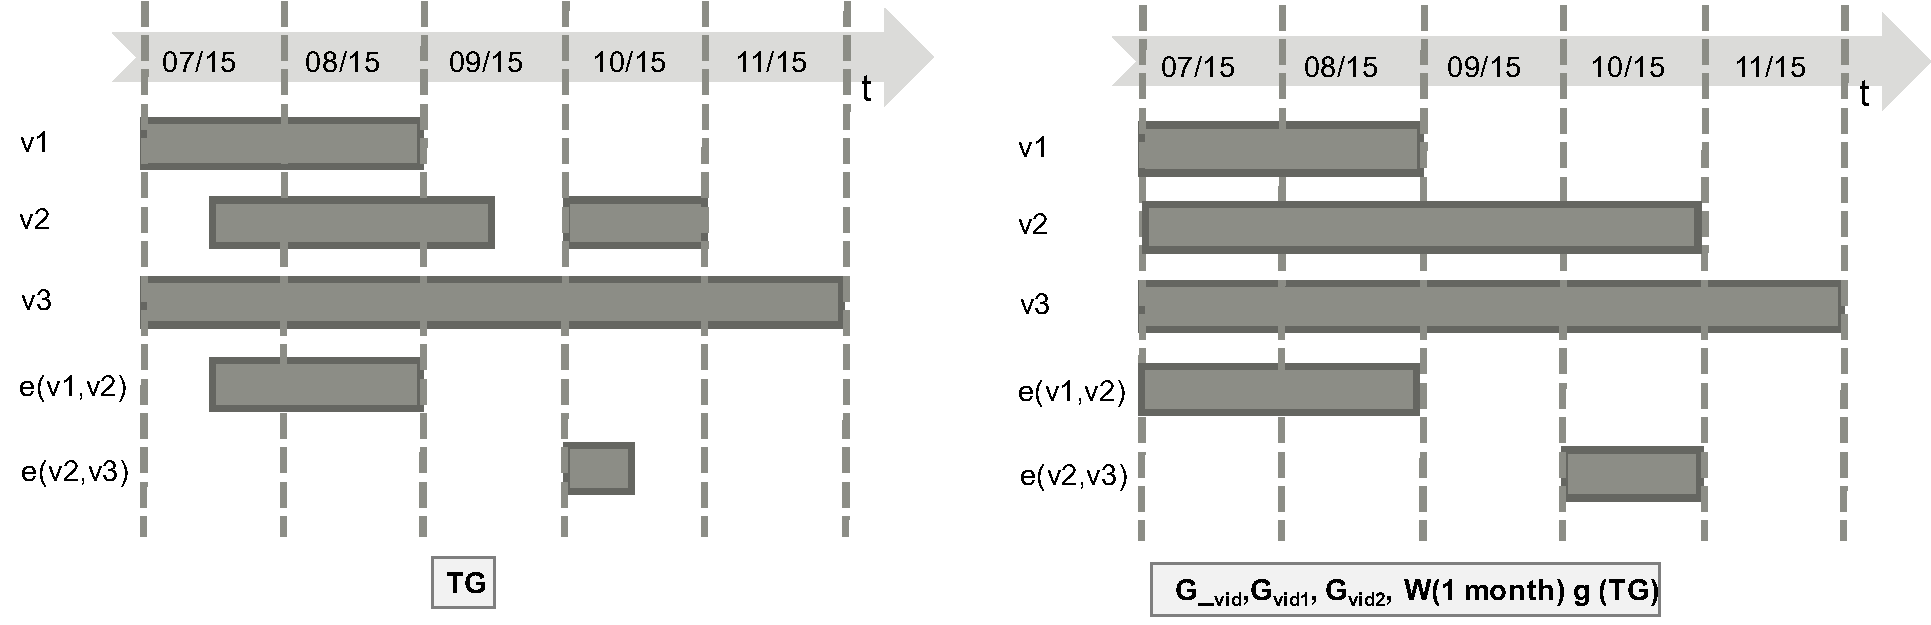
\includegraphics[width=3.2in]{figs/agg1.pdf}
\caption{By time: $W=3~\textsf{months}, G_V=\textsf{vid}$.}
\label{fig:tg_agg1}
\end{subfigure}
\begin{subfigure}[b]{0.5\textwidth}
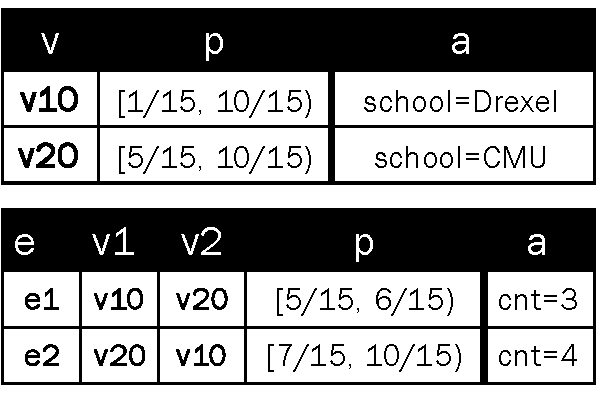
\includegraphics[width=3.2in]{figs/agg3.pdf}
\caption{Grouped by attribute: $W=1~\textsf{change}, G_V=\textsf{school}$.}
\label{fig:tg_agg3}
\end{subfigure}
\begin{subfigure}[b]{0.5\textwidth}
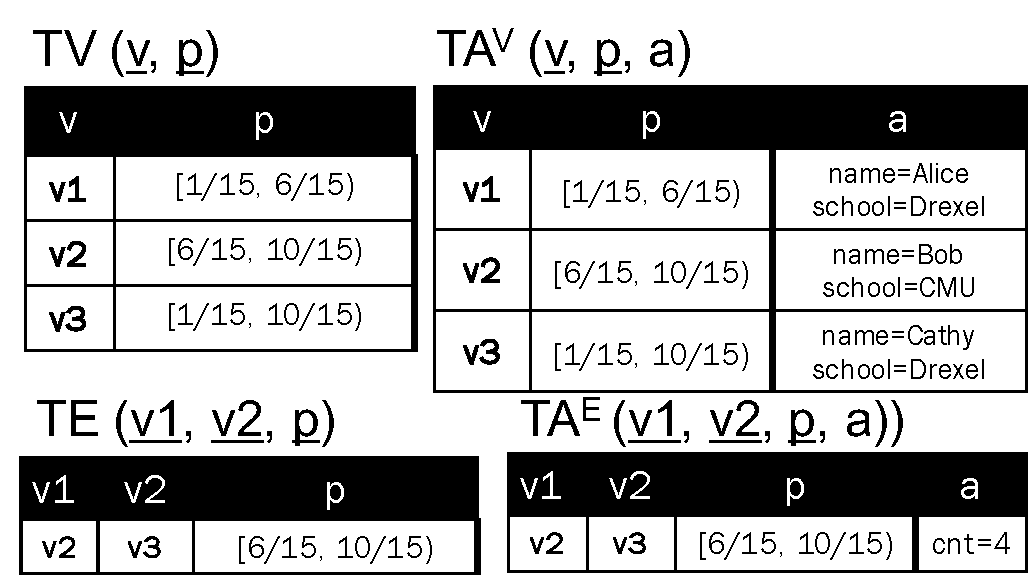
\includegraphics[width=3.2in]{figs/agg2.pdf}
\caption{By change: $W=3~\textsf{changes}, G_V=\textsf{vid}$.}
\label{fig:tg_agg2}
\end{subfigure}
\begin{subfigure}[b]{0.5\textwidth}
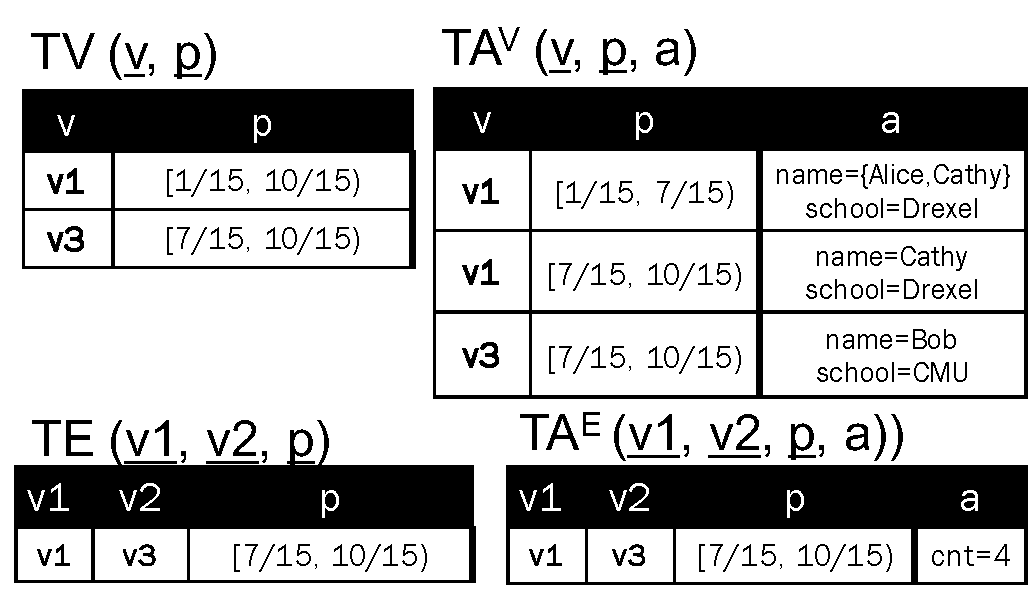
\includegraphics[width=3.2in]{figs/agg4.pdf}
\caption{By time with grouping: $W=3~\textsf{months}, G_V=\textsf{school}$.}
\label{fig:tg_agg4}
\end{subfigure}
\caption[]{Node creation, $Q_V=\insql{all}$, $Q_E=\insql{exists}$,
  $A_V=\insql{first}$, $A_E=\insql{first}.$}
\label{fig:tg_agg}
\vspace{-0.5cm}
\end{figure*}

\eat{Node creation may uncoalesce and requires FK enforcement.}

{\bf R1, R2}: coalesce every relation in $\ttt'$; {\bf R3}: enforce FK
on $\tav', \te', \tae'$; {\bf R4}: require reduce function.

\eat{ Our aggregation quantifiers are inspired by generalized
  quantifiers of~\cite{Hsu1995} with n-place delimiters.  $Q(R)$ as a
  Boolean-valued function of a relation''~\cite{Hsu1995}.  A
  quantifier contains an n-place determiner, e.g., ``at least one
  vertex in each window for each group'' is a 2-place determiner
  quantifier.  \tg algebra supports determiners from the set
  $\{at\ least\ one, all, most, at\ least\ n\}$, where $n$ is an
  integer representing a ratio.  $all$ is a usual universal quantifier
  that in standard SQL can be achieved with the use of two \insql{NOT
    EXISTS}.}

\subsection{Edge creation}
\label{sec:algebra:ecreate}

Edge creation operator outputs a new graph with edges based on the two
input \tgs.  Let $\ecr{\ttt_1}{q,red}{\ttt_2}$ be an edge creation
operator, where $q$ is a conjunctive query over constituent relations
of $\tve_1$ and $\tve_2$ and $red$ is a reduce function. $q$ must
return a valid temporal relation $(v_1, v_2, a_1, a_2)$.  The reduce
function is used to compute the final $\tae'$ relation.
$\ecr{\ttt_1}{q,red}{\ttt_2} = \{ \tv', \te', \tav', \tae' \}$, where
$\tae' = \sigma^T_{v_1,v_2,red(a_1,a_2)}(q(\ttt_1, \ttt_2))$ subject
to FK constraint from $\tv_1 \cup^T \tv_2$, $\te' =
\sigma^T_{v_1,v_2}(\tae')$, \tv' is a subset of $\tv_1 \cup^T \tv_2$
such that it contains only vertices with edges in $\te'$, and $\tav'$
is an empty relation.  Intuitively, edge creation returns a new \tg
from nodes of $\ttt_1$ and $\ttt_2$ with no attributes, connected by
edges determined by $q$.

Edge creation has several important applications.  In graph theory, a
graph join of two undirected unlabeled disjoint graphs is defined as
the union of the two graphs and additional edges connecting every
vertex in graph one with each vertex in graph two.  We can obtain a
graph join by the application of edge creation with $q = $ a temporal
cartesian product of $\tv_1$ and $\tv_2$.
SocialScope~\cite{Amer-Yahia2009} defines a nontemporal graph
composition operator which produces a graph induced by edges that are
composed from edges in the two operands connected by a common vertex
with a directional condition.  In \ql temporal graph composition can
be computed using node creation of \ttt with itself and a $q = $ a
temporal theta-join of $\tae$ and $\tae_2$.  This allows computation
of friend-of-friend edges, which, if applied k times, can answer k-hop
queries.  Since $q$ can include predicates over the timestamps, edge
creation can also compute journeys.  A journey is a path in the
evolving graph with non-decreasing time
edges~\cite{Ferreira2004,Casteigts2011}.  By adding a temporal
condition to the theta-join of $\tae_1$ and $\tae_2$ we can obtain
journeys similar to time-concurrent paths.

\julia{Example of edge transpose goes here.}

Note that edge creation is not additive, it produces {\em new} edges.
To add these edges to the original graph, a subsequent union must be
performed.

\eat{Graph composition operator in our algebra is a temporal extension of
the composition operator in SocialScope~\cite{Amer-Yahia2009}.  It
produces a graph induced by edges that are composed from edges in the
two operands for any time point when they coexisted.  The value of the
new edge attributes is determined by the resolve function, similar to
the set based operators.}

\eat{
Let $\odot_{\delta,r}$ be a composition operator, where $\delta$ is a
directional condition pair $d_1=v_1|v_2, d_2=v_1|v_2$ and $r$ is a
resolve function.  Then $\ttt_1 \odot_{\delta,r} \ttt_2 = \{ \tv',
\te', \tav', \tae' \}$, where $\forall (v_x,v_z,p) \in \te' \exists
(d_1,v_x,p_1) \in \te_1 \wedge (d_2,v_z,p_2) \in \te_2 \wedge p=p_1
\cap p_2$, \tv' contains only vertices with edges in \te', with FK
constraint enforced on \tav' from \tv', and $\forall (v_x,v_z,p,a) \in
\tae' \exists (d_1,v_x,p_1,a_1) \in \tae_1 \wedge (d_2,v_z,p_2) \in
\tae_2 \wedge p=p_1 \cap p_2 \wedge a=r((a_1,p_1),(a_2,p_2))$.
}

\eat{For example, to create edges between vertices that have two degrees of
separation, i.e. friends of friends, we can compose the graph with
itself with $d_1=v_2$ and $d_2=v_2$.  }

{\bf R1, R2}: coalesce $\te'$ and $\tae'$; {\bf R3}: constraint $\te'$
on $\tv'$, $\tv'$ on $\te'$ (to remove nodes with no edges), and
$\tae'$ on $\te'$; {\bf R4}: require reduce function.

\section{Analytics}
\label{sec:analytics}


%\section{Portal by Example}
\label{sec:example}

In this section we present \ql, a declarative query language for
evolving graphs. \ql uses SQL-like syntax, and has the form
\insql{TSelect} \ldots \insql{From} \ldots \insql{TWhere} \ldots
\insql{TGroup}.  We prefix temporal keywords with \insql{T}, to make
the distinction between \ql and SQL operations explicit.  We will use
\tgs \insql{T1} and \insql{T2} of Figures~\ref{fig:tg}
and~\ref{fig:tg_t2}, with structural schema V(\underline{vid}:int,
name:str, salary:int); E(\underline{vid1}:int, \underline{vid2}:int,
cnt:int), in our examples.

\subsection{Portal Basics}
\label{sec:example:basics}

{\bf Temporal selection.}  Consider query $Q1$ below.  

\begin{figure}
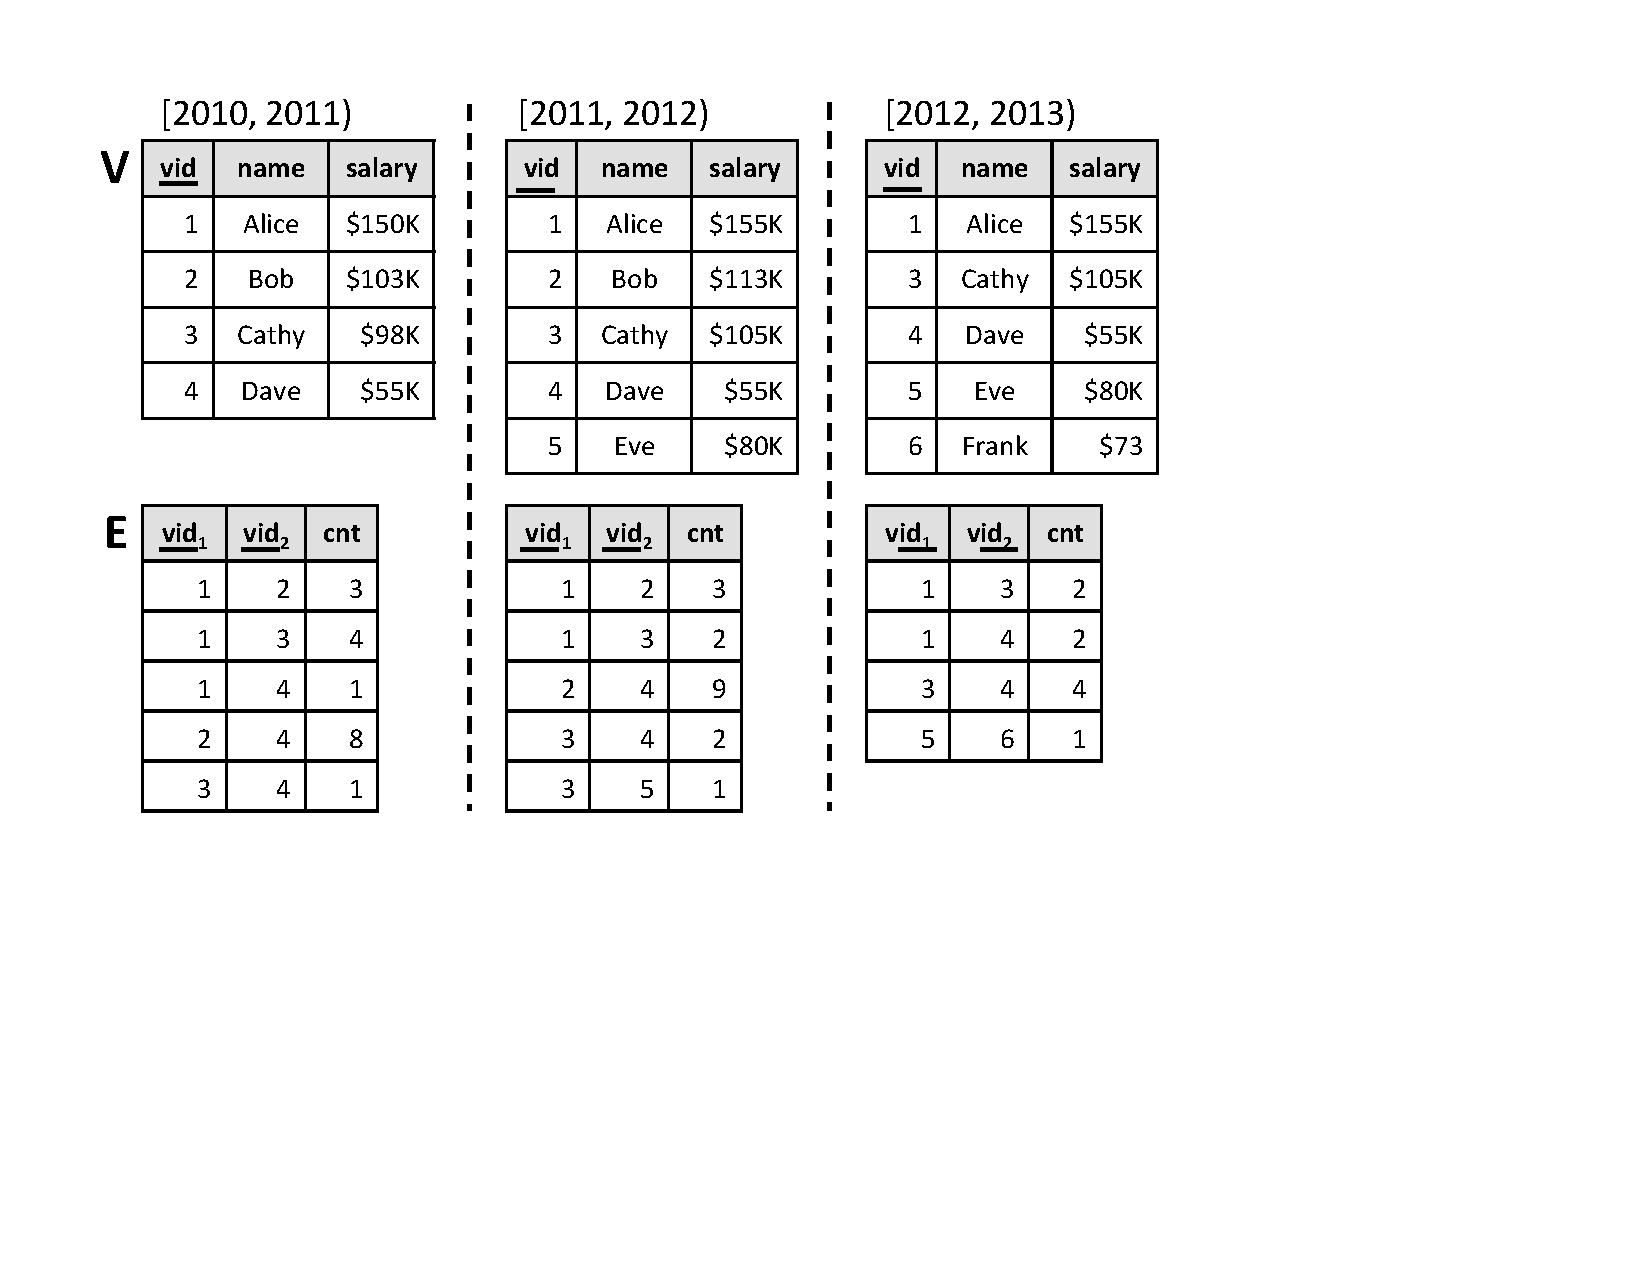
\includegraphics[width=3.5in]{figs/3VE.pdf}
\caption{Vertices and edges of 3 snapshots of \insql{T1}.}
\label{fig:3ve}
\end{figure}

\begin{small}
\begin{verbatim}
Q1: TSelect  V; E
    From     T1
    TWhere   Start >= 2010 And End < 2014
\end{verbatim}
\end{small}

$Q1$ performs temporal selection --- its result is a \tg that contains
a consecutive subset of the snapshots of \insql{T1} that fall within
the interval specified by the \insql{TWhere} clause, namely, $[2010,
  2011)$ through $[2013, 2014)$.  The result of $Q1$ has the same
    structural schema as \insql{T1}. The \insql{Start} or the
    \insql{End} portions of the \insql{TWhere} clause may be omitted.

More generally, the \insql{TWhere} clause supports a variety of
predicates based on which it is determined, for each snapshot in a
\tg, whether that snapshot is to be retained or discarded.  For
example, \insql{TWhere month(Start) like '\%r\%'} will retain all
snapshots that start during a month in which it is safe to eat oysters
(these are months with the letter 'r' in their name), while
\insql{TWhere year(End) \% 4 = 0} will retain snapshots that end in a
leap year, and discard all others.  However, recall from
Definition~\ref{def:tseq} that a temporal sequence, which constitutes
the temporal schema of a \tg, cannot have any gaps.  We enforce this
by never discarding a time interval in the middle of a sequence, but
rather replacing its snapshot with an empty graph $G(V=\emptyset;
E=\emptyset)$.

{\bf Specifying structural schema of the result.  Snapshot analytics.}
Next, consider query $Q2$ below.

\begin{small}
\begin{verbatim}
Q2: TSelect  V [vid, pagerank() as pr]; 
             E [vid1, vid2, cnt * 0.001 as score]
    From     T1
\end{verbatim}
\end{small}

This query illustrates how the \insql{TSelect} clause can be used to
specify the structural schema of the result, which in this case is
V(\underline{vid}:int, pr:float); E(\underline{vid1}:int,
\underline{vid2}:int, score:float).  We may use the \insql{TSelect}
clause to project out non-key columns of \insql{V} and \insql{E}, or
to add columns with computed values.  Data types of computed
attributes \insql{pr} and \insql{score} are determined by the return
type of the expressions that compute them.  Note that key columns of
\insql{V} and \insql{E} must be present in the result.

The value of the attribute \insql{pr} in $Q2$ is computed using a
snapshot analytic function \insql{pagerank()}.  \ql supports a variety
of snapshot analytics --- functions whose values are computed
w.r.t. each snapshot of a \tg --- including degree, shortest paths,
and connected components.  We provide an API that allows developers to
implement custom analytics that can either be computed locally at a
vertex, like degree, or be expressed in the popular Pregel
API~\cite{DBLP:conf/sigmod/MalewiczABDHLC10}.

\subsection{Temporal Aggregation and Join}
\label{sec:example:groupjoin}

{\bf Temporal aggregation} is illustrated by query $Q3$, which, when
executed with \insql{T1} from Figure~\ref{fig:tg} as input, computes
the \tg in Figure~\ref{fig:q3}.

\begin{small}
\begin{verbatim}
Q3: TSelect   Any V ; Any E 
    From      T1
    TGroup    by 2 years
\end{verbatim}
\end{small}

Temporal aggregation is a two-step operation.  First, temporal schema
of the output is computed according to Definition~\ref{def:tgroup}.
Then structural aggregation of Definition~\ref{def:sgroup} is used
over snapshots in the same temporal group.  Note the use of \insql{Any
  V} and \insql{Any E} in the \insql{TSelect} clause of $Q3$,
specifying that $\gamma^{V}$ and $\gamma^{E}$ operate over unions of
vertices and edges.  For an example consider snapshot $[2010, 2012)$
  in Figure~\ref{fig:q3}, which is computed from snapshots $[2010,
    2011)$ and $[2011, 2012)$ of \insql{T1} in Figure~\ref{fig:tg}.

We may use \insql{TGroup by Size} to specify that all snapshots of the
input \tg be aggregated into a 1-snapshot \tg.  This notation will be
useful when we discuss trend analytics later in this section.

\begin{figure}
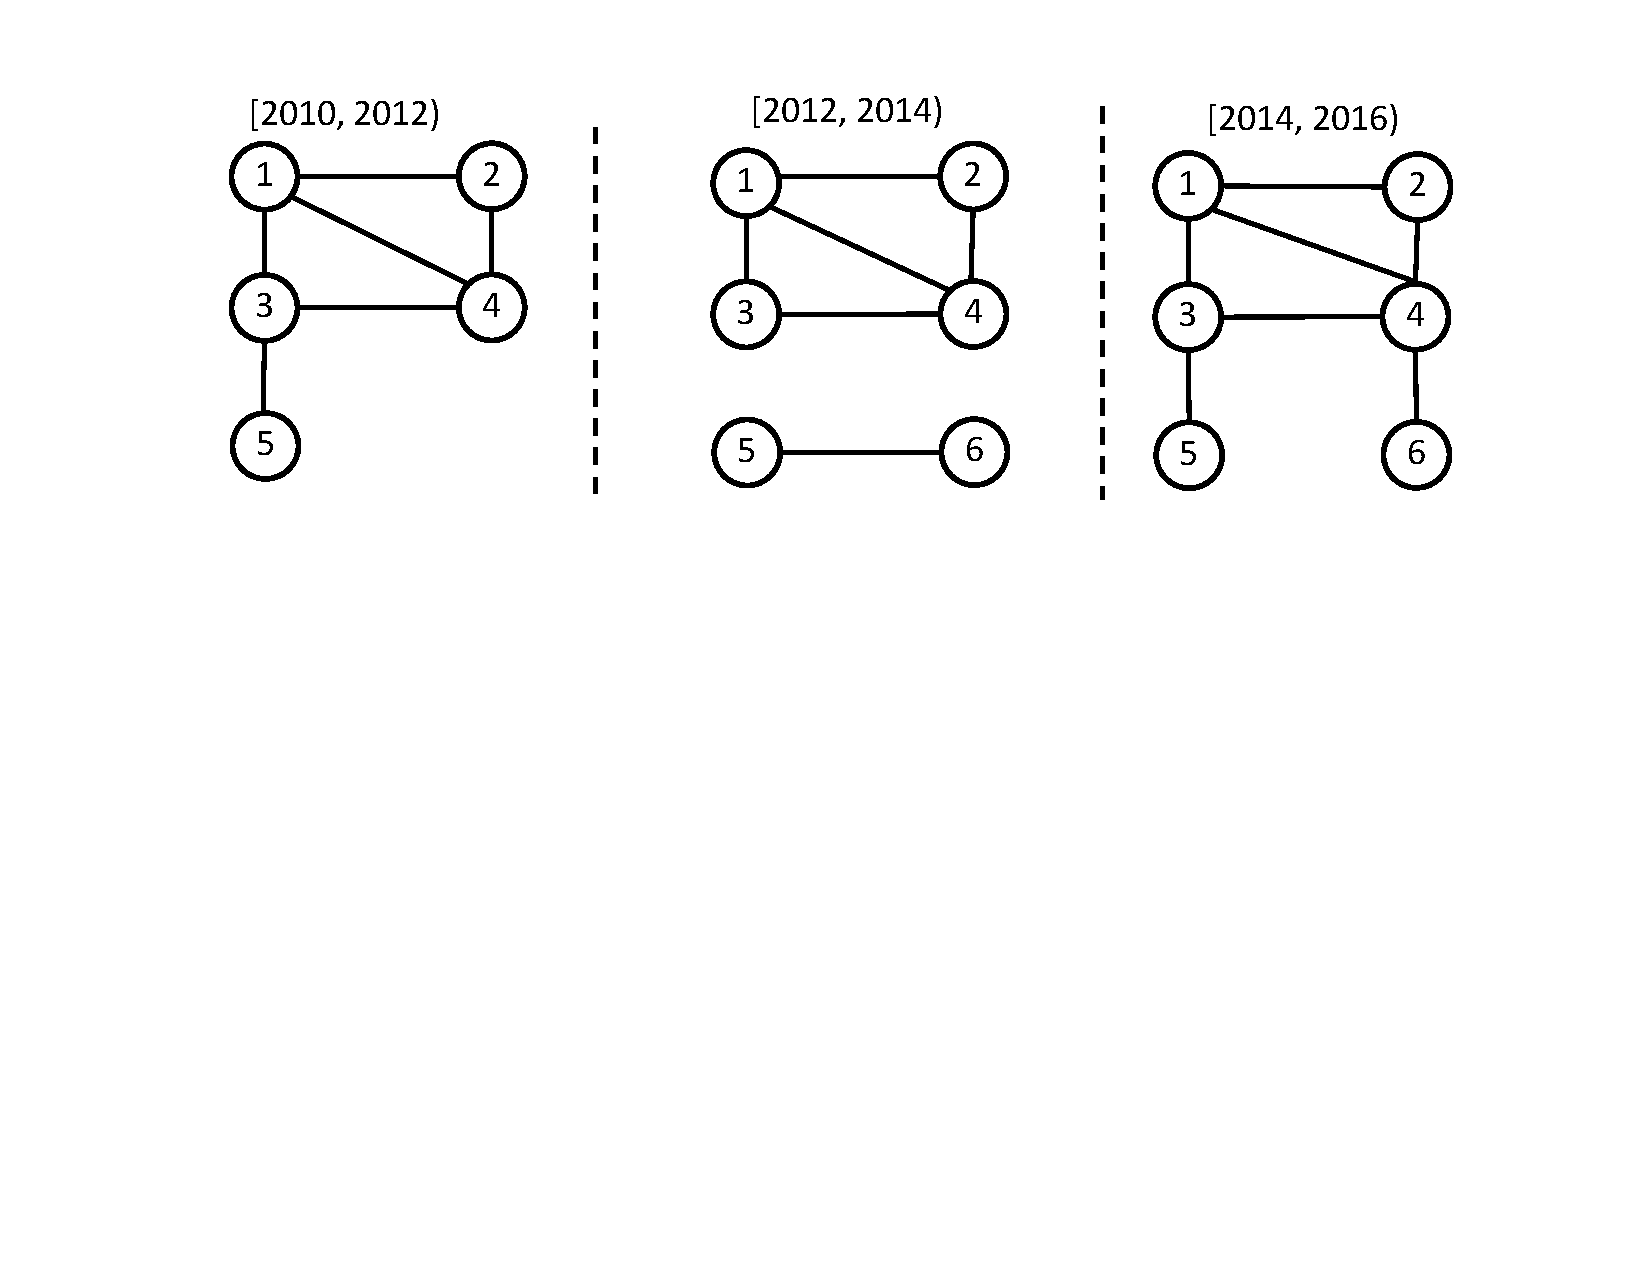
\includegraphics[width=2.5in]{figs/TGroupAny.pdf}
\vspace{-0.1in}
\caption{Result of query Q3 on T1.}
\label{fig:q3}
\end{figure}

Consider next query $Q4$, and its result in
Figure~\ref{fig:tg_all_any}.

\begin{small}
\begin{verbatim}
Q4: TSelect All V [vid, any(name), max(salary)] ; 
            Any E [vid1, vid2, sum(cnt)] 
    From    T1 
    TGroup  by 2 years
\end{verbatim}
\end{small}

The main difference between $Q4$ and $Q3$ is the \insql{All} modifier
associated with vertices in the \insql{TSelect} clause of $Q4$,
meaning that $\gamma^{V}_{vid, any(name), max(salary)}(\bigcap_{G_i
  \in {\cal G}} V(G_i))$ (Definition~\ref{def:sgroup}) is used to
aggregate vertices of snapshots in each 2-year group.  \insql{Any E}
states that the edges in the result correspond to the union of the
edges connecting the vertices.

\begin{figure}
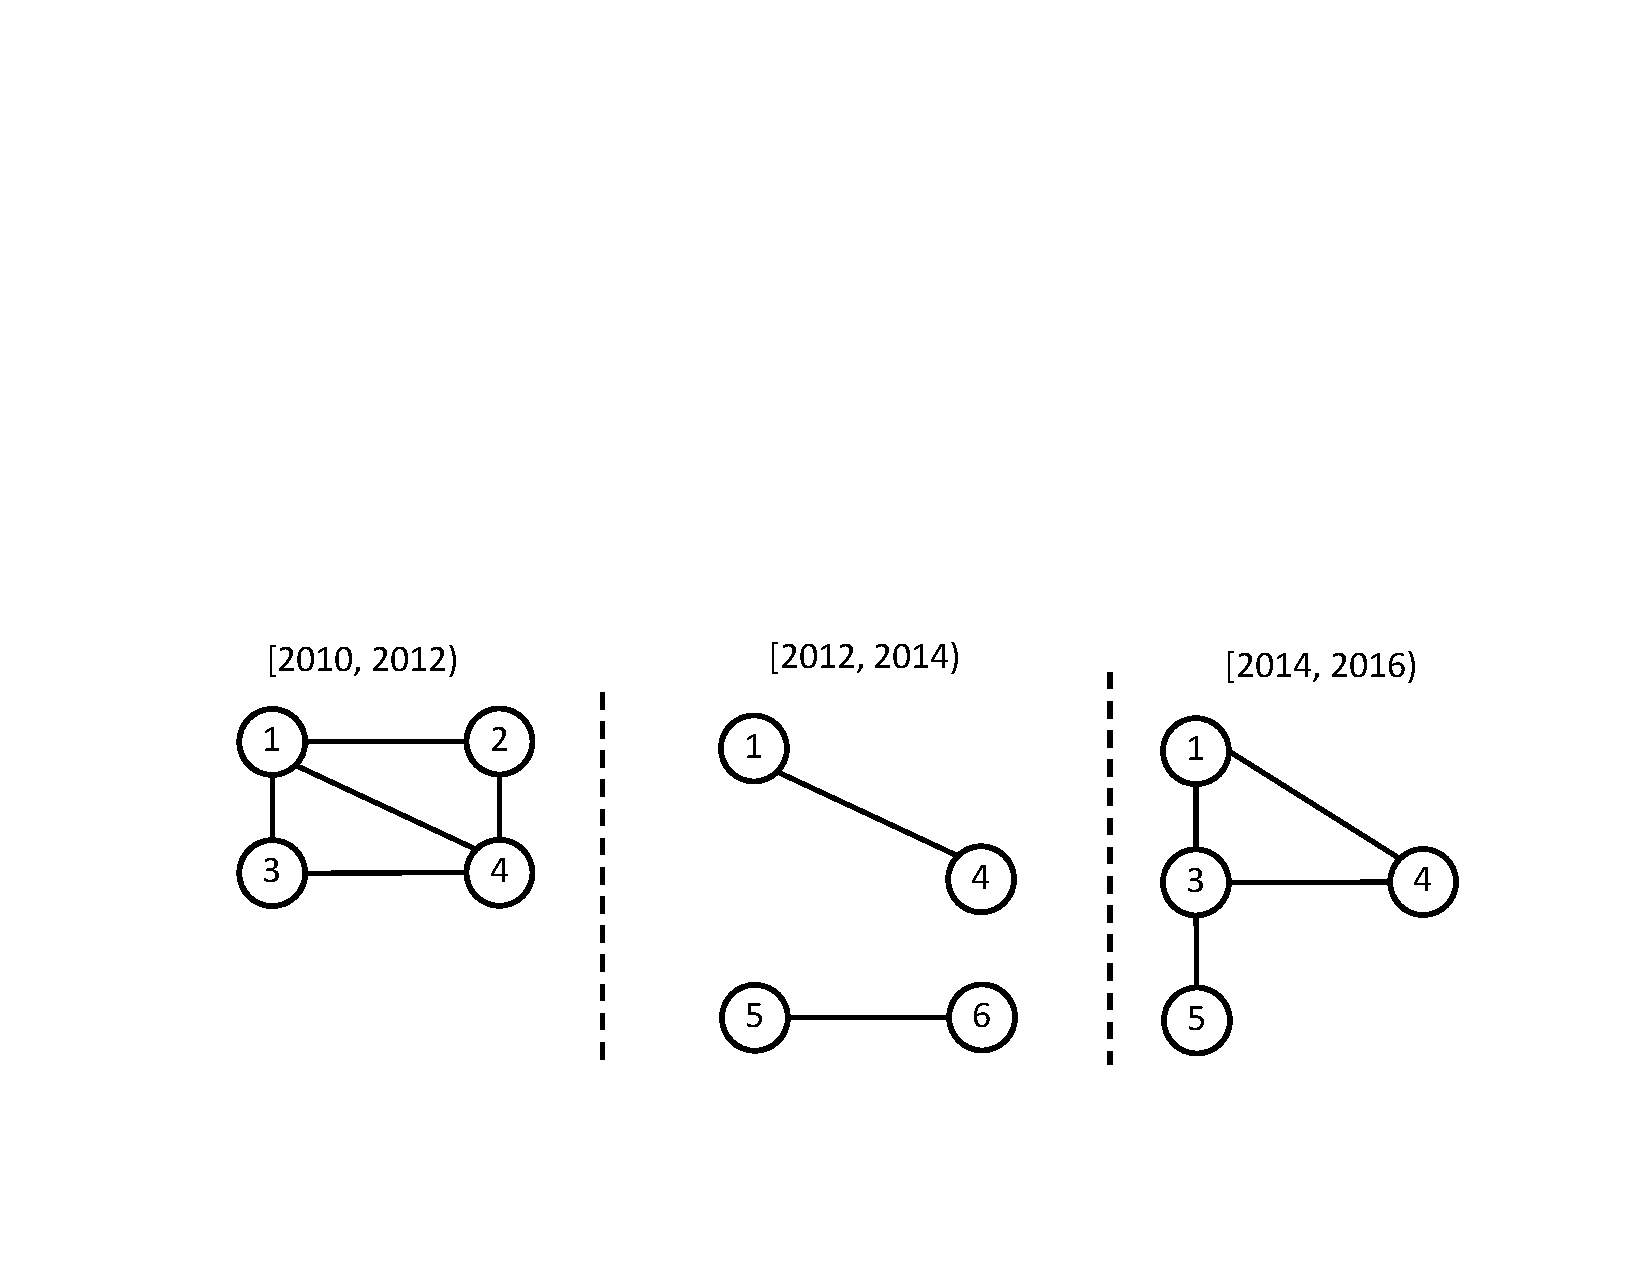
\includegraphics[width=2.5in]{figs/TGroupAllAny.pdf}
\caption{Result of query Q4 on T1.}
\label{fig:tg_all_any}
\vspace{-0.1in}
\end{figure}

$Q4$ illustrates another important feature of \ql, namely, aggregation
of values of non-key attributes of vertices and edges, which takes
place as part of structural aggregation.  We left available operations
unspecified in Definition~\ref{def:sgroup}, so as to keep structural
aggregation generic.  When used in scope of \insql{TGroup}, structural
aggregation operates over an ordered collection of snapshots.  \ql
makes the following aggregation operations available for ordered
snapshot collections: \insql{any}, \insql{first}, \insql{last},
\insql{min}, \insql{max}, \insql{sum}, \insql{count}, and
\insql{list}.

To illustrate, consider vertex and edge relations in
Figure~\ref{fig:3ve}, which correspond to the first three snapshots of
\insql{T1}.  Vertex 1 is present in both $[2010, 2011)$ and $[2011,
    2012)$ in \insql{T1}, and so is present in the snapshot $[2010,
      2012)$ of the result of $Q4$.  Vertex 1 has \insql{name='Alice'}
      in both snapshots, but different values for \insql{salary}.
      Therefore, taking any value of \insql{name} and the maximum
      \insql{salary} may be appropriate.  Operations \insql{first} and
      \insql{last} return the value corresponding to the earliest
      (resp. latest) occurrence of an attribute, while \insql{list}
      returns a collection of all attribute values.

Returning to query $Q3$, when aggregation of attribute values is not
specified explicitly, \insql{any} is used as the default for non-key
attributes.  That is, the \insql{TSelect} clause of $Q3$ is short-hand
for \insql{TSelect Any V[vid, any(name), any(salary)] ;} 
\insql{Any E[vid1, vid2, any(cnt)]}.

{\bf Temporal join.} We will now present two binary operators of \ql
that join together \tg relations, and will illustrate them using
\insql{T1} (Figure~\ref{fig:tg}) and \insql{T2}
(Figure~\ref{fig:tg_t2}).  Query $Q5$ computes temporal intersection
of \insql{T1} and \insql{T2}.  We require that \insql{T1} and
\insql{T2} be union-compatible, as per Definition~\ref{def:tuc}.  The
result of this query is in Figure~\ref{fig:q5}. 

\begin{small}
\begin{verbatim}
Q5:  TSelect   Any V; Any E
     From      T1 TAnd T2
\end{verbatim}
\end{small}

\begin{figure}
\centering
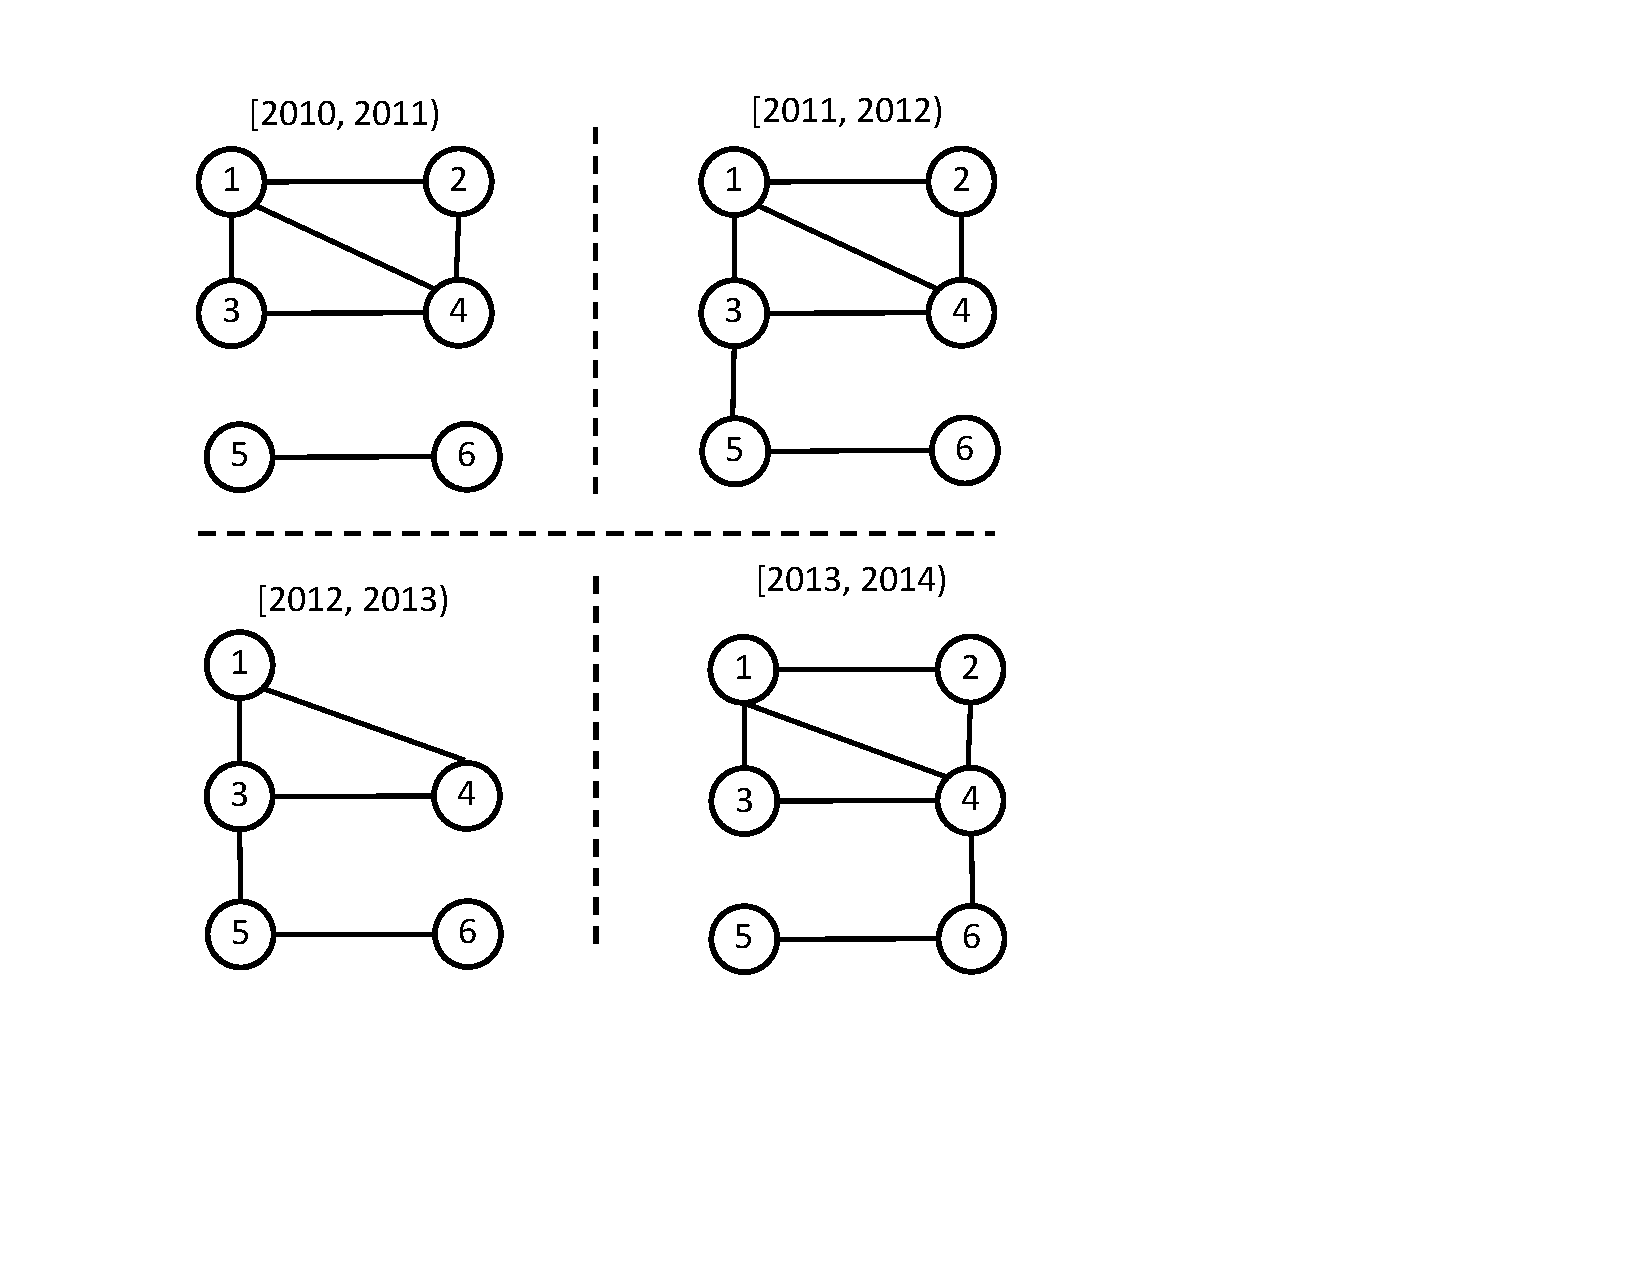
\includegraphics[width=2.8in]{figs/q5.pdf}
\caption{Result of query Q5.}
\vspace{-0.1in}
\label{fig:q5}
\end{figure}

Temporal schema of the result is computed according to
Definition~\ref{def:tseqand}, and corresponds to a sequence with
$P.start = 2010$, $P.end=2014$ and $P.size=4$.  Note the use of
\insql{Any V} and \insql{Any E} in the \insql{TSelect} clause.  This
is another example of structural aggregation
(Definition~\ref{def:sgroup}), now as part of \insql{TAnd}.  The
modifiers \insql{Any} and \insql{All} have the same meaning here as
for \insql{TGroup}, specifying that, a vertex (resp. edge) will be
present in a snapshot in the result if it is present in at least one
corresponding snapshot of \insql{T1} or \insql{T2}.  

An important difference is that, for \insql{TAnd} and \insql{TOr},
structural aggregation operates on unordered collections of snapshots,
with at most two snapshots per group.  \ql makes the following
aggregation operations available for unordered snapshot collections:
\insql{any}, \insql{min}, \insql{max}, \insql{sum}, \insql{count}, and
\insql{list}.  Note that, unlike for \insql{TGroup}, \insql{first} and
\insql{last} are unavailable here, and that \insql{any} is still the
default.

Consider next query $Q6$ that computes temporal union of \insql{T1}
and \insql{T2}.  The result of this query is shown in
Figure~\ref{fig:q6}.

\begin{small}
\begin{verbatim}
Q6:  TSelect   All V[vid, pagerank() as pr]; 
               Any E[vid1, vid2, sum(cnt)]
     From      T1 TOr T2
\end{verbatim}
\end{small}

\begin{figure}
\centering
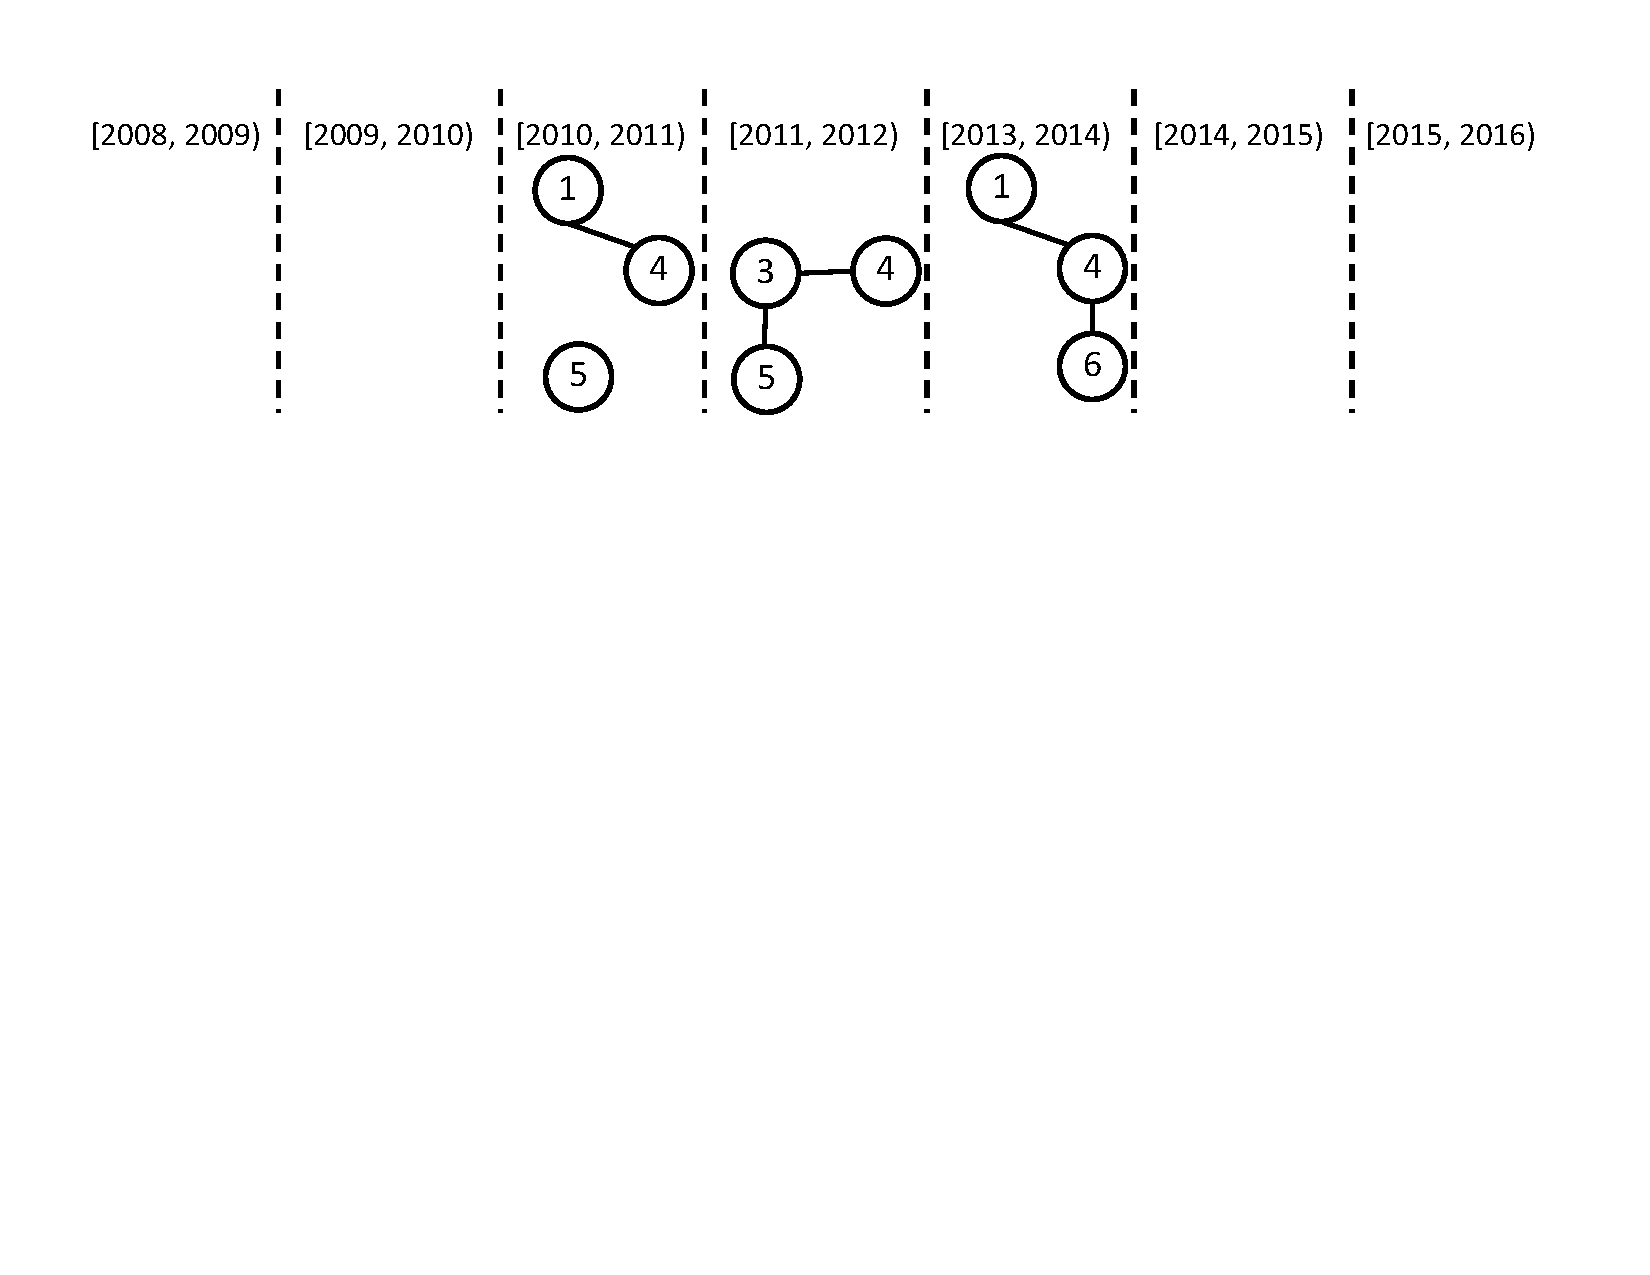
\includegraphics[width=3.4in]{figs/q6.pdf}
\vspace{-0.1in}
\caption{Result of query Q6.}
\label{fig:q6}
\vspace{-0.1in}
\end{figure}

Temporal schema of the result is computed according to
Definition~\ref{def:tseqor}, and corresponds to a sequence with
$P.start = 2008$, $P.end=2016$ and $P.size=8$.  Further, observe the
use of projection (non-key attributes of \insql{V} are not retained),
of an analytic function \insql{pagerank()}, and of the aggregation
operation \insql{sum} applied to the edge attribute \insql{cnt}.

\subsection{Complex queries}
\label{sec:example:complex}

{\bf Order of operators.} So far we illustrated individual operators
of \ql.  Now we will show how multiple operators can be combined in a
single query.  The logical order of evaluation of a \ql query without
nesting is as follows:

\begin{enumerate}
\item Temporal selection in the \insql{TWhere} clause;
\item Temporal join (\insql{TAnd} and \insql{TOr}) in the \insql{From}
  clause;
\item Temporal aggregation in the \insql{TGroup} clause;
\item Projection, computation of attribute aggregates and analytic
  functions.
\end{enumerate}

While the logical order of operations is predetermined, we will see in
Section~\ref{sec:sys:optimization} that some operators can be
reordered without affecting the result (but with potential differences
in performance), while others cannot.  

Consider $Q7$ below, with result shown in Figure~\ref{fig:q7}. $Q7$
first executes temporal selection on each \insql{T1} and \insql{T2}.
(Note that when temporal conditions in the \insql{TWhere} clause are
not qualified, they are applied to all \tgs in the \insql{From}
clause.)  Next, $Q7$ computes temporal intersection of \insql{T1} and
\insql{T2}, and then temporally aggregates the resulting \tg by 2
years.  Finally, \insql{pagerank()} is computed for each vertex in the
result.

\begin{small}
\begin{verbatim}
Q7:  TSelect Any V [vid, pagerank() as pr] ; 
             Any E [vid1, vid2] 
     From    T1 TAnd T2 
     TWhere  Start >= 2012 And End < 2014 
     TGroup  by 2 years
\end{verbatim}
\end{small}

\begin{figure}
\centering
\begin{minipage}{1.6in}
  \centering
  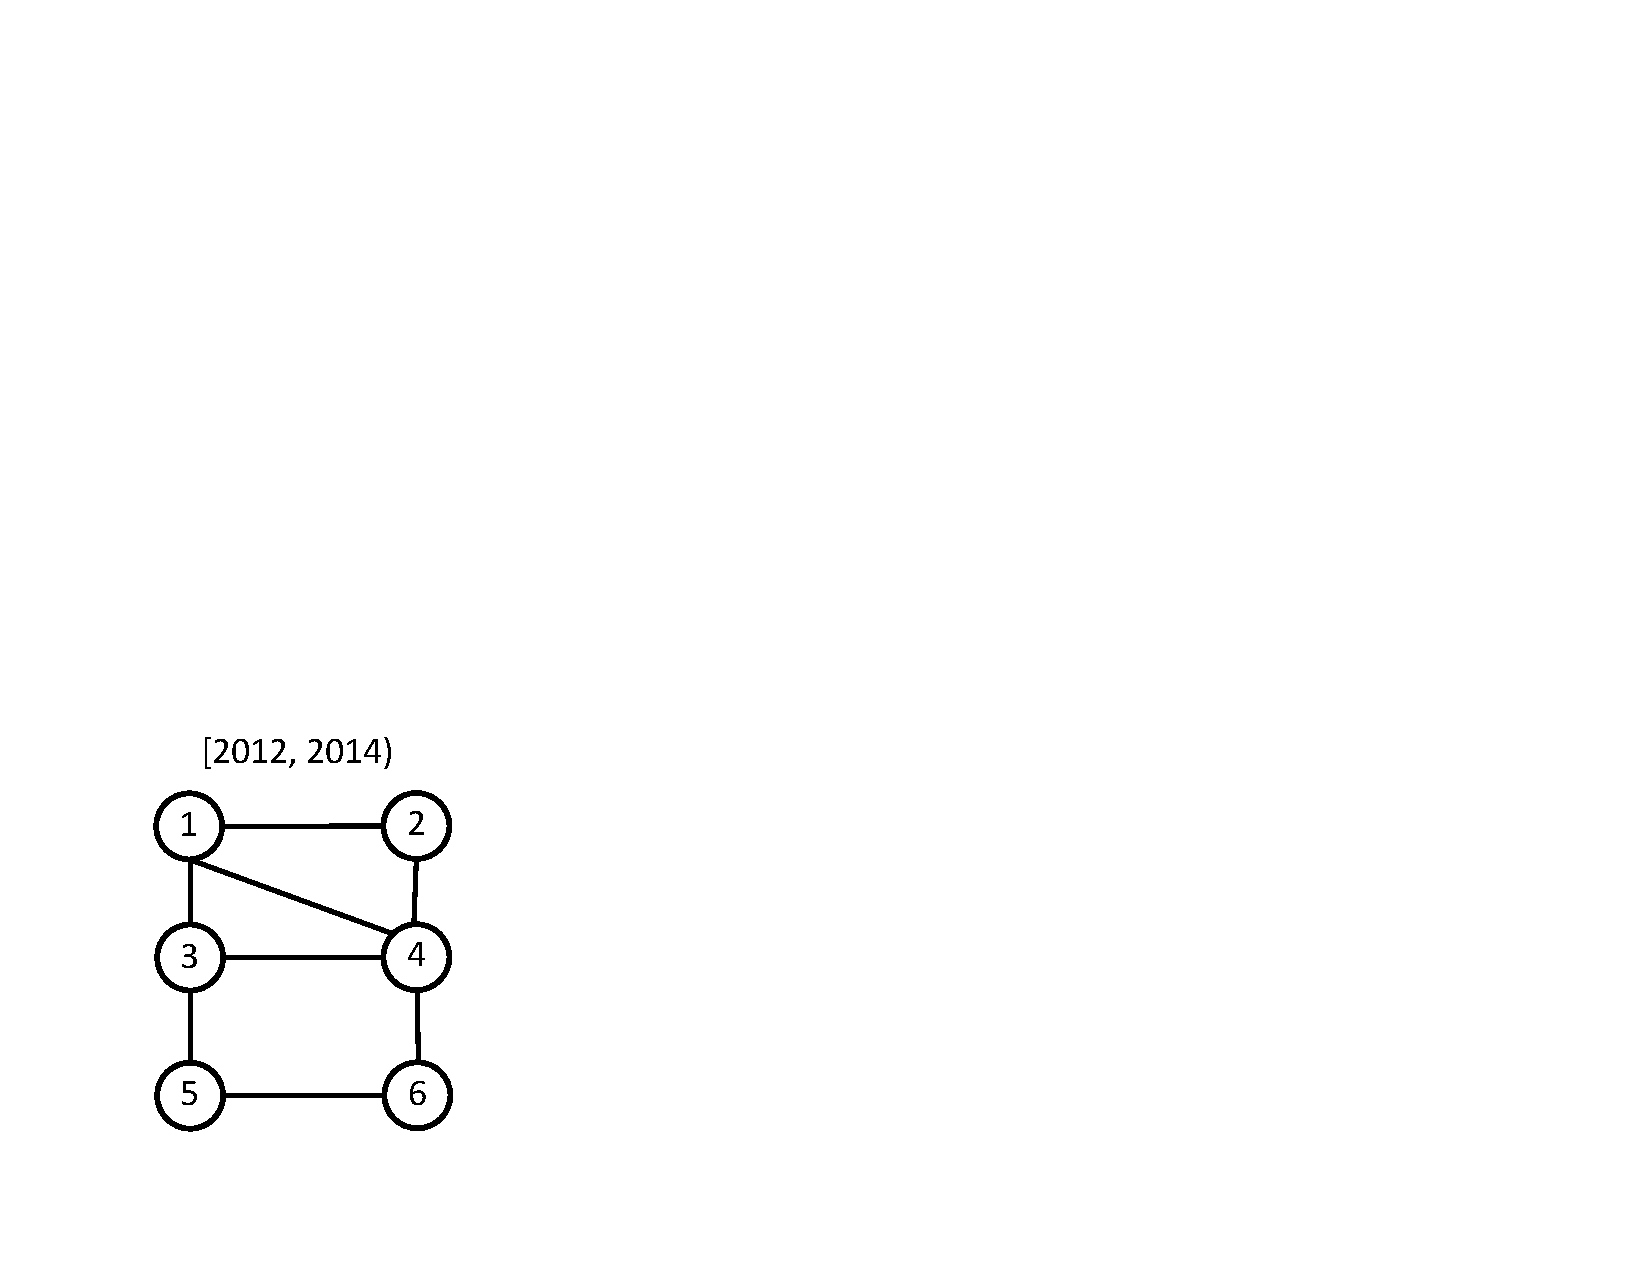
\includegraphics[width=0.8in]{figs/q7.pdf}
\vspace{-0.1in}
  \caption{Result of Q7.}{}
\vspace{-0.1in}
  \label{fig:q7}
\end{minipage}%
\begin{minipage}{1.6in}
  \centering
  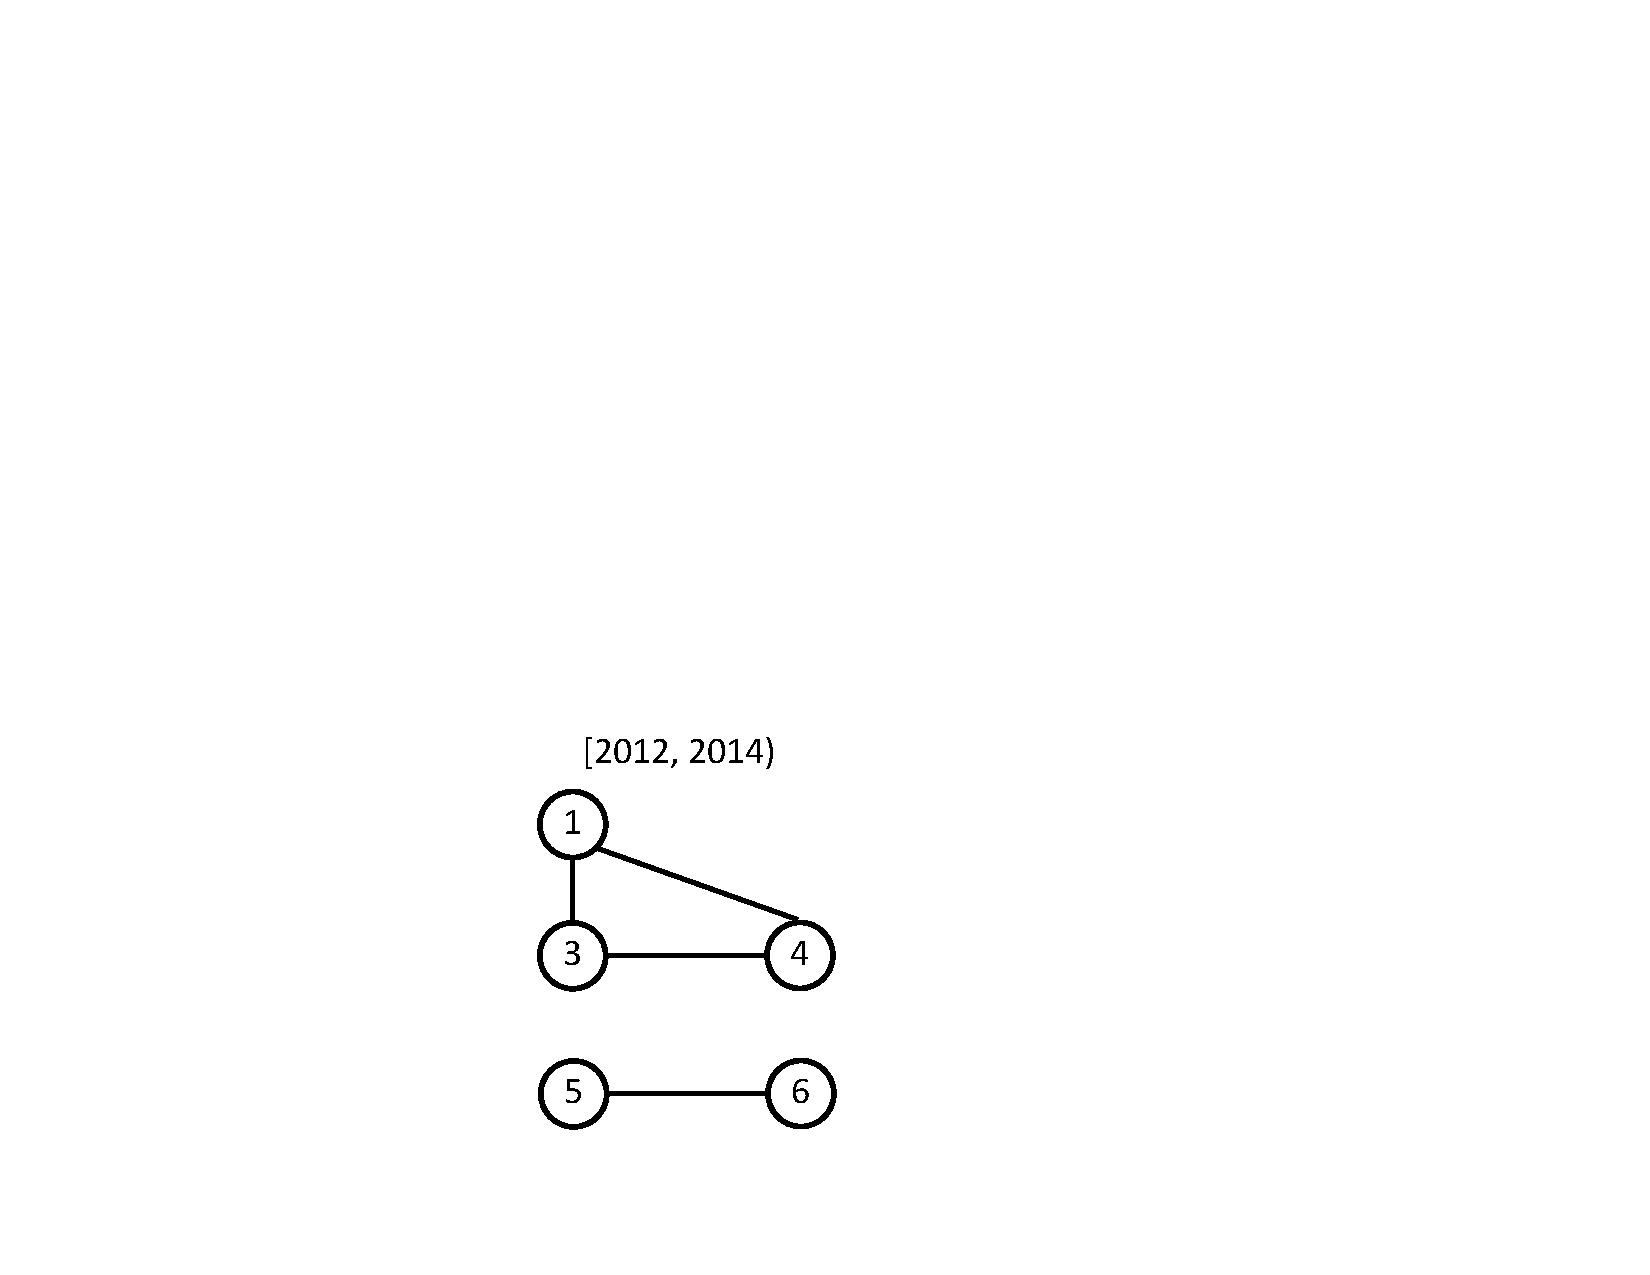
\includegraphics[width=0.8in]{figs/q8.pdf}
\vspace{-0.1in}
  \caption{Result of Q8.}{}
  \label{fig:q8}
\vspace{-0.1in}
\end{minipage}
\end{figure}

Observe that \insql{TAnd} and \insql{TGroup} use the same
specification in the \insql{TSelect} clause, that is, we cannot
decouple structural aggregation behavior of the two operations in a
query of this kind.

Consider next query $Q8$ that is similar to $Q7$, but uses nesting to
decouple structural aggregation of \insql{TSelect} from that of
\insql{TGroup}. The result of executing $Q8$ is shown in
Figure~\ref{fig:q8}.

\begin{small}
\begin{verbatim}
Q8:  TSelect   All V [vid, pagerank() as pr];
               All E [vid1, vid2]
     From      ( TSelect Any V [vid] ; 
                         Any E [vid1, vid2]
                 From    T1 TAnd T2
                 TWhere  Start >= 2012 
                 And     End < 2014 )
     TGroup    by 2 years
\end{verbatim}
\end{small}

{\bf Trend analytics.} We argued in the introduction that it is
important to support analysis of trends in evolving graphs.  The \ql
query language makes this sophisticated analysis possible.  Query $Q9$
illustrates this; it invokes the snapshot analytic \insql{pagerank()}
on \insql{T1}, and then computes the trend in these values across all
snapshots.

\begin{small}
\begin{verbatim}
Q9:  TSelect Any V[vid, trend(pr) as tr, max(pr) as mx];
             Any E[vid1, vid2]  
     From    ( TSelect V[vid, pagerank() as pr];   
                       E[vid1, vid2]
               From    T1 )
     TGroup  by Size
\end{verbatim}
\end{small}

Consider the use of the {\em trend analytic} function
\insql{trend(pr)}, which aggregates the sequence of PageRank scores of
each vertex.  In our implementation we use a common definition of
\insql{trend}: compute the slope of the least squares line using
linear regression, making an adjustment when a vertex value is
missing.  While this is the only trend analytic we currently support,
we are working on an API that will allow developers to implement
custom trend analytics, taking attributes of both atomic and complex
type as input, and computing a value of either an atomic or a complex
type.

We invoke \insql{trend(pr)} alongside \insql{max(pr)} in $Q9$, to
highlight the difference between a trend analytic and value
aggregation.  Syntactically, the two look the same, but the difference
is that \insql{max(pr)} does not account for the temporal order of
values being aggregated, while \insql{trend(pr)} does.  Based on this
distinction, it is not meaningful to invoke a trend analytic when
structural aggregation is due solely to temporal join (\insql{TAnd})
or (\insql{TOr}), but only as part of a query that does temporal
aggregation (\insql{TGroup}).

Finally, recall from our discussion of temporal aggregation that
\insql{TGroup by Size} produces a 1-snapshot \tg.  It is convenient,
although not required, to use this feature in a query such as $Q9$,
since a temporal trend may be computed over a window of any size.

\subsection{Loading data and inspecting results}
\label{sec:example:loadshow}

{\bf Loading filesystem data.  Views.}  Queries $Q1$ through $Q9$
refer to \tg variables in the \insql{From} clause.  The value of a \tg
variable is assigned by the \insql{define view} statement.  This value
may be loaded from the file system, as in query $Q10$, or it may
correspond to a view, as in query $Q11$.

\begin{small}
\begin{verbatim}
Q10:  Create TView T1 as 
        (TSelect V[vid:int, name:str, salary:int]; 
                 E[vid1:int, vid2:int, cnt:int]
         From    path/to/directory)
\end{verbatim}
\end{small}

\begin{small}
\begin{verbatim}
Q11:  Create TView T4 as (TSelect V; E
         From    T1
         TWhere  Start >=  2010)
\end{verbatim}
\end{small}

Note that when data is loaded into a \tg variable from the file
system, as in $Q10$, the \insql{TSelect} clause must specify the
structural schema.  When a \tg variable takes on a value computed by a
query, its structural schema is determined by the query result.  In
$Q11$, the structural schema of the view \insql{T4} is the same as
that of \insql{T1}.

{\bf Inspecting results with SQL.}  Suppose that the result of $Q9$ is
assigned to \insql{T5}, with the structural schema
V(\underline{vid}:int, tr:float, mx:float) ; E(\underline{vid1}:int,
\underline{vid2}:int).  The SQL query below shows \insql{vid}
and \insql{tr} values of 20 vertices with the most significantly
increasing \insql{pagerank} trend.

\begin{small}
\begin{verbatim}
Q12:  Select   VF.vid, VF.tr  
      From     T5.toVerticesFlat() as VF
      Order by tr
      Limit    20
\end{verbatim}
\end{small}

The important part of \insql{Q12} is the use of
\insql{T5.toVerticesFlat()} in the \insql{From} clause.  This is a
multi-step operation provided by the \ql framework, which starts by
collecting all vertices in the union of snapshots of \insql{T5} into a
single nested vertex collection, and associating \underline{vid} with
a time-indexed map of vertex attributes.  Next, the nested collection
is flattened into \insql{VF} (\underline{vid}:int,
\underline{start}:date, \underline{end}:date, tr:float, mx:float).
\insql{VF} can be used in SQL queries.  The \ql framework also
provides an operation that returns a flattened collection of edges,
called \insql{toEdgesFlat()}.





\section{Formal \tga properties}
\label{sec:formal}

Several properties of temporal languages have been studied: temporal
groupedness, temporal semi-completeness, and temporal
completeness~\cite{Bohlen1995}.  We show that the \tg model is
temporally ungrouped but strongly equivalent to the canonical
temporally grouped model.  We also show that \tga is is snapshot
reducible with respect to a generalized nontemporal graph query
language described in~\cite{Wood2012}.  Additionally, we show that
\tga is not temporally semi-complete or temporally complete.  We
review each of these points in turn.  Finally, we study the expressive
power of a fragment of \tga.

\subsection{Temporal Groupedness}

Clifford et al. define two basic strategies for adding temporal
information into the relational model: temporally ungrouped (tuple
timestamping or first-normal-form) and temporally grouped (attribute
timestamping or non-first-normal-form)~\cite{Clifford1994}.  Temporal
relations in \tra, based on the TSQL2 model, are temporally
ungrouped~\cite{Bohlen1995}, since each tuple is associated with its
period of validity.  In such a model, a change to one attribute
results in a new tuple.  In a temporally grouped model related facts
are grouped and their attributes are associated with their individual
periods of validity with the use of a function.

Formally:

\begin{definition}[Canonical temporally ungrouped relation model]
[adapted from~\cite{Clifford1994}, pp. 69-70]  Let $U_D =
\{D_1,\ldots,D_{n_d}\}$ be a set of non-empty value domains, and
$\mathbf{D} = \bigcup^{N_d}_{l=1}D_l$ be the set of all values. Let
$\Omega^T = \{t_0,\ldots,t_i,\ldots\}$ be a non-empty, at most countably
infinite, set of times with total order.  Let $U_A =
\{A_1,\ldots,A_n\}$ be a set of nontemporal attributes, and $T$ a
distinguished time attribute not in $U_A$.

A temporally ungrouped (TU) relation schema $R_{TU}$ is a 3-tuple
$R_{TU} = <\mathbf{A},\mathbf{K},\mathbf{DOM}>$, where:

\begin{itemize}[noitemsep,itemindent=\dimexpr\labelwidth+\labelsep\relax,leftmargin=5pt]
\item $\mathbf{A} \cup \{T\} (\mathbf{A} \subseteq U_A)$ is the set of attributes of the schema.
\item $\mathbf{K} \cup \{T\} (\mathbf{K} \subseteq \mathbf{A})$ is the key of the schema, i.e., $\mathbf{K} \cup \{T\} \to \mathbf{A}$.
\item $\mathbf{DOM}: \mathbf{A} \cup \{T\} \to U_D \cup \{\Omega^T\}$ is a function that assigns domains to attributes in $\mathbf{A}$ and $T$ to $\Omega^T$.
\end{itemize}

A TU database schema $DB_{TU}$ is a finite set of TU relation schemas.
A tuple $rt$ on schema $R_{TU}$ is a function that associates a value
for each attribute $A_i \in \mathbf{A}$ in domain $\mathbf{DOM}(A_i)$
and a value in $T$ to $\Omega^T$.  A TU relation is a finite set of TU
tuples satisfying the key constraint.
\end{definition}

\eat{Observe that the temporal relational schema defined in
Section~\ref{sec:model:temporal} is isomorphic to a temporally
ungrouped relation structure, by using intervals instead of time
points.  This is formally shown in~\cite{Bohlen1995}.}

A canonical temporally grouped relation maintains the notion of an
object changing over time.  We do not include the definition here, refer to~\cite{Clifford1994}.

%Formally:
\eat{
\begin{definition}[Canonical temporally grouped relation model]
[adapted from~\cite{Clifford1994}, pp. 70-71] Let $U_D$, $\mathbf{D}$,
$\Omega^T$, and $U_A$ be defined as for the canonical temporally
ungrouped relation structure above.  Any subset of $\mathbf{L}
\subseteq \Omega^T$ is called a {\em lifespan}.
}
\eat{
A temporally grouped (TG) relation schema $R_{TG}$ is a 3-tuple
$R_{TG} = <\mathbf{A},\mathbf{K},\mathbf{DOM}>$, where:
}
\eat{
\begin{itemize}
\item $\mathbf{A} \subseteq U_A$ is the set of attributes of the schema.
\item $\mathbf{K} \subseteq \mathbf{A}$ is the key of the schema, i.e., $\mathbf{K} \to \mathbf{A}$.
\item $\mathbf{DOM}: \mathbf{A} \to U_D \cup \{\Omega^T\}$ is a
  function that assigns to each attribute a value domain and the
  corresponding temporal domain.
\end{itemize}
}
\eat{
A TG database schema $DB_{TG}$ is a finite set of TG relation schemas.
A tuple $rt$ on schema $R_{TG}$ is a function that associates with
each attribute $A_i \in \mathbf{A}$ a temporal function from the tuple
lifespan to the domain assigned to the attribute $\mathbf{DOM}(A_i)$.
A TG relation is a finite set of TG tuples such that no two tuples
agree on all keys at any instant in time.
\end{definition}
}

What makes TU relations ungrouped is that there is no mechanism to
identify the tuples that correspond to the same entity over time,
i.e., there is no unique grouped relation for an ungrouped relation.
Without a grouping mechanism the TU model and the TG model are only
{\em weakly} equivalent~\cite{Clifford1994}.

The \tg model is ungrouped by the virtue of being expressed over an
ungrouped relational model of \tra.  However, the \tg model requires
that each node and edge have an id that serves as a key and persists
over time, or, in Clifford terminology, it uses constant keys for a
group identifier~\cite{Clifford1994}.  With this restriction the \tga
model is strongly equivalent to the canonical temporally grouped model.

The reasons that we chose the ungrouped model are two-fold: a) it is
the de-facto standard in the temporal relational database community
after more than two decades of discussion, and b) it is easier to
express temporal predicates over the ungrouped model.

\subsection{Temporal Completeness}
\label{sec:formal:reducible}

B{\"{o}}hlen, et al. define two kinds of upwards
  compatability with respect to a nontemporal model: temporal
  semi-completeness and temporal completeness~\cite{Bohlen1995}.  To
  define both we need to recollect the notion of snapshot reducibility.

Snapshot reducibility states that for every nontemporal query $q$ in
language $L$, there must exist a corresponding temporal query $q^t$ in
the temporal language $L^t$ that generalizes $q$~\cite{Dignos2012}.
Note that this definition does not pose any restrictions on the syntax
of the temporal query, so it may be expressed quite differently than
the nontemporal one.  It also does not restrict the temporal language
from having other operators with no nontemporal counterparts.

We can show that \tga is snapshot reducible with respect to
  a particular graph query language.

%For a point-based model, it is customary to interrogate two
%properties --- snapshot reducibility (S-reducibility) and extended
%snapshot reducibility (extended S-reducibility).
%
%S-reducibility states that for every query $q$ in $L$, there must
%exist a syntactically similar query $q^t$ in $L^t$ that generalizes
%$q$ \revision{(Def.~\ref{def:reducibility})}.  Specifically, the
%following relationship should hold when $q^t$ is evaluated over a
%temporal database $D^t$ (recall that $\tau$ is the temporal slice
%operator): $q(\tau_c(D^t)) = \tau_c(q^t(D^t))$, for all time points
%$c$.  Extended S-reducibility requires that $L^t$ provide an ability
%to make explicit references to timestamps alongside non-temporal
%predicates.

\begin{theorem}
\label{theo:reduce}
\tga satisfies the snapshot reducibility properties below with respect
to the generalized graph query language based on the survey by
Wood~\cite{Wood2012}.  $\textsf{snap}_p$ is an operator over \tgs that
computes a graph snapshot at point $p$.

\begin{enumerate}[itemindent=\dimexpr\labelwidth+\labelsep\relax,leftmargin=5pt]
\item $\forall p \in \Omega^T (\textsf{snap}_p(\vmap{f_v,\ttt}) \Leftrightarrow \textsf{map}_v(f_v,\textsf{snap}_p(\ttt)))$

\item $\forall p \in \Omega^T (\textsf{snap}_p(\emap{f_e,\ttt}) \Leftrightarrow \textsf{map}_e(f_e,\textsf{snap}_p(\ttt)))$

\item $\forall p \in \Omega^T (\textsf{snap}_p(\sub{P}{\ttt}) \Leftrightarrow \textsf{subgraph}(P,\textsf{snap}_p(\ttt)))$

\item $\forall p \in \Omega^T (\textsf{snap}_p(\textsf{agg}^T(P,\ttt)) \Leftrightarrow \textsf{agg}(P,\textsf{snap}_p(\ttt)))$

\item $\forall p \in \Omega^T (\textsf{snap}_p(\textsf{node}^T_a(P,\ttt)) \Leftrightarrow \textsf{node}(P,\textsf{snap}_p(\ttt)))$

%\item $\forall p \in \Omega^T (\textsf{snap}_p(\textsf{edge}^T_{P=f_e(\ttt_1.v,\ttt_2.v),f_{v1}(k_1)=f_{v2}(k2)=\ldots=f_{vn}(k_n)=\textsf{any}}(\ttt_1,\ttt_2)) \Leftrightarrow \textsf{snap}_p(\ttt_1) + \textsf{snap}_p(\ttt_2))$ \\($+$ stands for graph join)

%\item $\forall p \in \Omega^T (\textsf{snap}_p(\sub{P_1}{\textsf{edge}^T_{P_2,f_{v1}(k_1)=\ldots=f_{vn}(k_n)=\textsf{any}}(\ttt_1,\ttt_2)}) \Leftrightarrow \textsf{snap}_p(\ttt_1) \odot_{\sigma1,\sigma2,g} \textsf{snap}_p(\ttt_2))$
\end{enumerate}

The equivalences hold for arbitrary \tgs, except equivalence 6, graph
join, which is defined specifically for disjoint graphs.  The only
restriction in this theorem is that any pattern $P$ and mapping
function $f_v$/$f_e$ do not refer to the time attribute.
\end{theorem}

The proof is included in Appendix B.

As noted, snapshot reducibility places no restrictions on the syntax
of the temporal language.  To deal with the syntax, B{\"{o}}hlen, et
al., define a more restrictive type of upward compatability termed {\em
  temporal semi-completeness}~\cite{Bohlen1995} or
S-reducibility~\cite{Bohlen2000}.

\begin{definition}[Temporal semi-completeness]
[\cite{Bohlen1995}, p. 162] Let $M = (DS,L)$ be a nontemporal data
model and $M^T = (DS^t,L^t)$ be a valid-time temporal data model.
Then data model $M^t$ is temporally semi-complete with respect to $M$
iff:

\begin{itemize}[noitemsep,itemindent=\dimexpr\labelwidth+\labelsep\relax,leftmargin=5pt]
\item For every relation $\mathbf{r}$ in $DS$ there exists a temporal
  relation $\mathbf{r^t}$ in $DS^T$ such that $\mathbf{r} =
  \tau_t(\mathbf{r^t})$.
\item For every query $q$ in $L$, there exists a query $q^t$ in $L^t$
  that is snapshot reducible with respect to $q$.
\item There exist two text strings $S_1$ and $S_2$ such that for all
  pairs of queries $(q,q^t)$, where $q^t$ is snapshot reducible to
  $q$, query $q^t$ is syntactically identical to $S_1qS_2$.
\end{itemize}
\end{definition}

The intent of temporal semi-completeness is to provide a kind of
upward compatability that simplifies the transition of nontemporal
language users to the temporal variant.  \eat{For example, TSQL2 provides a
\insql{VALID} keyword that indicates that the query is over the
valid-time temporal semantics.  Interestingly, it has been shown that
TSQL2 is not temporally semi-complete with respect to SQL-92 because
of a) its restriction to duplicate free set semantics, and b) lack of
snapshot reducible counterparts for nested queries~\cite{Bohlen1995}.}

The \tg model meets condition 1, since every snapshot graph
  can be modeled as a \tg with a unit interval as its timestamp.  The
  use of duplicate free set-based semantics is not an issue because
  graph snapshots do not allow duplicates either -- every node and
  edge has an identity.  Condition 2 is also satisfied, as we already
  showed that for every graph operator there is a corresponding \tga
  operator that is snapshot-reducible.

Since \tga does not specify a syntax, requirement 3 cannot
  be satisfied.  The definitions in Section~\ref{sec:algebra} specify
  the semantics of each operator, but do not dictate any specific way
  the operator must be expressed by the user.  For instance, we do not
  specify how the patterns are specified.  Thus \tga cannot be
  considered temporally semi-complete with respect to any graph query
  language.

A further notion of upward compatability is {\em temporal
  completeness}.

\begin{definition}[Temporal completeness]
[\cite{Bohlen1995}, p. 166]  Let $M = (DS,L)$ be a nontemporal data
model and $M^T = (DS^t,L^t)$ be a valid-time temporal data model.
Then data model $M^t$ is temporally complete with respect to $M$
iff:

\begin{itemize}[noitemsep,itemindent=\dimexpr\labelwidth+\labelsep\relax,leftmargin=5pt]
\item $M^t$ is temporally semi-complete with respect to $M$.
\item It is possible to override snapshot reducibility for every
  snapshot reducible query $q^t$ in $L^t$ by some syntactic means such
  as dropping the syntactic extensions that enforce it.
\item Syntactic reducibility can be applied to subqueries.
\item Allen's interval operators or their equivalents can be used in queries.
\item It is possible to refer to both the (a) coalesced interval and (b) original intervals as specified by the user.
\end{itemize}
\end{definition}

Condition 2 is elsewhere termed {\em
  nonrestrictiveness}~\cite{Bohlen2000} and gives the user full
control over the timestamps as regular values if desired. Condition 5
essentially refers to the change preservation property of sequence
semantics~\cite{Dignos2012}, without which the intervals specified by
the user have no special meaning.  Any point semantics coalesces
value-equivalent consecutive and overlapping tuples and does not
preserve user-specified intervals.

\tga is not temporally complete both because it is not temporally
semi-complete and because it uses point semantics, thus violating the
final condition.

%\revision{
%\tga is S-reducible because for each operator in \tga, one of the following hold:}

%\revision{\begin{enumerate}[label=\Alph*]
%\item It is rewritten into a sequence of \tra operators, each of which
%  is S-reducible.
%\item It uses temporal navigational graph patterns (TNGPs).  The
%  semantics of the TNGP, when no temporal predicates are present, per
%  Def.~\ref{def:tngp}, is the same as the semantics of the
%  Navigational Graph Patterns (Def~\ref{def:ngp}), i.e., the patterns
%  are semantically applied to each instance of time.
%\end{enumerate}}

%\revision{\tga is extended S-reducible because for each operator in \tga, it
%allows the user to refer to the timestamp of nodes and edges without
%modifying them directly.
%}

\eat{, either it is rewritten into \tra, which is S-reducible w.r.t. relational algebra, or \tga is s-reducible and extended s-reducible because, as we showed in
Section~\ref{sec:algebra}, every \tga operation can be rewritten into
\tra, which is S-reducible and extended S-reducible w.r.t. relational
algebra.  For those operators that are defined using graph patterns,
we can show the following:}

\eat{\begin{enumerate}
\item That an operation with a temporal navigational graph pattern
  (TNGP) is S-reducible when any regular path expressions in the
  pattern are constrained by a temporal predicate \insql{overlaps}
  such that all edges forming a path must coexist.  In this case the
  TNGP is equivalent to a regular navigational pattern in graph
  algebras (Def.~\ref{def:ngp}) and can be semantically applied to
  every point in time.
\item That an operation with a temporal navigational graph pattern is
  extended S-reducible because it allows the user to refer to the
  timestamp of nodes and edges without modifying them, per
  Def.~\ref{def:tngp}.
\end{enumerate}
}

\eat{For those operators that are defined using graph patterns,
e.g., vertex-subgraph (Def.~\ref{def:subv}), we can convert from one
representation to another in polynomial time, as proven in
Theorem~\ref{tgr_tg}.}

\eat{\vera{Not every operator is currently defined through \tra.  However,
  every one that uses patterns can be rewritten to use a conjunctive
  query.}}

\eat{
\julia{Is this a correct statement?} We showed above that \ql algebra
is TRA-\edgec and TRA-\vertexc.  Further, we showed that every
operation on \ql algebra is expressible by a sequence of \tra
queries. Since \tra is known to be S-reducible and extended S-reducible
with respect to relational algebra~\cite{}, then these properties also
hold over the queries that produce vertices and edges in \ql.}

% Make a connection to sequenced semantics - we don't support change
% preservation.

\eat{
\section{Operation equivalences}
\label{sec:equivalences}
}

\subsection{Expressive Power}
\label{sec:epower}

In this section we study expressiveness of the \tg model, which
consists of the \tg data structure (Definition~\ref{def:tg2}) and of
\tga, an algebra for querying the data structure
(Section~\ref{sec:algebra}). We stress that ours is a valid-time data
model that does not provide transaction-time and bi-temporal support.

{\bf Important note:} We restrict our attention to a subset of \tga
operations, excluding recursive queries.  That is, every operation
where Temporal Navigational Graph Patterns (Def.~\ref{def:tngp}) are
applied is restricted to Basic Graph
Patterns~\cite{DBLP:journals/corr/AnglesABHRV16} with temporal
predicates.  A Basic Graph Pattern is equivalent to a regular
conjunctive query without projection~\cite{Abiteboul1995}.  We also
restrict the property values to atomic types for the purposes of this
discussion.

We start by proposing two natural notions of completeness for a
temporal graph query language.

\begin{definition}
  Let $L^t$ be a temporal relational language and $\tve$ --- a
  relational representation of a temporal graph.  An \edgeq $q^t_e$ in
  $L$ takes a graph $\tve (\tv, \te)$ as input, and
  outputs another graph $\tve'$ on the vertices of $\tve$ such that
  the edges of $\tve'$ are defined by $q^t_e$.  A language is
  $L^t$-\edgec if it can express each $q^t_e$ in $L^t$.
  \label{def:edgecomplete}
\end{definition}

Note that the query $q^t_e$ is not restricted to act on \te alone, and
may refer to the other constituent relation of \tve, namely, \tv.

\begin{definition}
  Let $L^t$ be a temporal relational language, and let $\tve$ be a
  relational representation of a temporal graph.  A \vertexq $q^t_v$
  in $L^t$ takes a graph $\tve (\tv, \te)$ as input, and
  outputs another graph $\tve'$ such that the vertices of $\tve'$ are
  defined by $q^t_v$. A language is $L^t$-\vertexc if it can express
  each $q^t_v$ in $L^t$.
\label{def:vertexcomplete}
\end{definition}

We now refer to definitions~\ref{def:edgecomplete}
and~\ref{def:vertexcomplete} and show that \tga is \edgec and
\vertexc, with respect to the valid-time fragment of temporal
relational algebra (\tra).  \tra is an algebra that corresponds to
temporal relational calculus~\cite{DBLP:reference/db/ChomickiT09b}, a
first-order logic that extends relational calculus, supporting
variables and quantifiers over both the data domain and time domain.

\begin{theorem}
\tga is TRA-\edgec.
\label{th:edgecomplete}
\end{theorem}

\begin{proof}
%  \mathsf{(sketch)}
  The result of every conjunctive edge-query over the vertices of \ttt
  can be expressed by $\sigma_{c} (\tv \times^T \tv)$.  Queries of
  this kind can be expressed by the edge creation operator of \tga
  (Def.~\ref{def:edgecr}), invoked as:\\
  $\insql{edge}^T(q=\sigma_{c} (\ttt_1.\tv \times^T \ttt_2.\tv),\ttt_1
  = \ttt,\ttt_2=\ttt)$\end{proof}

\begin{theorem}
\tga is TRA-\vertexc.
\label{th:vertexcomplete}
\end{theorem}

\begin{proof}
%  \mathsf{(sketch)}
  Every \tra vertex-query can be expressed in \tga
  by a sequence of vertex-subgraph $q^T_v(\tve)$
  (Def.~\ref{def:subv}) and attribute-based node creation
  $\insql{node}^T_a$ (Def.~\ref{def:nodecra}).
  Attribute-based node creation supports Skolem functions, and is
  necessary to handle queries that introduce vertex identifiers.  
\end{proof}



\section{\ql by example}
\label{sec:cases}

We now illustrate the salient features of \ql with examples.  For each
example, we give a declarative query, and a corresponding \tga
expression.  For readability, we start by presenting single-operator
queries, and then combine them into a complex query.

All queries presented here will be available to \sys users during the
demonstration, as described in Section~\ref{sec:demo}.  We do not list
performance results here due to space constraints, and point an
interested reader to~\cite{PortalarXiv2016}, where system performance
is evaluated thoroughly.  We note that all queries described here, and
many others, execute in interactive time.

All queries in this section analyze one typical kind of an evolving
graph, namely, an interaction network, which represents people as
vertices, and interactions between them such as messages,
conversations and endorsements, as edges.  Information describing
people and their interactions is represented by vertex and edge
attributes, respectively.  An example of a publicly available
interaction network is the wiki-talk dataset
(\url{http://dx.doi.org/10.5281/zenodo.49561}), containing messaging
events among Wikipedia contributors over a 13-year period.
Information available about the users includes their username, group
membership, and the number of Wikipedia edits they made.  Messaging
events occur when users post on each other's talk pages.

%Communities over time.
Interaction networks are sparse because edges are short-lived.  As
part of exploratory analysis, we can consider the network at different
temporal resolutions, run a community detection algorithm, e.g.,
compute the connected components of the network, and then consider the
number of connected components and their sizes.  

\eat{To see whether communities form and at what time scale, we can vary
the time scale and compute communities, e.g. through connected
components detection, group the vertices by the community they form
and calculate their size.  We can filter out vertices that represent
communities below a reasonable threshold, for example of size smaller
than two.}

\eat{This example demonstrates a need to compute graph-wide analytics
  such as connected components for each point in time, create new
  vertices that represent some aspect of data of existing vertices,
  and compute subgraphs.  Graph-wide analytics on evolving graphs have
  been proposed previously in ImmortalGraph~\cite{Miao2015} and
  G*~\cite{Labouseur2015}, including PageRank, weakly connected
  components, and source-source shortest path.}

\eat{{\bf Question:} In a sparse communication network, on what time scale
can we detect communities?}

\begin{example}
\label{ex:load}

We can load the dataset with the following command:

\begin{small} 
\begin{verbatim}
Create TGraph wiki As { Load From "path/to/data" }
\end{verbatim}
\end{small}

\end{example}

We use the Apache Parquet format for on-disk storage, with one archive
for vertices and another for edges, temporally coalesced.  We provide
a loader utility that can initialize any of our available physical
representations (see~\cite{PortalarXiv2016}), from Apache Parquet
files on HDFS or on local disk.

\begin{example}
\label{ex:slice}

Select a 5-year subset of the data:

\begin{small} 
\begin{verbatim}
Create TGView T1 As { 
   VSelect * ESelect *
   From wiki
   VWhere start>='2010-01-01' AND end<'2015-01-01'}
\end{verbatim}
\end{small}

\eat{\vera{We have a semantic ambiguity here that we need to fix. Now that
  selection operator accepts temporal predicates, the above can be
  interpreted as either a slice or a selection, with different
  results.}}

The corresponding algebraic expression in \tra uses the common
temporal slice operator: $\ttt_1 = \slice{[2010,2015)}{wiki}$.

\end{example}

\begin{example}
\label{ex:nodecrt}

Compute a temporally aggregated view of the graph into 6-months
windows.  A window includes vertices and edges that correspond to
users who communicated regularly: a vertex and an edge are each
present if they exist in every snapshot during the 6-month period.

\begin{small} 
\begin{verbatim}
Create TGView T2 As { 
   VSelect * ESelect *
   From T1
   TGroup By 6 months
   VExists always EExists always }
\end{verbatim}
\end{small}

This query corresponds to a \tra expression that invokes window-based
node creation, an evolving graph operation similar to moving window
temporal aggregation for relations:
$\ttt_2 = \insql{node}^T_w(\mathsf{w=6~mon},\mathsf{q_v=always},\mathsf{q_e=always},\ttt_1)$.

\end{example}

Node creation enables the user to analyze an evolving graph at
different levels of granularity.  This operator comes in two variants
--- based on temporal window (Example~\ref{ex:nodecrt}) or based
on vertex attributes, illustrated next.

\begin{example}
\label{ex:cc}

Compute connected components at each time point.  This is an
  example of a Pregel-style analytic invocation over an evolving
  graph.

\begin{small} 
\begin{verbatim}
Create TGView T3 As { 
   VSelect components() as comp, *
   Eselect *
   From T2 }
\end{verbatim}
\end{small}

This query correspond to the following \tra expression:
$\ttt_3 = \insql{pregel}^T_{cc} (\mathsf{pname=comp}, \ttt_2)$.

\end{example}

\eat{
Note the use of $*$ after invocation of the components analytic.  With
the property model, different nodes may have different properties, so
listing them all may be burdensome for the user.}

\eat{ We need to compute graph-wide analytics such as connected
  components for each point in time.  Graph-wide analytics on evolving
  graphs have been proposed previously in
  ImmortalGraph~\cite{Miao2015} and G*~\cite{Labouseur2015}, including
  PageRank, weakly connected components, and source-source shortest
  path.}

\begin{example}
\label{ex:nodecra}

Generate a new graph, in which a vertex corresponds to a connected
component, and compute the size of the connected component.  

\begin{small} 
\begin{verbatim}
Create TGView T4 As { 
   VSelect count(*) as cnt  ESelect *
   From T3
   VGroup By comp }
\end{verbatim}
\end{small}

\end{example}

This operation allows the user to generate a \tg in which a vertex
corresponds to a group of vertices in the input that agree on the
values of all grouping attributes.  An edge in the output is
introduced between vertices $g_1$ and $g_2$ if some pair of vertices
$v_1$ and $v_2$ in the input \tg were connected by an edge, $v_1$ is
in group $g_1$ and $v_2$ is in group $g_2$.  We do not add any
self-loops to the output \tg. The corresponding \tra expression is
$\ttt_4 = \insql{node}^T_a(\mathsf{g=comp,f_v=count(1)},\ttt_3)$.

\eat{Vertices of the input are partitioned on their values of the
  grouping attributes.  An edge is created between a pair of vertices
  in the output if some two input Partitioning of the vertices also
  induces a partitioning of the edges.}

\begin{example}
\label{ex:subg}

Filter out vertices that represent communities too small to be of
interest (e.g., of 1-2 people).  

\begin{small} 
\begin{verbatim}
Create TGView T5 As {
   VSelect * ESelect *
   From T4
   VWhere cnt > 2 }
\end{verbatim}
\end{small}

This query corresponds to a \tra expression that invokes the vertex
subgraph operation $\ttt_5 = \subv{\mathsf{v.a.count > 2}}{\ttt_4}$.

\end{example}

The queries of Examples~\ref{ex:load} --- \ref{ex:subg} can be
combined into a single complex query:

\begin{small}
\begin{verbatim}
VSelect * ESelect *
From (
    VSelect count(*) as cnt  ESelect *
    From (
        VSelect components() as comp, * ESelect *
        From ( Load From "path/to/data" }
        TGroup By 6 months
        VExists always EExists always
        VWhere start>='2010-01-01' AND end<'2015-01-01' )
    VGroup By comp)
VWhere cnt > 2 
\end{verbatim}
\end{small}

In an individual \ql query, selection and subgraph operations
(\insql{VWhere} and \insql{EWhere}) take precedence over the other
operations, followed by node creation (\insql{TGroup} and
\insql{VGroup}), and then by aggregation (illustrated in
Example~\ref{ex:agg}) and analytics.  Multiple orders of execution are
possible in queries that include node creation by both temporal window
and vertex attributes, and in queries that join two \tgs by means of
an intersection or a union (illustrated in Example~\ref{ex:union}
below), and execute node creation, selection or subgraph on the
result.  We discuss this further in Section~\ref{sec:sys}.

\eat{The order of precedence in a single statement is selection and
  slice (\insql{vwhere}, \insql{ewhere}), node creation, analytics,
  map, and then binary operations.  Multiple orders of execution are
  possible since slice can be performed at any point, but it is most
  efficient to perform slice first to reduce the amount of data for
  further evaluation.}

Another use case demonstrates the remaining operations of \tga.  DBLP
and arXiv datasets contain co-authorship information and can provide
interesting insights into the CS research community at large.  Nodes
represent authors, and edges --- a joint publication between a pair of
authors.

\begin{example}
\label{ex:union}

Assuming that author ids are drawn from the same domain, i.e., are
assigned consistently in DBLP and arXiv, we can combine the two
datasets for a more comprehensive view using temporal graph union:

\begin{small}
\begin{verbatim}
Create TGView T6 As {
   VSelect left(name)  ESelect max(cnt)
   From dblp Union arXiv }
\end{verbatim}
\end{small}

Note that, unlike in relational algebra, \tga union requires aggregate
functions to resolve multiple property values for the same node or
edge.  The \insql{left} function takes the value of the vertex
property \insql{name} from the DBLP dataset (the left operand), if a
vertex exists in both DBLP and arXiv. The corresponding \tga
expression is $\ttt_6 =
dblp~\cap^T~arXiv(f_v=left(name),f_E=max(cnt))$.

\end{example}

\begin{example}
\label{ex:agg}

Finally, we compute an in-degree of each vertex during each time
point.  This is an example of the {\em aggregation} operation, a
common operation on non-temporal graphs, as defined by the taxonomy of
Wood~\cite{Wood2012}.  Aggregation computes a value for each vertex
based on its neighbors.

\begin{small} 
\begin{verbatim}
Create TGView T7 As { 
   VSelect count(*) as deg, * ESelect *
   From T6
   Aggregate Right }
\end{verbatim}
\end{small}

This query corresponds to a \tra expression that uses temporal
aggregation, listed here with default arguments: $\ttt_7 =
\insql{agg}^T(\mathsf{dir=right},\mathsf{f_m=1},\mathsf{f_a=count},\mathsf{pname=deg},\ttt_6)$.

\end{example}

\eat{Besides the examples above, graph queries commonly include retrieving
a specific node (which can be accomplished through a subgraph) and
k-hop neighborhood of a node.  While general transitive closure
requires recursion, which we do not support, k-hop neighborhoods can
be computed using composition operations like the one defined in
SocialScope~\cite{Amer-Yahia2009}.  We provide temporal versions of
subgraph and generalized edge creation.  Additionally, if multiple
sources of the same graph are available, it is useful to combine or
compare them, which dictates the need for temporal set-theoretic
operators.}

\eat{In Section~\ref{sec:algebra} we formally define the operators of our
graph algebra.  In Section~\ref{sec:exp} we return to these three use
cases. 
}


%\section{Properties of \ql}
\label{sec:props}

\subsection{Reducing operators}
\label{sec:props:reduce}

Spark is not a temporal system.  Following the approach of Dignos et
al.~\cite{Dignos2012} we reduce our temporal operators into a sequence
of nontemporal relational operators, maintaining point semantics.  We
need several operators on individual temporal relations in \tve which
we term {\em primitives}: extend, trim, coalesce, normalize, and
constrain, in order to support the operators of \ql algebra.

\eat{Since our model is using point
semantics, we do not support the property of change preservation.  }

The {\em extend} primitive $\epsilon(\mathbf{r})$ extends a relation
with an additional attribute which for each tuple is equivalent to
that tuple's timestamp.  See~\cite{Dignos2012} for the formal
definition.  The extend primitive allows references to the timestamps
in the temporal predicates and join conditions making time information
into data.

The {\em trim} primitive $\mathcal{I}(\mathbf{r},c)$ modifies the
timestamp of each tuple in a relation $\mathbf{r}$ to the result of
its intersection with input period $c$.  Assuming $A$ is a set of
non-temporal attributes of relation {\bf r}, $z \in
\mathcal{I}(\mathbf{r},c) \iff \exists r \in \mathbf{r}(z.A = r.A
\wedge z.p = r.p \cap c)$.

The {\em coalesce} primitive $\mathcal{C}(\mathbf{r})$ merges adjacent
and overlapping time periods.  This operation, which is similar to
duplicate elimination in conventional databases, has been extensively
studied in the
literature~\cite{DBLP:conf/vldb/BohlenSS96,DBLP:journals/sigmod/Zimanyi06}.
Eager coalescing is not desirable since it is expensive and some
operations may produce correct results (up to coalescing) {\em even
  when computing over uncoalesced inputs}.  \eat{This was discussed in
  the context of temporal relational algebra
  in~\cite{DBLP:conf/vldb/BohlenSS96}.}We will revisit this point in
Section~\ref{sec:sys:coal}.

The {\em normalize} primitive, indicated by $\mathcal{N}_B(r;s)$
produces a set of tuples for each tuple in {\bf r} by splitting its
timestamp into non-overlapping periods with respect to another
relation {\bf s} and attributes {\bf B}.  See~\cite{Dignos2012} for
the formal definition.

The {\em constrain} primitive $\mathcal{K}_k(r;s)$ constrains relation
$\mathbf{r}$ with respect to relation $\mathbf{s}$ by key $k$, such as
removing edges from the result that do not have associated nodes, or
trimming the edge validity period to be within the validity periods of
associated nodes.  It is introduced here because Spark does not have a
built-in way to express foreign key constraints.

The implementation of each of these primitives is discussed in
Section~\ref{sec:sys:maint}.

Our reduction rules assume that the four constituent parts of \tve are
extended and are as follows:

\begin{table*}
\small
\begin{tabular}{ | p{1.4cm} p{2.5cm} c L{12.1cm} | }
\hline
\multicolumn{1}{|l}{\bfseries Operator} & & & \multicolumn{1}{c|}{\bfseries Reduction} \\ \hline
\multicolumn{4}{|l|}{trim = $\mathcal{I}$; coalesce = $\mathcal{C}$; normalize = $\mathcal{N}$; constrain = $\mathcal{K}$} \\ \hline
Slice & $\tau_c (\ttt)$ & $=$ & $\forall x \in \{\tv,\te,\tav,\tae \}, x' = \mathcal{I}( \sigma_{p \cap c} (x), c)$ \\
Subgraph & $\sigma_{C_V,C_E} (\ttt)$ & $=$ & $\tv' = \mathcal{C}(\pi_{v,p} (\sigma_{C_{V1}}(\mathcal{N}_v(\tv, \tav)) \bowtie_{v,p} \sigma_{C_{V2}}(\mathcal{N}_v(\tav,\tv)))),$ \newline $\te' = \mathcal{K}_v(\mathcal{C}(\pi_{v_1,v_2,p} (\sigma_{C_{E1}}(\mathcal{N}_{v_1,v_2}(\te,\tae)) \bowtie_{v_1,v_2,p} \sigma_{C_{E2}}(\mathcal{N}_{v_1,v_2}(\tae,\te))), \tv')),$ \newline $\tav' = \mathcal{K}_v(\sigma_{C_{V2}}(\tav), \tv'),$ \newline $\tae' = \mathcal{K}_v(\sigma_{C_{E2}}(\tae), \tv')$ \\
Map & $map_{M_V,M_E}(\ttt)$ & $=$ & $\{ \tv, \te, \mathcal{C}(map_{M_V}(\tav)), \mathcal{C}(map_{M_E}(\tae) \} $ \\
Intersection & $\ttt_1 \cap^T_r \ttt_2$ & $=$ & $\tv' = \mathcal{C}(\mathcal{N}_v(\tv_1, \tv_2) \cap \mathcal{N}_{v}(\tv_2, \tv_1)),$ \newline $\te' = \mathcal{C}(\mathcal{N}_{v1,v2}(\te_1, \te_2) \cap \mathcal{N}_{v1,v2}(\te_2, \te_1)),$ \newline $\tav' = \mathcal{K}_v(\mathcal{C}(map_r(\mathcal{N}_v(\tav_1, \tav_2) \fullouterjoin_{v,p} \mathcal{N}_v(\tav_2, \tav_1))), \tv'),$ \newline $\tae' = \mathcal{K}_v(\mathcal{C}(map_r(\mathcal{N}_{v1,v2}(\tae_1, \tae_2) \fullouterjoin_{v_1,v_2,p} \mathcal{N}_v(\tae_2, \tae_1))), \tv')$ \\
Union & $\ttt_1 \cup^T_r \ttt_2$ & $=$ & $\tv' = \mathcal{C}(\mathcal{N}_v(\tv_1, \tv_2) \cup \mathcal{N}_{v}(\tv_2, \tv_1)),$ \newline $\te' = \mathcal{C}(\mathcal{N}_{v1,v2}(\te_1, \te_2) \cup \mathcal{N}_{v1,v2}(\te_2, \te_1)),$ \newline $\tav' = \mathcal{C}(map_r(\mathcal{N}_v(\tav_1, \tav_2) \fullouterjoin_{v,p} \mathcal{N}_v(\tav_2, \tav_1))),$ \newline $\tae' = \mathcal{C}(map_r(\mathcal{N}_{v1,v2}(\tae_1, \tae_2) \fullouterjoin_{v_1,v_2,p} \mathcal{N}_v(\tae_2, \tae_1))) \}$ \\
Difference & $\ttt_1 \setminus^T_r \ttt_2$ & $=$ & $\tv' = \mathcal{C}(\mathcal{N}_v(\tv_1, \tv_2) \setminus \mathcal{N}_{v}(\tv_2, \tv_1)),$ \newline $\te' = \mathcal{C}(\mathcal{N}_{v1,v2}(\te_1, \te_2) \cap \mathcal{N}_{v1,v2}(\te_2, \te_1)),$ \newline $\tav' = \mathcal{K}_v(\mathcal{C}(map_r(\mathcal{N}_v(\tav_1, \tav_2) \fullouterjoin_{v,p} \mathcal{N}_v(\tav_2, \tav_1))), \tv'),$ \newline $\tae' = \mathcal{K}_v(\mathcal{C}(map_r(\mathcal{N}_{v1,v2}(\tae_1, \tae_2) \fullouterjoin_{v_1,v_2,p} \mathcal{N}_v(\tae_2, \tae_1))), \tv')$ \\
Semijoin & $\ttt \ltimes_{C_V} \mathbf{r}$ & $=$ & \\
Aggregation & $\gamma_{C_V,C_E,A_V}(\ttt)$ & $=$ & \\
Node creation & $\vartheta_{W,Q_V,Q_E,A_V,A_E}(\ttt)$ & $=$ & \\
Composition & $\ttt_1 sym \ttt_2$ & $=$ & \\
\hline
\end{tabular}
\end{table*}

\eat{
When computing result of an operator over the \ve representation, we
do not require that each intermediate state of the data structure
correspond to a valid \tg, but rather that the final result, which is
usually derived after several steps, be valid.  To have a useful
algebra, we do not reject a change that would lead to a violation in
integrity.  Instead, we compute a consistent result by applying the
resolve, coalesce, and contrain primitives.
}
\eat{
Algorithm~\ref{alg:op} outlines the evaluation of a unary operation
\opp(\tve), overloading \opp as appropriate when applying the
operation to constituent parts of \tve.  Some of the steps in
Algorithm~\ref{alg:op} may be unnecessary because of the properties of
the particular operation, as we will see in the remainder of this
section.  Furthermore, 
}

%\begin{algorithm}[t]
%\caption{Evaluation of a unary operation \opp on \tve}
%\begin{algorithmic}[1]
%\REQUIRE \tg $\tve (\tv; \te; \tav; \tae)$, operation \insql{op}.\\
%\STATE  $\tv' = \cl (\opp(\tv))$\\
%\STATE  $\te' = \cl (\opp(\te))$\\
%\STATE  $\tav' = \cl (\opp(\tav))$\\
%\STATE  $\tae' = \cl (\opp(\tae))$\\
%\STATE  enforce foreign keys on $\te'$ w.r.t. $\tv'$\\
%\STATE  enforce foreign keys on $\tav'$ w.r.t. $\tv'$\\
%\STATE  enforce foreign keys on $\tae'$ w.r.t. $\te'$\\
%\RETURN new $\tve (\tv';\te';\tav';\tae')$\\
%\end{algorithmic}
%\label{alg:op}
%\end{algorithm}

%\section{Lazy Coalescing}
\subsection{Lazy Coalescing}
\label{sec:sys:coal}

\eat{
\begin{table}
\small
\begin{tabular}{ l | p{4cm} | c }
\hline
\multicolumn{1}{l|}{\bfseries Operation} & \multicolumn{1}{c|}{\bfseries Requires Coalesced Input} & \multicolumn{1}{c}{\bfseries Uncoalesces} \\ \hline
slice & no & no \\ \hline
select & only if predicate incl. interval & no \\ \hline
project & no & yes \\ \hline
aggregate & only if structural group by is used and includes interval & yes \\ \hline
union & no & yes \\ \hline
intersection & no & yes \\ \hline
analytics & no & yes \\
\hline
\end{tabular}
\caption{Coalesce analysis.}
\label{tab:coalesce}
\end{table}
}

All operations and all sequences of operations must output a valid
temporally coalesced \tg.  Several implementations are possible for
the coalesce operation over temporal SQL relations,
see~\cite{DBLP:conf/vldb/BohlenSS96} for details.  We use the
partitioning method, where the relation (e.g., \tv, \te, \trg) is
grouped by key, and tuples are sorted and folded within each group to
produce time periods of maximum length.  This involves shuffling
between partitions, is computationally expensive, and motivates
lazy coalescing.

Correctness of many \tg algebra operations does not depend on whether
their input is coalesced.  Consequently, \ql supports both eager and
lazy coalescing, with lazy being the default for queries that admit
it.  We now present useful coalescing rules.

\eat{ As with duplicate elimination, if the coalesced output is
  expected to be significantly reduced in size, such as after a
  project operation on a high volatility attribute, performing
  coalesce eagerly before a time-consuming operation, especially
  analytics, can be advantageous.}
%

\eat{{\bf Successive coalescing is unnecessary} in \tg algebra just as it
is for (non-graph) temporal
databases~\cite{DBLP:conf/vldb/BohlenSS96}:}
\eat{\begin{equation}
\cl(\cl(\ttt)) \equiv \cl(\ttt)
\label{rul:twice}
\end{equation}}

\eat{It is unnecessary to coalesce an already coalesced \ttt, e.g., if the
data on disk is known to be coalesced:}

\eat{\begin{equation} 
\cl(\ttt) \equiv \ttt~~\text{iff}~\textsf{is\_coalesced}(\ttt)
\label{rul:cond}
\end{equation}}

%The first rule eliminates successive coalescing:

%\begin{equation}
%\cl(\cl(\ttt)) \equiv \cl(\ttt)
%\label{rul:coalr0}
%\end{equation}

{\bf Slice allows lazy coalescing.}  We showed in
Section~\ref{sec:algebra:slice} that slice does not destroy
coalescing.  Further, recall that $\tau_c(\cl(\ttt))$ returns tuples
$(x,p \cap c)$, for which $p \cap c \neq \emptyset$.  If \ttt is
uncoalesced, then there exist some value-equivalent tuples $(x, p_1)$
and $(x, p_2)$
s.t. $\pred{p_1}{meets}{p_2}~\lor~\pred{p_1}{contains}{p_2}~\lor$\\$\pred{p_1}{overlaps}{p_2}$,
which would be replaced by $(x, p_1 \cup p_2)$ in \cl(\ttt).  Because
intersection distributes over union, i.e.,$(p_1 \cup p_2) \cap c =
(p_1 \cap c) \cup (p_2 \cap c)$, coalescing can be equivalently
performed before or after slice: \eat{$\cl(\tau_c(\ttt)) \equiv
\tau_c(\cl(\ttt))$.}
\begin{equation}
\cl(\tau_c(\ttt)) \equiv \tau_c(\cl(\ttt))
\label{rul:slice}
\end{equation}

{\bf Temporal subgraph may allow lazy coalescing.} It was shown
in~\cite{DBLP:conf/vldb/BohlenSS96} that coalescing can be deferred
until after selection if the selection condition is independent of the
valid time of the input. If temporal subgraph
(Section~\ref{sec:algebra:subgraph}) is time-invariant, coalescing can
be deferred.  \eat{Subgraph does not uncoalesce \tve but may
  uncoalesce \trg (Section~\ref{sec:algebra:subgraph}). For this
  reason it is required to coalesce the final output in
  Rule~\ref{rul:subgraphrg} even if the input was eagerly coalesced,
  but this is not required in Rule~\ref{rul:subgraphve}.}
\begin{multline}
\cl(\sigma_{C_V,C_E}(\ttt)) \equiv \sigma_{C_V,C_E}(\cl(\ttt))\\ \text{iff } independent\_of\_p(C_V) \wedge independent\_of\_p(C_E)
\label{rul:subgraphve}
\end{multline}
\eat{\begin{equation}
\cl(\sigma_{C_V,C_E}(\trg)) \equiv \cl(\sigma_{C_V,C_E}(\cl(\trg)))
\label{rul:subgraphrg}
\end{equation}}

Deferring coalescing can be quite effective for Rules~\ref{rul:slice}
and ~\ref{rul:subgraphve} if the selectivity of the predicate is high.

{\bf Temporal map may allow lazy coalescing}, since it processes each
input tuple without modifying the corresponding time intervals, as
long as it is time-invariant.  Map destroys coalescing
(Section~\ref{sec:algebra:project}), and requires to coalesce the
output even if the input was eagerly coalesced.
\begin{multline}
\cl(\map_{M_V,M_E}(\ttt)) \equiv \cl(\map_{M_V,M_E}(\cl(\ttt)))\\ \text{iff } independent\_of\_p(M_v) \wedge independent\_of\_p(M_E)
\label{rul:map}
\end{multline}

\eat{Rules in ~\ref{rul:coalr1,rul:coalr2,rul:coalr3} exploit the fact that
some operations preserve coalescing, as shown in
Section~\ref{sec:algebra}:}

\eat{\begin{equation}
coal(\tau_c(coal(T))) \equiv \tau_c(coal(T))
\label{rul:coalr1}
\end{equation}
\begin{equation}
coal(\sigma_f(coal(\tve))) \equiv \sigma_f(coal(\tve))
\label{rul:coalr2}
\end{equation}
\begin{equation}
coal(udf(coal(T))) \equiv udf(coal(T))
\label{rul:coalr3}
\end{equation}}

\eat{Rules in
~\cref{rul:coalr4,rul:coalr5,rul:coalr6,rul:coalr7,rul:coalr8,rul:coalr9}
cover operations which are invariant with respect to time and so
coalescing can be postponed until after the operation:}

\eat{\begin{equation}
\tau_c(coal(T)) \equiv coal(\tau_c(T))
\label{rul:coalr4}
\end{equation}}

\eat{Recall that slice selects each entity with an interval that intersects
with $c$ and modifies only the selected tuple periods to $p \cap c$.
According to the rule~\ref{rul:coalr1}, slice does not uncoalesce.  If
the input relation is uncoalesced, it contains some value-equivalent
tuples with adjacent or overlapping periods.  According to the
definitions of $intersect$ and $coalesce$, an intersect with interval
$p$ is the same as the coalesce of intersects of intervals composing
$p$.  I.e., $p \cap c = (p1 \cap c) \cup (p2 \cap c$) where $p = p1
\cup p2$.  Thus coalescing can be performed before or after slice.}

\eat{\begin{equation}
coal(\sigma_f(coal(T))) \equiv coal(\sigma_f(T))
\label{rul:coalr5}
\end{equation}}

\eat{As shown in~\cite{DBLP:conf/vldb/BohlenSS96}, coalescing can be
deferred until after the selection if the selection condition is
independent of the valid time of the input. Since subgraph is a
time-invariant form of select, coalesce is not required prior to
subgraph.  For both this rule and the slice rule above, deferring
coalescing can be quite effective if the selectivity of the predicate
is high.}

\eat{\begin{equation}
coal(\mu(coal(T))) \equiv coal(\mu(T))
\label{rul:coalr6}
\end{equation}}

\eat{The map operation processes each tuple without modifying the
corresponding intervals and independently of the valid time of the
input.  Thus, as above, coalesce can be deferred.}

\eat{\begin{equation}
coal(coal(T_1) \cap coal(T_2)) \equiv coal(T_1 \cap T_2)
\label{rul:coalr7}
\end{equation}}

\eat{\begin{equation}
coal(coal(T_1) \cup coal(T_2)) \equiv coal(T_1 \cup T_2)
\label{rul:coalr8}
\end{equation}}

\eat{For \trg, temporal graph intersection is a inner theta-join followed
by projection.  As shown in~\cite{DBLP:conf/vldb/BohlenSS96},
coalescing can be deferred until after a join and after a projection
if that projection is independent of the valid time interval of the
tuple, which is the case here.  Thus we can defer coalescing until
after the temporal graph intersection.  Temporal graph union is also a
join, albeit an outer one, so the same argument applies.}

\eat{\begin{equation}
coal(udf(coal(T))) \equiv coal(udf(T))
\label{rul:coalr9}
\end{equation}}

{\bf Temporal aggregation requires eager coalescing.}  When
aggregating by change, the input must be coalesced to compute correct
aggregation windows.  If the input is not coalesced, then there may be
two or more consecutive intervals which should be treated as one but
would count separately. For aggregation by time, some aggregate
functions also require coalesced input.  For example, \insql{count}
will produce different result if several consecutive or overlapping
value-equivalent tuples fall within the same window.  Thus we add the
following conditional coalescing rule:
\begin{fleqn}[0pt]
\begin{multline}
\cl(\gamma_{W,Q_V,Q_E,A_V,A_E}(\cl(\ttt))) \equiv \cl(\gamma_{W,Q_V,Q_E,A_V,A_E}(\ttt)) \\
\text{iff}~~W \text{by\_time} \wedge A_V, A_E \in \{\insql{any},\insql{first}, \insql{last},\insql{min}, \insql{max} \}
\label{rul:agg}
\end{multline}
\end{fleqn}

\insql{any} returns any one of the values associated with a property
within each group in $W$, and so is invariant to time and to the
number of tuples in $W$.  \insql{first} and \insql{last} pick the
earliest (resp. latest) value within each group in $W$.  If \ttt is
uncoalesced, there is at least one pair of value-equivalent tuples
with overlapping or consecutive periods.  Selecting between equivalent
values will generate the same result.  The same argument applies to
\insql{min} and \insql{max}.

{\bf Temporal intersection and union allow lazy coalescing.} For \trg,
temporal graph intersection (Section~\ref{sec:algebra:join}) is a join
followed by projection.  As shown in~\cite{DBLP:conf/vldb/BohlenSS96},
coalescing can be deferred until after a join, and after a projection
if projection is independent of the valid time interval of the tuple,
which is the case here.  Thus we can defer coalescing until after
temporal graph intersection.  Temporal graph union
(Section~\ref{sec:algebra:outerjoin}) is an outer join, and the same
argument applies.  Note that both operations may destroy coalescing,
and so a final coalesce is required over the result even if inputs
were eagerly coalesced.
\begin{equation}
\cl(\cl(\ttt_1) \cap \cl(\ttt_2)) \equiv \cl(\ttt_1 \cap \ttt_2)
\label{rul:intersect}
\end{equation}
\begin{equation}
\cl(\cl(\ttt_1) \cup \cl(\ttt_2)) \equiv \cl(\ttt_1 \cup \ttt_2)
\label{rul:union}
\end{equation}

{\bf Temporal user-defined analytics allow lazy coalescing.} If \trg
is not coalesced, it contains one or more value-equivalent
representative graphs with consecutive or overlapping periods.
Analytics are time-invariant functions applied to each representative
graph.  Thus when applied to value-equivalent graphs, they will
produce equivalent results, and so coalesce can be deferred.  Further,
analytics to not destroy coalescing, and so it is not required to
coalesce again over the final result.  
\begin{equation}
\cl(\uda(\ttt)) \equiv \uda(\cl(\ttt))
\label{rul:analytic}
\end{equation}
Although it is possible to defer coalesce for analytics, this will not
be done in practice.  Analytics are computationally expensive, and it
is usually beneficial to eagerly coalesce the input, reducing the
number of representative graphs.

%Finally, a rule that eliminates coalescing of coalesced \tgs:

\eat{\begin{equation}
coal(T) \equiv T~~iff~~is\_coalesced(T)
\label{rul:coalr11}
\end{equation}}

%This last rule is very useful if the data on disk is known to be
%coalesced.


\subsection{Expressive power}
\label{sec:props:power}

todo


%\section{System}
\label{sec:sys}

\begin{figure}[t]
\centering
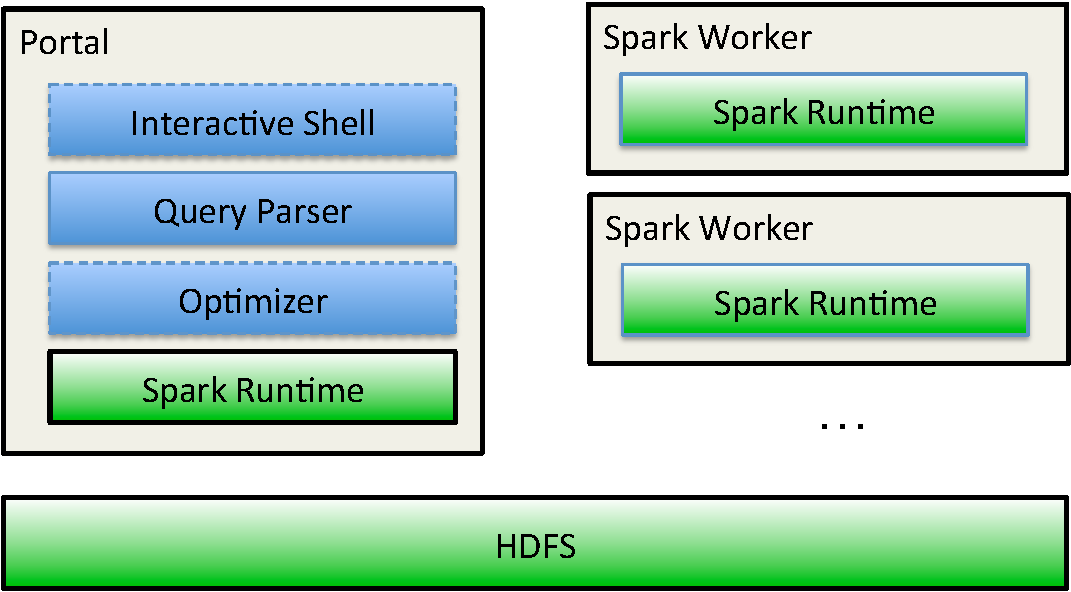
\includegraphics[width=3in]{figs/architecture.pdf}
\vspace{-0.5cm}
\caption{\sys system architecture.}
\vspace{-0.5cm}
\label{fig:arch}
\end{figure}

We developed a prototype system \sys that is implemented on top of
Apache Spark/GraphX~\cite{DBLP:conf/osdi/GonzalezXDCFS14}/Spark
SQL~\cite{Armbrust2015}, as depicted in Figure~\ref{fig:arch}.  Green
boxes indicate built-in components, while blue are those we added for
\sys.  Data is distributed in partitions across the cluster workers,
is read in from the distributed file system (HDFS), and can be viewed
both as a graph and as a pair of RDDs.  All \tg operations are
available through the public API of the \sys library, and may be used
in an Apache Spark application.

{\bf Temporal operators.}  Apache Spark is not a temporal DBMS but
rather an open-source in-memory distributed framework that combines
graph-parallel and data-parallel abstractions.  We reduce our temporal
operators into a sequence of non-temporal relational operators or
their equivalents for Spark RDDs, maintaining point semantics.  While
the TGA is based on relational algebra, multiple transformations are
required for some operations and we use other, more efficient, access
methods where it makes sense.  In some cases, such as temporal window
node creation, access methods based on GraphX graphs provide
significantly more efficient performance.  For analytics, we use the
GraphX Pregel library, but add a batching method to compute overall
time instances together, see~\cite{MoffittTempWeb16} for a detailed
discussion.\eat{ \sys supports PageRank, connected components, and
  shortest paths analytics out of the box, and provides an API for
  adding others.  We are in the process of adding the clustering
  coefficient analytic.}

{\bf Query evaluation.}  \sys query execution follows the traditional
query processing steps: parsing, logical plan generation and
verification, and physical plan generation. \sys re-uses and extends
SparkSQL classes for these steps, including expressions, query tree,
etc, but not the SparkSQL execution engine.  A \ql query is rewritten
into a sequence of \tga operators, and some operators are reordered in
a rule-based manner to improve performance.

Similar to SQL, we apply attribute pruning (column pruning in SQL) and
collapse multiple filters into one.  Slice is always pushed to the
bottom of the tree, except when it appears after temporal window node
creation.  We also add slice to each subtree of the query execution
plan of temporal intersection, based on information about temporal
ranges of \tgs stored in the system catalog.  \eat{E-subgraph is
  pushed through v-subgraph if e-subgraph has no temporal predicate
  because this leads to smaller join size in v-subgraph during
  integrity constraint enforcement.}Unlike selection in SQL, filters
cannot be pushed down through union because of the aggregation
functions.  (See extended discussion on the need for aggregation
functions in set-based operators in~\cite{PortalarXiv2016}).
Attribute-based node creation is always placed before temporal node
creation and temporal union, because it leads to a reduction in
intermediate result size.

We developed several physical representations and partitioning
strategies, selected at the physical plan generation stage.  One
representation mirrors the logical data model and translates \tga
operators into RDD transformations.  Other representations are
graph-based, use the GraphX library, and are more efficient under
certain conditions.  \tgs are read into memory from HDFS and processed
by Spark Workers, with task assignment managed by the runtime.
Details can be found in~\cite{PortalarXiv2016}.

\begin{figure}[t]
\centering
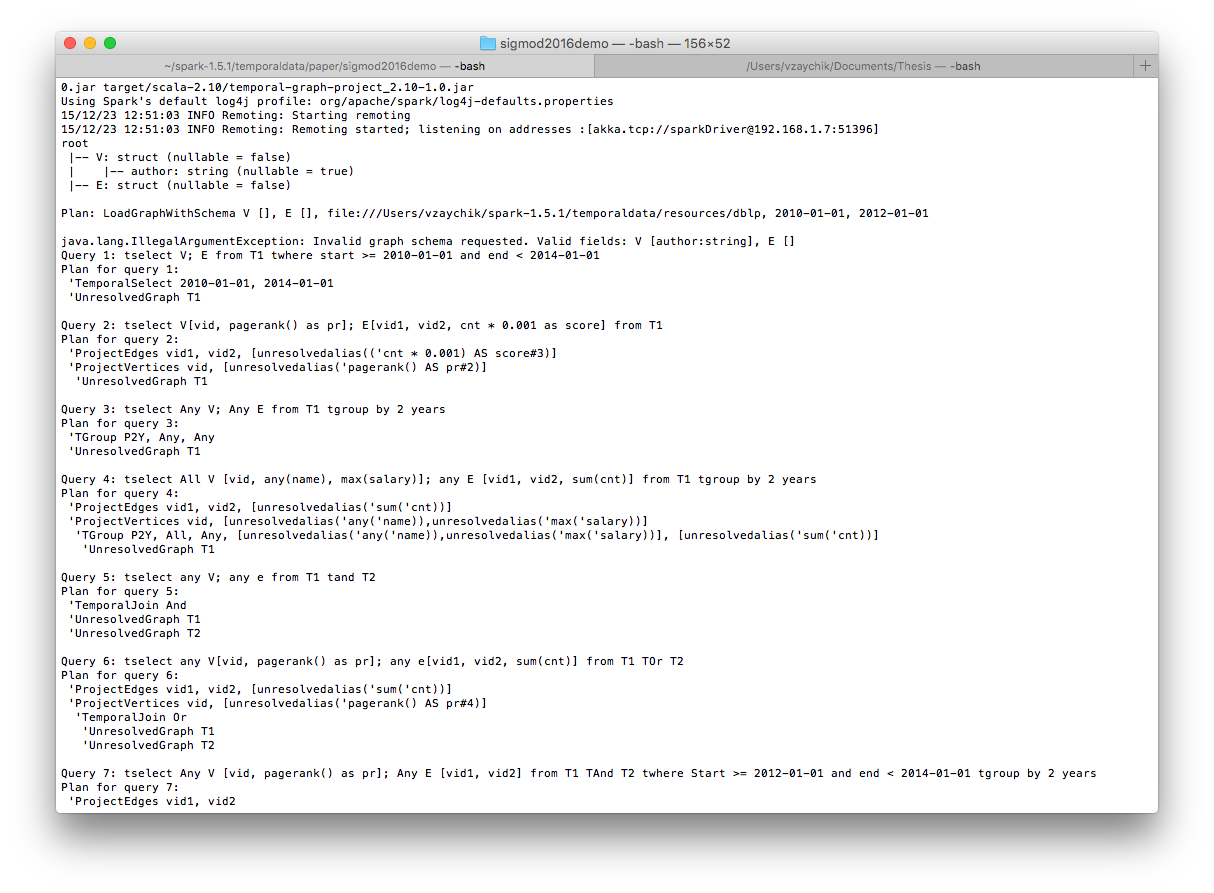
\includegraphics[width=3.4in]{figs/shell.png}
\vspace{-0.5cm}
\caption{\sys interactive shell.}
\vspace{-0.5cm}
\label{fig:shell}
\end{figure}

{\bf Interactive shell. Integration with SQL.}  \sys includes an
interactive shell for exploratory data analysis
(Figure~\ref{fig:shell}). Shell users can execute queries, define
(materialized) views, inspect query execution plans, and execute SQL
queries with an embedded \ql view. Consider the following SQL query
that returns \insql{vid} and \insql{tr} values of 20 vertices with the
most significantly increasing PageRank trend.

\begin{small}
\begin{verbatim}
Select VF.vid, VF.tr
From T5.vertices() as VF
Order by tr Limit 20
\end{verbatim}
\end{small}

An important part of the query is the use of \insql{T5.vertices()} in
the \insql{From} clause. This is an operation provided by the \sys
framework, which takes as input all vertices of \insql{T5} and their
attributes in a single nested relation \insql{VF}, with schema
\insql{(vid:long, start:date, end:date, tr:float)}. \insql{VF} can be
used in SQL queries. \sys also provides an operation \insql{edges()}
that returns a similar relation for the edges of a given \tg.




%\section{Experimental Evaluation}
\label{sec:exp}

\begin{figure*}[t]
\vspace{-0.2in}
\centering
\begin{minipage}[b]{2.1in}
\centering
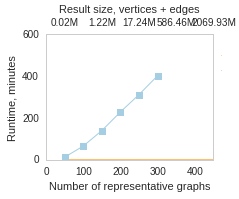
\includegraphics[width=2.1in]{figs/slice_ngrams_build13.png}
\vspace{-0.2in}
\caption{Slice on nGrams.}
\label{fig:slicengrams}
\vspace{-0.1in}
\end{minipage}
\begin{minipage}[b]{2.2in}
\centering
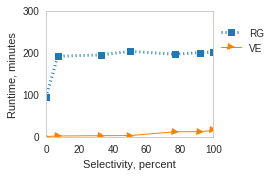
\includegraphics[width=2.4in]{figs/subgraph_ngrams_build13.png}
\vspace{-0.2in}
\caption{Subgraph on nGrams.}
\label{fig:subgraphngrams}
\vspace{-0.1in}
\end{minipage}
\begin{minipage}[b]{2.15in}
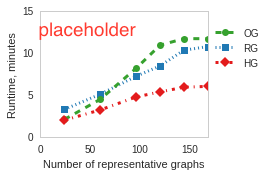
\includegraphics[width=2.15in]{figs/deg_twitter_build14.png}
\vspace{-0.2in}
\caption{Aggregate on Twitter.}
\label{fig:degtwitter}
\vspace{-0.1in}
\end{minipage}
\end{figure*}

\begin{figure*}[t!]
\centering
\begin{subfigure}{0.3\textwidth}
%\begin{minipage}{2.2in}
%\centering
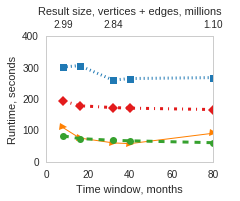
\includegraphics[width=2.2in]{figs/agg_allall_wikitalk_build13.png}
\caption{$q_v=\insql{always}$, $q_e=\insql{always}$, wiki-talk}
\label{fig:agg1}
%\end{minipage}
\end{subfigure}
\begin{subfigure}{0.3\textwidth}
%\begin{minipage}{2.2in}
%\centering
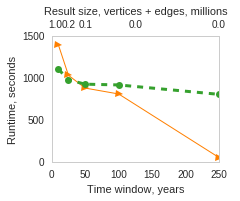
\includegraphics[width=2.2in]{figs/agg_allexists_ngrams_build13.png}
\caption{$q_v=\insql{always}$, $q_e=\insql{exists}$, nGrams}
\label{fig:agg2}
%\end{minipage}
\end{subfigure}
\begin{subfigure}{0.35\textwidth}
%\begin{minipage}{2.5in}
%\centering
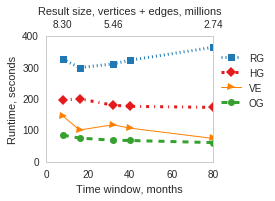
\includegraphics[width=2.3in]{figs/agg_allexists_wikitalk_build13.png}
\caption{$q_v=\insql{always}$, $q_e=\insql{exists}$, wiki-talk}
\label{fig:agg4}
%\end{minipage}
\end{subfigure}
\caption[]{Node creation with temporal windows.}
\vspace{-0.1in}
\label{fig:agg}
\end{figure*}

\subsection{Setup}
\label{sec:exp:setup}

All experiments were conducted on a 16-slave in-house Open Stack
cloud, using Linux Ubuntu 14.04 and Spark v2.0.  Each node has 4 cores
and 16 GB of RAM.  Spark Standalone cluster manager and Hadoop 2.6
were used.
%
Because Spark is a lazy evaluation system, a materialize operation was
appended to the end of each query, which consisted of the count of
nodes and edges.  Each experiment was conducted 3 times with a cold
start -- the running time includes the setup time of submitting the
job to the cluster manager, uploading the jar to the cluster, reading
the data from disk, building the chosen representation, and running
a single query.  We report the average running time, which is
representative because we took great care to control variability:
standard deviation for each measure is at or below 5\% of the mean
except in cases of very small running times.  No computation results
were shared between subsequent runs.

\eat{OG and HG inherit their implementation of \insql{slice}, \insql{map}
and \insql{subgraph} from RG and are not included in these
experiments.  Performance of all 4 data structures is compared in
\insql{aggregation}, \insql{union} and \insql{intersection}.}

{\bf Data.}  We evaluate performance of our framework on three real
open-source datasets, summarized in Table~\ref{tab:datasets}.
wiki-talk (\url{http://dx.doi.org/10.5281/zenodo.49561}) contains over
10 million messaging events among 3 million wiki-en users\eat{2002
  through 2015}, aggregated at 1-month resolution.\\nGrams
(\url{http://storage.googleapis.com/books/ngrams/books/datasetsv2.html})
contains word co-occurrence pairs\eat{ from 1520 through 2008}, with
30 million word nodes and over 2.5 billion undirected edges.  The
Twitter social graph~\cite{Gabielkov:2014:SSN:2591971.2591985}
contains over 23 billion directed follower relationships between 0.5
billion twitter users\eat{ collected in 2012}, sampled at 1-month
resolution.\eat{ based on account creation information from April
  2006.} \eat{DELIS contains monthly snapshots of a portion of the Web
  graph focusing on the .uk domains from 05/2006 through
  05/2007~\cite{BSVLTAG}. }The datasets differ in size, in the number
and type of attributes and in evolution rates, calculated as the
average graph edit similarity~\cite{Ren2011}. \eat{the evolutionary
  properties: co-authorship network nodes and edges have limited
  lifespan, while the nGrams network grows over time, with nodes and
  edges persisting for long duration.  All figures in the body of this
  section are on the larger nGrams dataset.  Refer to the Appendix for
  the DBLP figures, which show similar trends as nGrams.}

\eat{The behavior of the four physical representations reported below is
dependent on the underlying data format on disk
(Section~\ref{sec:sys:maint}), and should be interpreted in that
context.}

\subsection{Individual operators}
\label{sec:exp:ops}

{\bf Slice} performance was evaluated by varying the slice time window
and materializing the \tg, and is presented in
Figures~\ref{fig:slicengrams} for nGrams and~\ref{fig:slicewiki} for
wiki-talk (in Appendix~\ref{sec:app2}).  Similar trends were observed
for twitter.  Slice is expected to be more efficient when executed
over VE when data is coalesced on disk than over \sg, and we observe
this in our experiments.  This is because multiple passes over the
data are required for \sg to compute each representative graph,
leading to linear growth in running times for file formats and systems
without filter pushdown, as is the case here.  Slice over VE simply
executes temporal selection and has constant running times (29 sec for
wiki-talk, about 1.5 min for nGrams).\eat{Recall that in VE
  \insql{slice} performs temporal selection, and method when data on
  disk is coalesced.  \sg, in contrast, does multiple passes of select
  over the same data to compute each RG.  Thus, as expected, VE
  behavior is directly dependent on the size of input data regardless
  of the slice size for file formats and systems without filter
  pushdown, as is the case here, or if the data does not have temporal
  locality (Figure~\ref{fig:slicewiki}, Figure~\ref{fig:slicengrams}
  -- about 1.5 minutes for VE).  \sg behavior is linear in the slice
  size. } This experiment essentially measures the cost of
materializing \sg from its on-disk representation. \eat{ We observed the
same linear trend in our preliminary work, when the data was stored as
individual snapshots on disk, although less redundant work is needed
in that case.}

{\bf Vertex subgraph} performance was evaluated by specifying a
condition on the $length(a.attr)<t$ of the vertex attribute, with
different values of $t$ leading to different selectivity.  This
experiment was executed for wiki-talk (with $username$ as the
property) and for nGrams (with $word$ as the property).  Twitter has
no vertex attributes and was not used in this experiment.
Figure~\ref{fig:subgraphngrams} shows performance for \sg and VE on
nGrams (wiki-talk results in Appendix~\ref{sec:app2}).  Performance on
\sg is a function of the number of intervals and is insensitive to the
selectivity.  The behavior on VE is dominated by FK enforcement:
with high selectivity (few vertices) broadcast join affords
performance linear in the number of edges, whereas for a large number
of vertices broadcast join is infeasible and a hash-join is used
instead, which is substantially slower.  VE provides an order of
magnitude better performance than \sg: up to 3 min with hash-join and
up to 15 min with broadcast join for VE, in contrast to between 95 and
200 min for \sg.

{\bf Map}\eat{ We evaluate \insql{map} performance by varying the data
  size through the \insql{slice} operation.} exhibits a similar trend
as \insql{slice}: constant running time for VE and a linear increase
in running time with increasing number of representative graphs for
\sg (Figure~\ref{fig:project} for wiki-talk in
Appendix~\ref{sec:app2}, similar for other datasets).  Performance of
\insql{map} is slightly worse than that of \insql{slice} because
\insql{map} must coalesce its output as the last step, while
\insql{slice} does not.

\begin{table}
\caption{Experimental datasets.}
\vspace{-0.1in}
\small
\begin{tabular}{l | c | c | c | c }
\hline
\multicolumn{1}{l|}{\bfseries Dataset} & \multicolumn{1}{c|}{\bfseries |V|} & \multicolumn{1}{c|}{\bfseries |E|} & \multicolumn{1}{c|}{\bfseries Time Span} & \multicolumn{1}{c}{\bfseries Evol. Rate} \\ \hline
wiki-talk-en & 2.9M & 10.7M & 2002--2015 & 14.4 \\ \hline
nGrams & 29.3M & 2.5B & 1520--2008 & 16.67 \\ \hline
%%DELIS & 128M & 40.5B & 2006--2007 & ? \\ \hline
twitter & 505.4M & 23B & 2006--2012 & 88 \\ \hline
\end{tabular}
\vspace{-0.1cm}
\label{tab:datasets}
\end{table}

\begin{figure*}[t]
\begin{minipage}{2.1in}
\centering
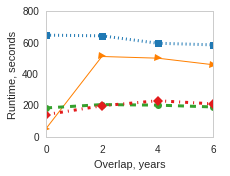
\includegraphics[width=2.1in]{figs/union_wikitalk_build13.png}
\vspace{-0.2in}
\caption{Union on wiki-talk.}
\label{fig:union1}
\vspace{-0.1in}
\end{minipage}
\begin{minipage}{2.2in}
\centering
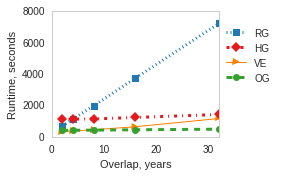
\includegraphics[width=2.5in]{figs/intersect_ngrams_build13.png}
\vspace{-0.2in}
\caption{Intersection on nGrams.}
\label{fig:intersectngrams}
\vspace{-0.1in}
\end{minipage}
\begin{minipage}{2.2in}
\centering
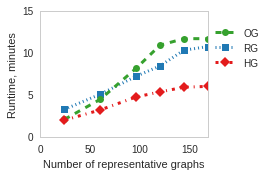
\includegraphics[width=2.4in]{figs/cc_wikitalk_build13.png}
\vspace{-0.2in}
\caption{Components on wiki-talk.}
\label{fig:ccwiki}
\vspace{-0.1in}
\end{minipage}
\end{figure*}

{\bf Aggregation} performance was evaluated on the graph-based
representations with a computation of vertex degrees, varying the size
of the temporal window obtained with slice.  The results in
Figure~\ref{fig:degtwitter} indicate that materialization of each
representative graph required for \sg makes it not a viable candidate
for this operation, especially over large datasets.  Both \og and \hg
exhibit linear increase in performance as the slice size is increased,
with a small slope.  Similar performance was observed in the other
datasets.

{\bf Node creation} performance was evaluated on all representations,
since all have different implementations of this operator.  We
executed topology-only creation (no attributes), varying the size
of the temporal window.  We observe that performance depends heavily
on the quantification, and on the data evolution rate.  \og is an
aggregated data structure with good temporal locality and thus in most
cases provides good performance and is insensitive to the temporal
window size (Figure~\ref{fig:agg1}).  However, in datasets with a
large number of representative graphs (such as nGrams), \og is slow on
large windows, an order of magnitude worse than VE in the worst case
(Figure~\ref{fig:agg2}).  VE outperforms \og when vertex and edge
quantification levels match (Figure~\ref{fig:agg1}), but is worse than
\og when vertex quantification is stricter than edge quantification
and FK must be enforced (Figure~\ref{fig:agg4}).  \og also outperforms
VE when both evolution rate is low and aggregation window is small
(Figure~\ref{fig:agg1}, wiki-talk).\eat{ \sg and \hg do not provide
  the best performance on any of our datasets.}

{\bf Union, intersection, and difference} by structure were evaluated
by loading two time slices of the same dataset with varying temporal
overlap.  Performance depends on the size of the overlap (in the
number of representative graphs) and on the evolution rate.  VE has
best performance when overlap is small (Figure~\ref{fig:union1})\eat{
  and when the evolution rate is high (Figure~\ref{fig:union2}),
  regardless of the size of the overlap}.  \og always has good
performance, constant w.r.t. overlap size.  This is expected, since
\og \insql{union} and \insql{intersection} are implemented as joins
(outer or inner) on the vertices and edges of the two operands.  VE,
on the other hand, splits the coalesced vertices/edges of each of the
two operands into intervals first, takes a union, and then reduces by
key.  When evolution rate is low and duration of an entity is high,
such as in wiki-talk for vertices, the split produces a lot of tuples
to then reduce, and performance suffers (Figure~\ref{fig:union1}). \sg
only has good performance on \insql{intersection} when few
representative graphs overlap, and never on \insql{union}
(Figure~\ref{fig:intersectngrams}). \hg performance is worse than \og,
by a constant amount in \insql{union}, and diverges in
\insql{intersection}.  \eat{\insql{difference} performance is similar
  to \insql{intersection}.}

{\bf Analytics.}  We implemented PageRank (PR) and Connected
Components (CC) analytics for the three graph-based representations
using the Pregel GraphX API.  PR was executed for 10 iterations or
until convergence, whichever came first. CC was executed until
convergence with no limit on the number of iterations.  Performance of
Pregel-based algorithms depends heavily on the partitioning strategy,
with best results achieved where cross-partition communication is
small~\cite{MoffittTempWeb16}.  For this reason, we evaluated only
with the E2D strategy.
%
Performance was evaluated on time slices of varying size.  Recollect
that analytics are essentially multiple rounds of aggregate
operations, so the performance we observe is an amplified version of
aggregate performance.  For a very small number of graphs (1-2), \sg
provides good performance, but slows down linearly as the number of
graphs increases.  \hg provides the best performance on analytics
under most conditions, with a linear increase but a significantly
slower rate of growth.  The tradeoff between \og and \hg depends on
graph evolution characteristics.  If the graph is a growth-only
evolution (such as in Twitter), \og is not denser than \hg and
computes everything in a single batch, which leads to the fastest
performance, as can be seen in Figure~\ref{fig:pranktwitter}.  If the
edge evolution represents more transient connections, then \hg is less
dense and scales better (Figure~\ref{fig:ccwiki}).  Note that \og and
\hg performance could be further improved by computing them over
coalesced structure-only V and E, and ignoring attributes.

{\bf In summary,} no one data structure is most efficient across all
operations.  This opens the door to query optimization based on the
characteristics of the data such as graph evolution rate and on the
type of operation being performed.  

\eat{VE provides the best
  performance for slice, map, and subgraph.  \og is efficient for
  aggregation under most conditions, and \hg for analytics.  The graph
  evolution rate is an important factor in selecting the more suitable
  representation.}

\subsection{Switching between representations}
\label{sec:exp:scale}

\begin{figure*}[t]
\centering
\begin{minipage}{2.2in}
\centering
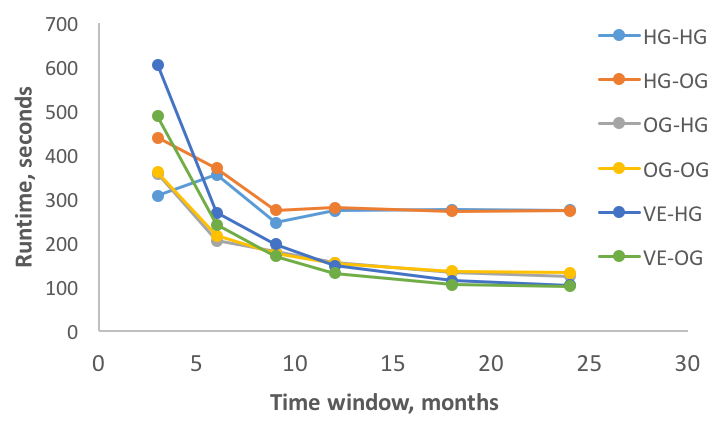
\includegraphics[width=2.1in]{figs/switch_cc.png}
%\vspace{-0.2in}
\caption{$\insql{node}^T_a$ followed by components.}
\label{fig:ncrtocc}
\vspace{-0.1in}
\end{minipage}
\begin{minipage}{2.2in}
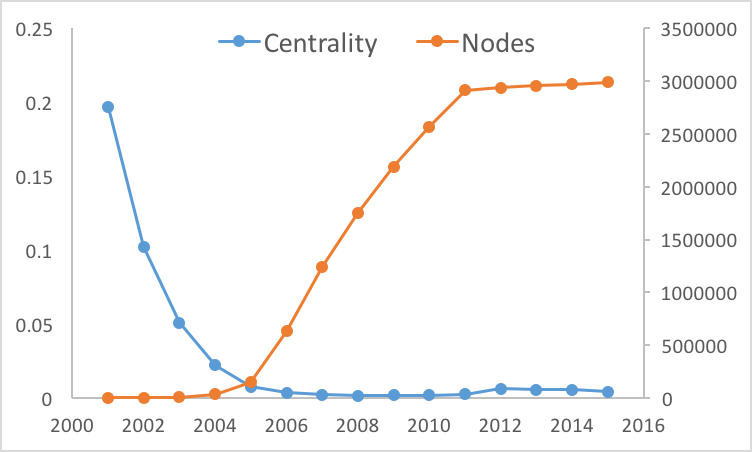
\includegraphics[width=2.2in]{figs/centrality.png}
\caption{In-degree centrality with 1 year resolution.}
\label{fig:central}
\end{minipage}
\begin{minipage}{2.2in}
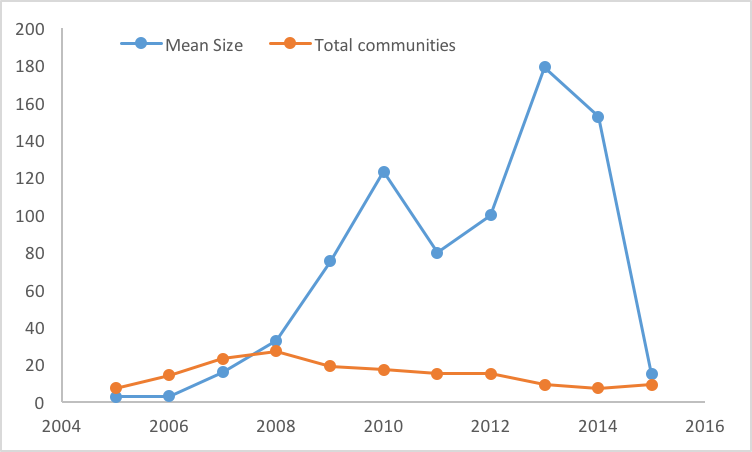
\includegraphics[width=2.2in]{figs/communities.png}
\caption{Communities with 1 year resolution.}
\label{fig:commun}
\end{minipage}
\end{figure*}

To treat the four representations as access methods, we need to be
able to switch between them.  The data structures can be created from
outputs of any of the four, at a cost.  To investigate the feasibility
of switching between representations, we executed two-operator queries
and either kept the representation constant or changed it between the
operators.  The query is based on the first two steps of example three
in our motivating use cases: node creation over temporal windows in
wiki-talk, followed by the connected components analytic.
Figure~\ref{fig:ncrtocc} shows the result of varying the size of the
temporal window.  Recall that \og is the best performing
representation for node creation at small windows and \hg for
components over this dataset.  The benefits of \hg are substantially
consumed by switching: the performance of \og-\og and and \og-\hg are
similar.  If the cost of switching was negligible, then \og-\hg should
have exhibited notably better performance than all other combinations.
However, the \og-\hg still performs best over-all, indicating that
switching is feasible.

\eat{{\bf Cluster Size.}  We next examine how the system performance scales
with the size of the cluster.  We execute
\insql{slice; aggregate(1 year, exists, exists); components}.}
%
\eat{
\begin{small}
\begin{verbatim}
   slice
   aggregate(1 year, exists, exists)
   connected components
   materialize vertices
\end{verbatim}
\end{small}
}
\eat{This query, executed on the wiki-talk dataset, computes connected
components over the past 10 years on the yearly scale.  Over the
twitter dataset the slice size is 2 years.}

%%\begin{small}
%%\begin{verbatim}
%%Q2. UKDELIS
%%
%%   aggregate(3 months, exists, always)
%%   pagerank(20 iterations)
%%   project pagerank score
%%   aggregate(12 months, exists, exists, trend)
%%   get top 10
%%\end{verbatim}
%%\end{small}
\eat{
This query, executed on DELIS dataset, computes stable links between
websites, i.e. links that persist for 3 months, and uses them to
compute pagerank for each.  The score is projected and its trend
computed in an aggregation over the whole dataset time period (1
year).  The top 10 websites with the highest increase in pagerank are
returned.
}

\eat{The best performing representation was selected based on our
experimental results.  Slice, project, and aggregate were performed
with VE, analytics with \hg.  The results are in
Table~\ref{tab:clustersize}.  Both queries show improvements in
running time as the cluster size grows, with diminishing returns.}
\eat{With the small wiki-talk dataset, performance improves initially
  with larger cluster sizes but levels off at the largest size.  With
  the large twitter dataset, ...}

\eat{
\begin{table}
\centering
\caption{Effect of cluster size, minutes.}
\vspace{-0.1in}
\small
\begin{tabular}{| l | c | c | c | c |}
\hline
\multicolumn{1}{|l|}{\bfseries Dataset} & \multicolumn{1}{c|}{\bfseries 4 slaves} & \multicolumn{1}{c|}{\bfseries 8 slaves} & \multicolumn{1}{c|}{\bfseries 12 slaves} & \multicolumn{1}{c|}{\bfseries 16 slaves}\\ \hline
wiki-talk & 8.41 & 6.02 & 5.02 & 2.94 \\ \hline
Twitter & 151.77 & 72.75 & 55.68 & 53.46 \\ \hline
\end{tabular}
\label{tab:clustersize}
\end{table}
}



\subsection{Use cases}
\label{sec:exp:cases}

To see how our algebra handles the use cases from
Section~\ref{sec:cases}, we implemented each one over the wiki-talk
dataset.  Each example requires a sequence of operators.  For each
operator we used the best performing data structures based on the
comparison experiments described above.

Example 1 answers the question of whether there are high influence
nodes and whether that behavior is persistent in time.  The code to
compute the answer is 4 lines of a Scala program and the query took 76
seconds to execute.  The results show that from 25 nodes with mean
degree of 40 and above that have persisted for at least 6 months, 6
have coefficient of variation below 50, which is quite low, and only 5
have it above 100.  This indicates that there are in fact high
in-degree nodes and that they continue to be influential over long
periods of time, despite the loose connectivity of the overall
network.

\eat{
\begin{verbatim}
    val deg = g.aggregateMessages[Int](triplet => { Iterator((triplet.dstId, 1)) }, (a, b) => {a+b}, 0, TripletFields.None).mapVertices((vid, intv, attr) => Map(intv -> attr._2), Map[Interval,Int]())
    val agg = deg.createNodes(ChangeSpec(g.getTemporalSequence.count.toInt), Exists(), Exists(), (a, b) => {a ++ b}, anyfun)()
    val unit = Resolution.from("P1M").unit
    println("lowest coefficient of variation (largest stability) top 10 users: " + agg.mapVertices((vid, intv, attr) => { val allpoints = TempGraphOps.makeSeries[Int](attr, Some(0)).map(x => x.getOrElse(0)); val mean = allpoints.sum / allpoints.size.toDouble; val variance = allpoints.map(x => math.pow(x - mean, 2)).reduce(_ + _) / allpoints.size; (mean, math.sqrt(variance) / mean * 100, allpoints.size)}, (0.0, 100.0, 1)).vertices.filter(x => x._2._2._1 > 0.0).sortBy(x => x._2._2._1, ascending = false).take(50).mkString("\n"))
\end{verbatim}
}

\eat{
\begin{figure}
\centering
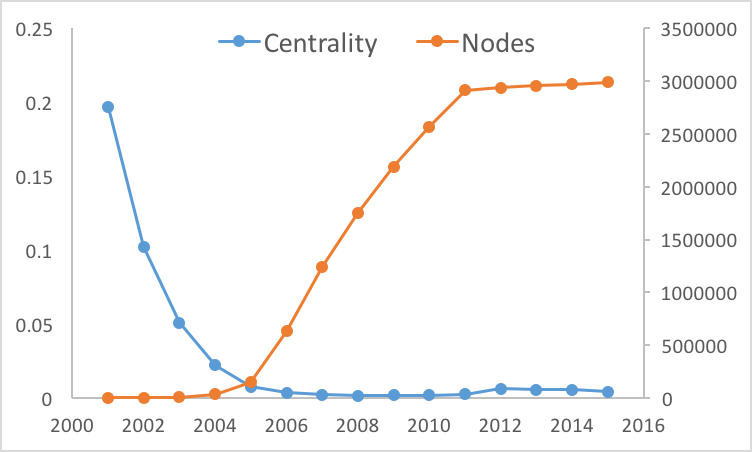
\includegraphics[width=2.2in]{figs/centrality.png}
\caption{In-degree centrality with 1 year resolution.}
\label{fig:central}
\end{figure}}

Example 2 examines how the graph centrality changes over time.  The
program is 6 lines of Scala code iterating with temporal windows of 1,
2, 3, 6, and 12 months, and the analysis took 25 minutes.  Results
show that regardless of the temporal resolution, the in-degree
centrality is extremely low, about 0.04.  Figure~\ref{fig:central}
provides an explanation -- as the size of the graph increases, its
centrality decreases.  Given that the number of edges in this graph is
only about 4 times the number of nodes, the graph is too sparse and
disjointed to have any centrality.

\eat{
\begin{table}
\centering
\caption{In-degree centrality over time in wiki-talk}
\small
\begin{tabular}{| l | c | c |}
\hline
\multicolumn{1}{|l}{\bfseries Window} & \multicolumn{1}{c|}{\bfseries Mean} & \multicolumn{1}{c|}{\bfseries StDev} \\ \hline
1 & 0.03 & 0.09 \\
2 & 0.04 & 0.11 \\
3 & 0.04 & 0.13 \\
6 & 0.06 & 0.18 \\
12 & 0.03 & 0.05 \\ \hline
\end{tabular}
\label{tab:centrality}
\end{table}
}

\eat{\begin{figure}
\centering
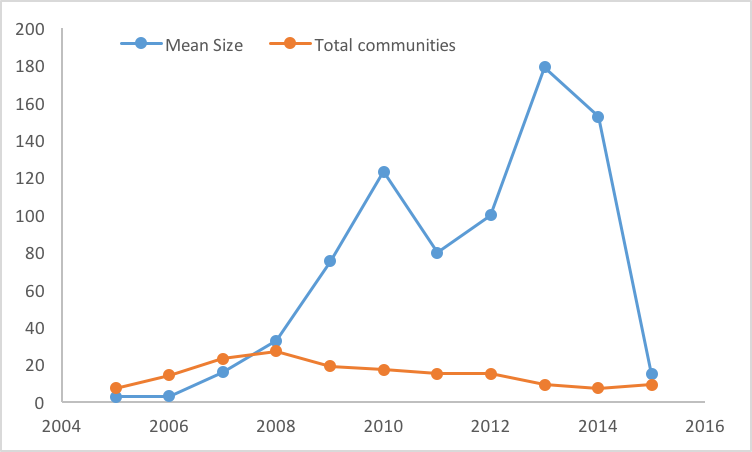
\includegraphics[width=2.2in]{figs/communities.png}
\caption{Communities with 1 year resolution.}
\label{fig:commun}
\end{figure}}

Finally, example 3 examines whether communities can be detected in the
wiki-talk network at different temporal resolution.  The program,
similar to the one above, is 6 lines of Scala code with varied
temporal windows.  The total runtime is 58 minutes.  Communities,
defined as connected components, can be detected in all temporal
resolutions.  As a reminder, the edge quantification in this query is
\insql{always}, so only edges that persist over each window are
retained.  The presence of communities even with large temporal
resolution indicates that communities form and persist over time.
Figure~\ref{fig:commun} shows the mean size of all communities by time
and their total number.  The peaks of the mean size, visible in all
temporal windows, may indicate that communities form and then reform
in a different configuration, perhaps for a different purpose.  The
results of this analysis can serve as a starting point to investigate
the large communities and what caused the size shifts.

{\bf In summary,} complex analyses can be expressed as queries in \ql
and lead to interesting insights about the evolution of the underlying
phenomena.\eat{  We leave the question of usability of the language for the
target audience to future work.}

\section{Conclusions and Future Work}
\label{sec:conc}

In this paper we presented \ql, a declarative query langauge for
evolving graphs.  We also proposed an implementation of \ql in scope
of Apache Spark, a distributed open-source processing framework.  We
implemented several physical representations of evolving graphs, and
several partitioning strategies, and studied their relative
performance for \ql operators.  

Our experiments demonstrate interesting trade-offs between spatial and
temporal locality.  This work opens many avenues for future work.  It
is in our immediate plans to start work on a query optimizer for \ql.
We will also implement and evaluate additional \tg representations
that explore the trade-off between density and compactness, and
between temporal and structural locality.  Finally, we are actively
working on extending the class of available trend analytics, and on
optimizing the performance of snapshot and trend analytics.

\eat{ While the Portal language is extensive, it is by no means
  complete. We recognize that there are a number of operations that
  are currently not supported but would be useful to potential users:}

\eat{\begin{enumerate}
\item Temporal pattern matching.  While aggregation provides an
  ability to detect some patters, a more general temporal-structural
  pattern mining is needed.  Work on specifying structural patterns in
  graphs is ongoing, however, at the time of this writing we are not
  aware of a general approach for specifying structural patterns that
  also have a time dimension.  For example, how should the user
  specify that he/she is looking for small strongly connected
  components that exhibit consistent growth over a period of time?
  Some work on this front has been done by Chan et
  al~\cite{Chan2008,Kan2009}.
\item Structural select (subgraph). 
\item Other kinds of temporal select besides by interval, such as with
  predicates, similar to snapshot selection support
  in~\cite{Khurana2013}. 
\item Across-time analytics (unlike spanshot-based analytics,
  e.g. pagerank) like the centrality metric for dynamic networks,
  where influence of a vertex propagates through time.
\item Anything that would return not another tgraph.  This could be
  measures of a whole graph (measure of centrality, degree
  distribution, diameter, etc.) or searching that returns a set of tgraphs,
  e.g. frequent pattern mining).
\end{enumerate}}


%\balance
\bibliographystyle{abbrv}
\bibliography{temporal}

\newpage
%\appendix \label{sec:app1}

Computing time periods during which no change occurred, necessary to
compute the \rgs view of a \tg.

\begin{small}
\begin{verbatim}
CREATE VIEW Changes(point) as (
  SELECT pstart FROM V  UNION  SELECT pend FROM V
  UNION
  SELECT pstart from E  UNION  SELECT pend FROM E
);

CREATE VIEW ChangesBefore(point, cnt) as (
  SELECT P1.point, count(*)
  FROM   Changes P1, Changes P2
  WHERE  P1.point >= P2.point
  GROUP BY P1.point
);

CREATE VIEW ChangePeriods(pstart, pend) as (
  SELECT P1.point as pstart, P2.point as pend
  FROM   ChangesBefore P1, ChangesBefore P2
  WHERE  P1.cnt+1 = P2.cnt
);
\end{verbatim}
\end{small}

\appendix \label{sec:app2}

Plots and discussion in this section complement experimental results
presented in Section~\ref{sec:exp}.

\begin{figure*}[t]
\centering
\begin{minipage}{3in}
  \centering
  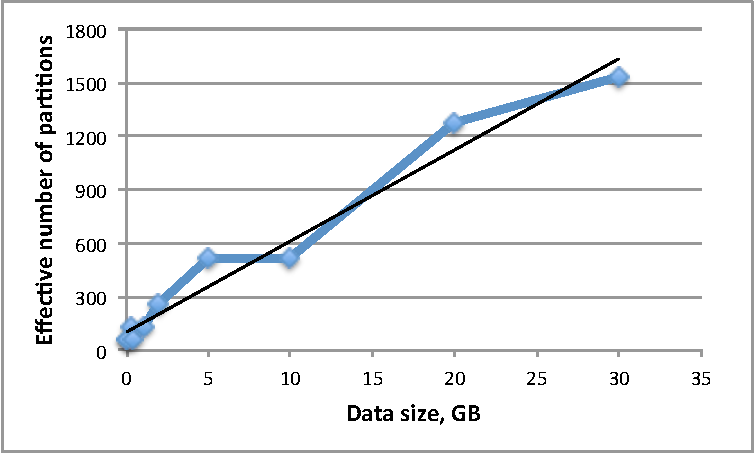
\includegraphics[width=2.7in]{figs/partsfit.pdf}
\vspace{-0.1in}
  \caption{Effective number of partitions.}
  \label{fig:partsfit}
\vspace{-0.1in}
\end{minipage}
\begin{minipage}{3in}
  \centering
  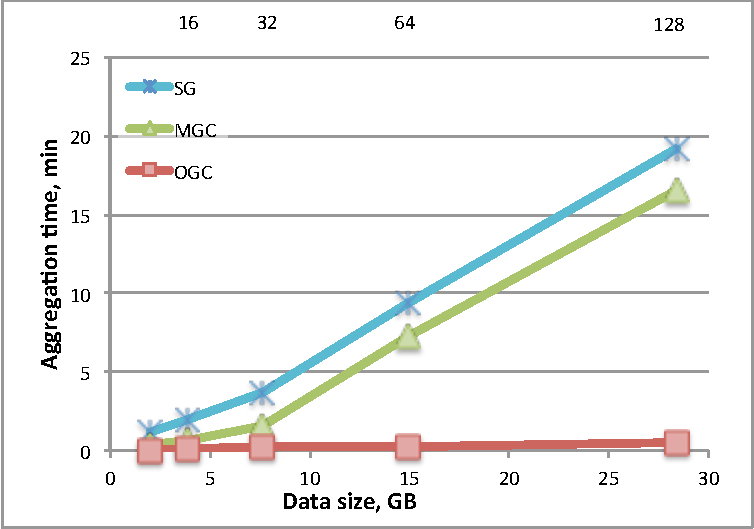
\includegraphics[width=2.7in]{figs/tgroupu_warm.pdf}
\vspace{-0.1in}
  \caption{\insql{TGroup} with \insql{All} (warm start).}
  \label{fig:tgroupu}
\vspace{-0.1in}
\end{minipage}
\end{figure*}

\begin{figure*}[t]
\centering
\begin{minipage}{3in}
  \centering
  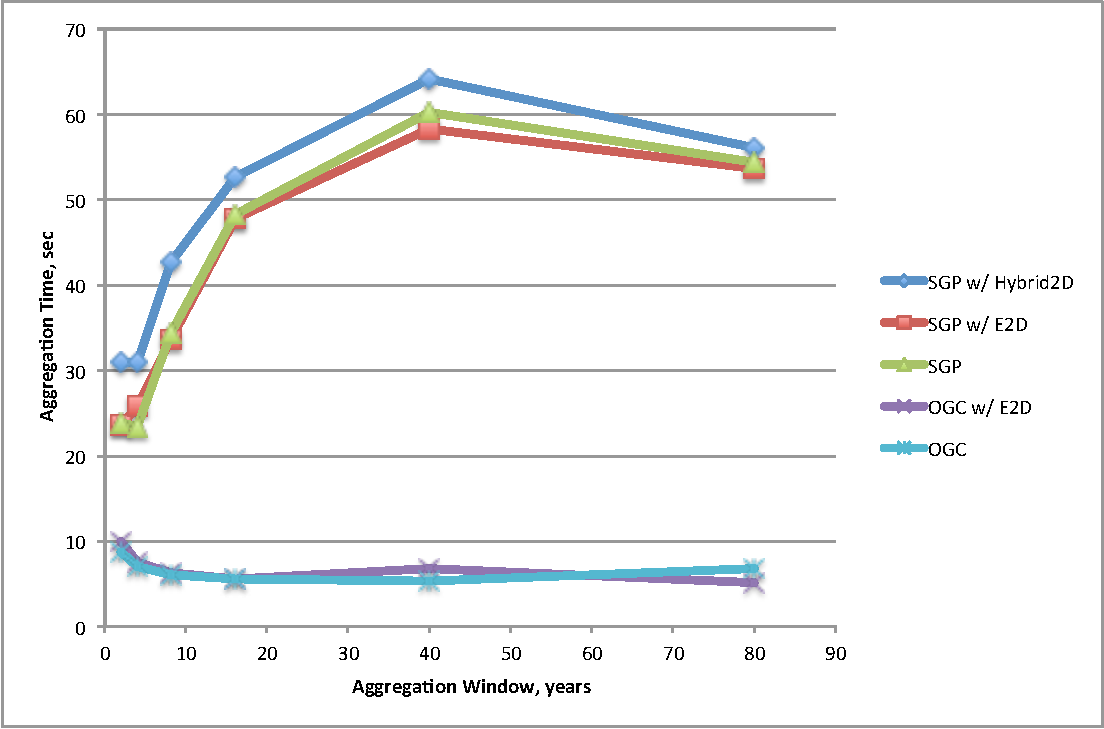
\includegraphics[width=2.7in]{figs/tgroupewidth.pdf}
\vspace{-0.1in}
  \caption{\insql{TGroup} by width, nGrams.}
  \label{fig:tgroup_width}
\vspace{-0.1in}
\end{minipage}
\begin{minipage}{3in}
  \centering
  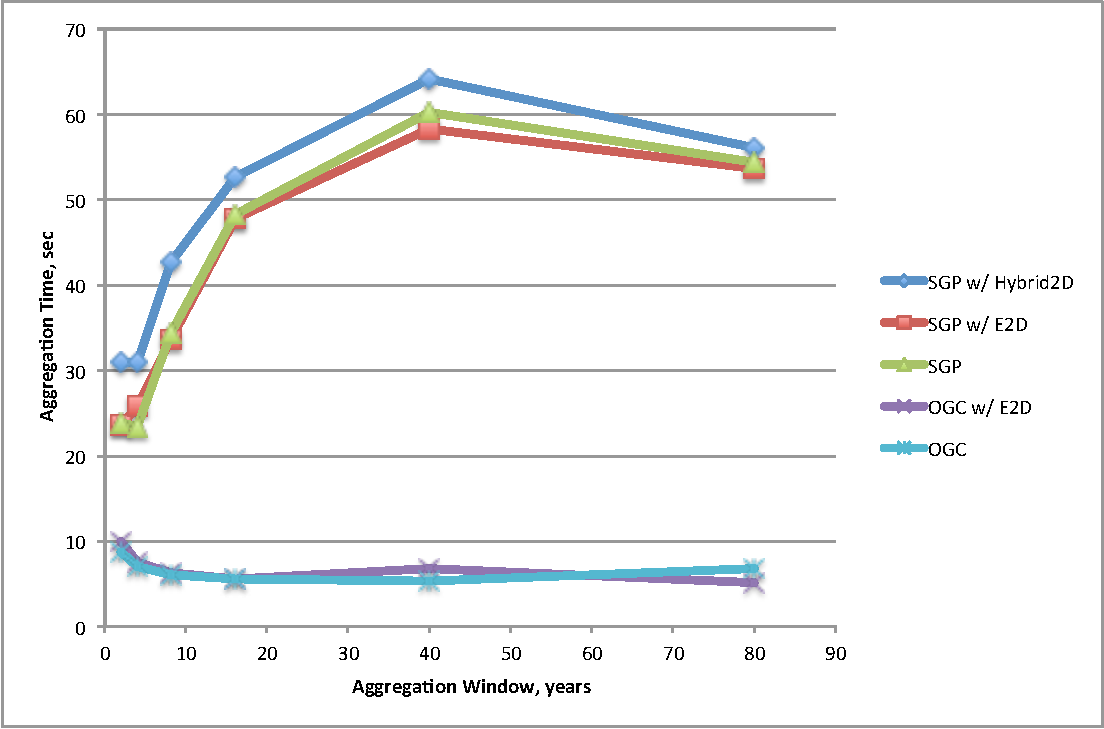
\includegraphics[width=2.7in]{figs/tgroupewidth_dblp.pdf}
\vspace{-0.1in}
  \caption{\insql{TGroup} by width, DBLP.}
  \label{fig:tgroup_width_dblp}
\vspace{-0.1in}
\end{minipage}
\end{figure*}

\begin{figure*}[t!]
\centering
\begin{minipage}{3in}
  \centering
  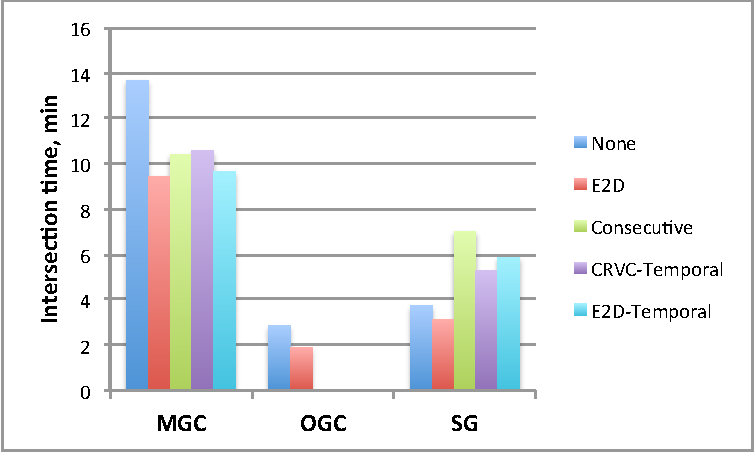
\includegraphics[width=2.7in]{figs/tand_parts.pdf}
\vspace{-0.1in}
  \caption{\insql{TAnd} by partition strategy, nGrams.}
  \label{fig:tand_parts}
\vspace{-0.1in}
\end{minipage}
\begin{minipage}{3in}
  \centering
  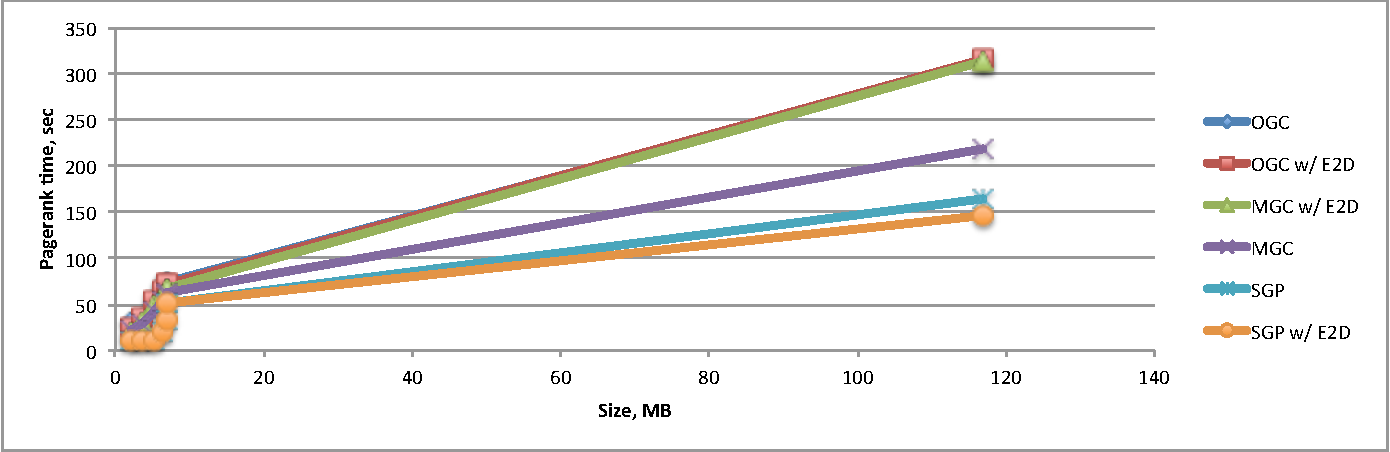
\includegraphics[width=2.7in]{figs/pagerank_dblp.pdf}
\vspace{-0.1in}
  \caption{PageRank time, DBLP.}
  \label{fig:pagerank_dblp}
\vspace{-0.1in}
\end{minipage}
\end{figure*}

Figure~\ref{fig:partsfit} complements Figure~\ref{fig:numparts}, in
which we presented the impact of number of partitions on the overall
performance.  In Figure~\ref{fig:partsfit} we show the linear trend
between the data size and the number of partitions that leads to
fastest execution.  The linear equation this fit produces is used in
the partition estimator during graph loading, except for very small
data sizes.

In Figure~\ref{fig:tgroupu} we show that \insql{TGroup} with
\insql{All} semantics exhibits the same behavior in all data
structures as \insql{TGroup} with \insql{Any} semantics in
Figure~\ref{fig:tgroupe}.  This is to be expected as both \insql{All}
and \insql{Any} use the same group by operation on the data, but with
different restrictions after grouping.

Another aspect of aggregation is the impact of an aggregation width.
Consider Figures~\ref{fig:tgroup_width} and
\ref{fig:tgroup_width_dblp} for the nGrams and the DBLP datasets,
respectively.  We fix the graph interval (128 and 80 snapshots,
respectively) and vary the width in powers of 2 up to total size.  For
each data structure we picked the most efficient partition strategy
based on the experiment in Section~\ref{sec:exp:tgroup},
Figure~\ref{fig:tgroupeparts}.  Observe that OGC and MGC are nearly
insensitive to the aggregation width, with small gains as the width
increases.  In contrast, SG performance logarithmically worsens as the
width increases in the DBLP dataset, but is largely unchanged for the
width values we evaluated in the nGrams dataset.

Figure~\ref{fig:tand_parts} complements Figure~\ref{fig:tandall}.  We
show that, similar to aggregation, partitioning improves performance
for temporal joins.  This finding is expected because co-partitioning
of two graphs along the same criteria improves the structural grouping
operation that is carried out. E2D partition strategy provides the
best performance, but the difference between it and the hybrid
strategies is not significant.

Finally, Figure~\ref{fig:pagerank_dblp} shows PageRank performance on
the DBLP dataset. Due to the very pronounced skew in the DBLP dataset,
the number of snapshots was drawn from the most recent to the left on
the timeline.  The same number of partitions was used for MGC/OGC
because the data size did not differ significantly between different
time intervals.  The general trend observed is the same as in the
nGrams dataset, with the only difference that at these small sizes the
E2D strategy does not produce an improvement in performance for MGC
and OGC.


\end{document}


